% Options for packages loaded elsewhere
\PassOptionsToPackage{unicode}{hyperref}
\PassOptionsToPackage{hyphens}{url}
%
\documentclass[
  a4paper,
]{scrbook}

\usepackage{amsmath,amssymb}
\usepackage{iftex}
\ifPDFTeX
  \usepackage[T1]{fontenc}
  \usepackage[utf8]{inputenc}
  \usepackage{textcomp} % provide euro and other symbols
\else % if luatex or xetex
  \usepackage{unicode-math}
  \defaultfontfeatures{Scale=MatchLowercase}
  \defaultfontfeatures[\rmfamily]{Ligatures=TeX,Scale=1}
\fi
\usepackage{lmodern}
\ifPDFTeX\else  
    % xetex/luatex font selection
  \setmainfont[]{Latin Modern Roman}
  \setsansfont[]{Latin Modern Roman}
\fi
% Use upquote if available, for straight quotes in verbatim environments
\IfFileExists{upquote.sty}{\usepackage{upquote}}{}
\IfFileExists{microtype.sty}{% use microtype if available
  \usepackage[]{microtype}
  \UseMicrotypeSet[protrusion]{basicmath} % disable protrusion for tt fonts
}{}
\makeatletter
\@ifundefined{KOMAClassName}{% if non-KOMA class
  \IfFileExists{parskip.sty}{%
    \usepackage{parskip}
  }{% else
    \setlength{\parindent}{0pt}
    \setlength{\parskip}{6pt plus 2pt minus 1pt}}
}{% if KOMA class
  \KOMAoptions{parskip=half}}
\makeatother
\usepackage{xcolor}
\setlength{\emergencystretch}{3em} % prevent overfull lines
\setcounter{secnumdepth}{5}
% Make \paragraph and \subparagraph free-standing
\ifx\paragraph\undefined\else
  \let\oldparagraph\paragraph
  \renewcommand{\paragraph}[1]{\oldparagraph{#1}\mbox{}}
\fi
\ifx\subparagraph\undefined\else
  \let\oldsubparagraph\subparagraph
  \renewcommand{\subparagraph}[1]{\oldsubparagraph{#1}\mbox{}}
\fi


\providecommand{\tightlist}{%
  \setlength{\itemsep}{0pt}\setlength{\parskip}{0pt}}\usepackage{longtable,booktabs,array}
\usepackage{calc} % for calculating minipage widths
% Correct order of tables after \paragraph or \subparagraph
\usepackage{etoolbox}
\makeatletter
\patchcmd\longtable{\par}{\if@noskipsec\mbox{}\fi\par}{}{}
\makeatother
% Allow footnotes in longtable head/foot
\IfFileExists{footnotehyper.sty}{\usepackage{footnotehyper}}{\usepackage{footnote}}
\makesavenoteenv{longtable}
\usepackage{graphicx}
\makeatletter
\def\maxwidth{\ifdim\Gin@nat@width>\linewidth\linewidth\else\Gin@nat@width\fi}
\def\maxheight{\ifdim\Gin@nat@height>\textheight\textheight\else\Gin@nat@height\fi}
\makeatother
% Scale images if necessary, so that they will not overflow the page
% margins by default, and it is still possible to overwrite the defaults
% using explicit options in \includegraphics[width, height, ...]{}
\setkeys{Gin}{width=\maxwidth,height=\maxheight,keepaspectratio}
% Set default figure placement to htbp
\makeatletter
\def\fps@figure{htbp}
\makeatother

\usepackage{booktabs}
\usepackage{longtable}
\usepackage{array}
\usepackage{multirow}
\usepackage{wrapfig}
\usepackage{float}
\usepackage{colortbl}
\usepackage{pdflscape}
\usepackage{tabu}
\usepackage{threeparttable}
\usepackage{threeparttablex}
\usepackage[normalem]{ulem}
\usepackage{makecell}
\usepackage{xcolor}
\usepackage{fancyhdr}
\usepackage{titling}
\setlength{\droptitle}{-2cm}
\preauthor{
  \begin{center}
  \Large
  \vspace{10mm}
  by
  \vspace{20mm}
}
\postauthor{
  \end{center}
  \vfill
}

\predate{
  \begin{center}
  A thesis 
  submitted in partial fulfilment of the \\
  requirements of the degree of \\
  Doctor of Philosophy in Physics\\               % Degree
  School of Physical and Chemical Sciences\\          % Department
  Te Herenga Waka - Victoria University of Wellington\\                       % University 
  \vspace{5mm}
}
\postdate{
  \\
  
\includegraphics[width=3in,height=1.5in]{figures/VUW-logo.png}\\
  \end{center}
  }

\renewcommand{\topfraction}{.8}
\renewcommand{\floatpagefraction}{.8}
\clubpenalty=9996
\widowpenalty=9999
\makeatletter
\makeatother
\makeatletter
\@ifpackageloaded{bookmark}{}{\usepackage{bookmark}}
\makeatother
\makeatletter
\@ifpackageloaded{caption}{}{\usepackage{caption}}
\AtBeginDocument{%
\ifdefined\contentsname
  \renewcommand*\contentsname{Table of contents}
\else
  \newcommand\contentsname{Table of contents}
\fi
\ifdefined\listfigurename
  \renewcommand*\listfigurename{List of Figures}
\else
  \newcommand\listfigurename{List of Figures}
\fi
\ifdefined\listtablename
  \renewcommand*\listtablename{List of Tables}
\else
  \newcommand\listtablename{List of Tables}
\fi
\ifdefined\figurename
  \renewcommand*\figurename{Figure}
\else
  \newcommand\figurename{Figure}
\fi
\ifdefined\tablename
  \renewcommand*\tablename{Table}
\else
  \newcommand\tablename{Table}
\fi
}
\@ifpackageloaded{float}{}{\usepackage{float}}
\floatstyle{ruled}
\@ifundefined{c@chapter}{\newfloat{codelisting}{h}{lop}}{\newfloat{codelisting}{h}{lop}[chapter]}
\floatname{codelisting}{Listing}
\newcommand*\listoflistings{\listof{codelisting}{List of Listings}}
\makeatother
\makeatletter
\@ifpackageloaded{caption}{}{\usepackage{caption}}
\@ifpackageloaded{subcaption}{}{\usepackage{subcaption}}
\makeatother
\makeatletter
\@ifpackageloaded{tcolorbox}{}{\usepackage[skins,breakable]{tcolorbox}}
\makeatother
\makeatletter
\@ifundefined{shadecolor}{\definecolor{shadecolor}{rgb}{.97, .97, .97}}
\makeatother
\makeatletter
\makeatother
\makeatletter
\makeatother
\ifLuaTeX
  \usepackage{selnolig}  % disable illegal ligatures
\fi
\usepackage[citestyle = ieee,urldate = iso8601]{biblatex}
\addbibresource{references.bib}
\IfFileExists{bookmark.sty}{\usepackage{bookmark}}{\usepackage{hyperref}}
\IfFileExists{xurl.sty}{\usepackage{xurl}}{} % add URL line breaks if available
\urlstyle{same} % disable monospaced font for URLs
\hypersetup{
  pdftitle={Developing an Insect Odorant Receptor Bioelectronic Nose for Vapour-Phase Detection},
  pdfauthor={Eddyn Oswald Perkins Treacher},
  hidelinks,
  pdfcreator={LaTeX via pandoc}}

\title{Developing an Insect Odorant Receptor Bioelectronic Nose for
Vapour-Phase Detection}
\author{Eddyn Oswald Perkins Treacher}
\date{Oct 2024}

\begin{document}
\frontmatter

\maketitle

\clearpage
\newpage
\thispagestyle{empty} % Hide header and footer on this page
\mbox{~}
\clearpage
\newpage

%----------------------------------------------
%   Abstract
%----------------------------------------------

\thispagestyle{plain}

\begin{flushleft}
% Manually add a section to the table of contents
\pagenumbering{roman}
\addcontentsline{toc}{chapter}{Abstract}
\huge\textbf{Abstract}
\end{flushleft}

\vspace*{\baselineskip}

The ability to detect volatile organic compounds in a highly sensitive and selective manner is desirable for applications as varied as diagnosis of illnesses at a remote clinic, monitoring of air in an industrial setting, or identification of invasive organisms at a biosecurity checkpoint. Historically, animal noses have been used for such tasks, as their combined sensitivity and selectivity are greatly superior to traditional artificial sensors. However, training and deploying animals in such situations is both time and cost intensive. In recent years, an improved understanding of \textit{in vivo} biological sensing has led to efforts to mimic these highly efficient processes in an artificial sensor format. \\[5pt] To this end, a “bioelectronic nose” was developed. This sensor uses an artificial transducer to amplify responses of an insect olfactory system to specific volatile compounds. Thin-film transistors were used as the amplifier element, given their low cost, small size and extreme sensitivity. Various thin-film morphologies were compared, and their suitability for bioelectronic nose development assessed. Transducers made using a novel steam-assisted thin-film deposition technique were found to have highly consistent device-to-device electrical properties relative to other films. Films made using this process typically showed more surface contamination than other morphologies, but their high sensitivity was nonetheless confirmed with a non-specific sensing series in an aqueous environment. \\[5pt] One of the major challenges encountered in this thesis was variability in the quality of sensor functionalisation. Raman spectroscopy and fluorescence microscopy confirmed an existing non-covalent attachment method could successfully immobilise nanodiscs onto the transistor channel region. However, various sensors functionalised using the same procedure often exhibited no sensing activity. Extensive electrical characterisation indicated the presence of an unidentified contamination layer preventing electrical interaction between the insect odorant receptors and transducer thin-film. It was shown that this layer was unlikely to be directly associated with the thin-film morphology used for the transducer. \\[5pt] Subsequently, an alternative biotin-based non-covalent method which eliminated several possible contamination sources was trialled. This alternative biotin-based method was used to demonstrate successful aqueous sensing of femtomolar concentrations of methyl salicylate by an iOR10a-functionalised device. When tested in a custom-built vapour delivery system, a similar bioelectronic sensor was shown to be highly sensitive to the target vapour. However, consistent reproduction of the biotin-based method was challenging due to the invasive cleaning method involved. It was therefore difficult to determine conclusively whether sensor responses were selective. By finding new, systematic approaches to address the major barriers to sensor success carefully identified in this work, there are promising signs that a highly reliable vapour-phase bioelectronic nose can be produced.

%\fancyhf{} %clear all headers and footers fields
%\thispagestyle{fancy} % Change header and footer on this page
%\renewcommand{\headrulewidth}{0pt}
%\fancyhead[L]{\textit{Abstract}} % Set header content
%\fancyfoot[L]{\thepage} %prints the page number on the right side of the header

\clearpage
\newpage
\thispagestyle{empty} % Hide header and footer on this page
\mbox{~}
\clearpage
\newpage


%----------------------------------------------
%   Acknowledgement
%----------------------------------------------

\thispagestyle{plain}

\begin{flushleft}
% Manually add a section to the table of contents
\addcontentsline{toc}{chapter}{Acknowledgements}
\huge\textbf{Acknowledgements}
\end{flushleft}

\vspace*{\baselineskip}

I would first like to acknowledge the lands of my ancestors, and the lands of the sovereign first peoples to which my ancestors travelled. We each come from the land, live off the land and return to the land.\\[5pt]
\textit{Noon of Essex to Warrang, on the Friends, Autumn 1811} \\[5pt]
\textit{Cave of Cambridgeshire to Warrang, on the Royal Charlotte, Autumn 1825} \\[5pt]
\textit{Boyce of Suffolk to Warrang, 1832} \\[5pt] 
\textit{Charlton of Northumberland to Warrang, on the Clyde, Spring 1834} \\[5pt]
\textit{Prouse of Devonshire to Pito-one, on the Duke of Roxburgh, Summer 1840} \\[5pt]
\textit{Ebden of Devonshire to Pito-one, on the Tyne, Winter 1841} \\[5pt]
\textit{Collis of Hampshire to Pito-one, on the Birman, Autumn 1842} \\[5pt]
\textit{Swann of Loch Garman to Te Whanganui-a-Tara, 1844} \\[5pt] 
\textit{Blythe of Berkshire to Whakatū, circa 1846} \\[5pt]
\textit{Innes of Berkshire to Naarm, on the Sacramento, Autumn 1853} \\[5pt]
\textit{Sheppard of Gloucestershire to Naarm, 1853} \\[5pt] 
\textit{Bruce of London to Naarm, on the Omega, Autumn 1855} \\[5pt]
\textit{Quennell of Surrey to Warrang, on the Asiatic, Winter 1855} \\[5pt]
\textit{Barr of Glasgow to Kōpūtai, on the Sir Edward Paget, Winter 1856} \\[5pt] 
\textit{Perkins of London to Te Whanganui-a-Tara, on the Matoaka, Spring 1859} \\[5pt]
\textit{McKee of Antrim to Tāmaki Makaurau, on the Indian Empire, Spring 1862} \\[5pt]
\textit{Sandilands of Peeblesshire to Ōtepoti, circa 1864} \\[5pt] 
\textit{Treacher of Berkshire to Te Whanganui-a-Tara, on the Wild Duck, Summer 1865} \\[5pt]
\textit{McTaggart of Argyllshire to Kōpūtai, on the Edward P. Bouverie, Autumn 1869} \\[5pt] 
\textit{Chapman of Kent to Whakatū, on the Adamant, Winter 1874} \\[5pt]
\textit{Cheel of London to Whakatū, on the Queen Bee, Winter 1877} \\[5pt]  
\textit{Hutchison of Aberdeen to Tarntanya, before 1882.} \\[5pt] 
I chose to start my doctoral studies just a few months into a global pandemic. Completing a challenging project with a worldwide crisis in the background might have been impossible without the supervision of AProf. Natalie Plank. Her ability to adapt to and overcome any problem has taught me that there is no situation which is truly unmanageable. I am deeply grateful for her leadership throughout a time of particular chaos. \newpage
\fancyhf{} %clear all headers and footers fields
\thispagestyle{fancy} % Change header and footer on this page
\renewcommand{\headrulewidth}{0pt}
\fancyhead[L]{\textit{Acknowledgements}} % Set header content
\fancyfoot[L]{\thepage} %prints the page number on the left side of the header 
I started this project with minimal formal training in biological science, coming from a primarily physics and engineering background. \\[5pt] The immense support I received from Melissa Jordan and Colm Carraher from the Institute for Plant and Food Research (PFR) to complete this project meant that this was not an issue, and I thank them both immensely for this. \\[5pt] I would not have been able to begin this thesis without the financial backing and support I received from PFR and the Better Border Biosecurity (B3) programme. In particular, I am very grateful to Andrew Kralicek, formerly with PFR and now at Scentian Bio, and the ex-Director of B3, David Teulon, for helping to secure funding for my project. I would also like to thank the donor of the Ernest Marsden Scholarship in Physics for their significant financial support. \\[5pt] There are many incredibly supportive people who I worked alongside during my project. I would like to start off by thanking Rifat Ullah, whose mentoring and kindness encouraged me to pursue further study. His work on the initial design and setup of the vapour delivery system was invaluable to me throughout this project. I am also especially grateful to Alex Puglisi, for constructing the mechanical elements of the vapour delivery system and giving me extensive feedback on the system design. I would like to thank Peter Coard, for his advice and guidance when constructing the electrical elements of the vapour delivery system. I would also like to thank Selvan Murugathas for his advice on constructing the insect odorant receptor sensors, as well as Damon Colbert and Valentina Lucarelli, who provided the insect odorant receptor nanodiscs used in this work. \\[5pt] Thank you to AProf. Ben Ruck, my supportive secondary supervisor, and to AProf. Franck Natali, for always asking about my thesis in the tearoom. Thank you to Gideon Gouws for his friendly encouragement and advice. For their substantial technical assistance and mentoring during this project, I would also like to thank Alan Rennie, Grant Franklin, Chris Lepper, Rashika Gunasekara, Pete Jebson and Sushila Pillai from VUW, Andrew Chan from PFR, AProf. Charles Unsworth from the University of Auckland, and Prof. Simon Brown and his nanomaterials group from the University of Canterbury. \\[5pt] I was lucky enough to start my doctoral program just as a group of supportive and talented senior students were finishing, and finished just as a group of enthusiastic and talented new doctoral students were starting. A special thanks to Jenna Nyugen, Erica Happe and Erica Cassie for teaching me the fabrication processes and characterisation procedures that made this thesis happen; and a special thanks to Marissa Dierkes, Danica Fontein, Sangar Begzaad and Alireza Zare, for their incredible support throughout the thesis writing process. \\[5pt] I would further like to thank everyone else I shared an office with and worked alongside, including Jackson, Will, Roshni, Ali, Kira, Catherine, Martin, Janani, Ted, Kiri and Joe. I would also like to thank all the interns and summer students who I worked with during this project. \\[5pt] A massive thank you to Openstar Technologies. It has been an honour to work on a cutting-edge plasma physics project right here in Wellington. A particularly big thank you to Ratu, Darren, Thomas, Ben and Gabriel for having me as part of the team. Thank you also to the other Openstar interns, in particular the other physics interns, Valentina and Benjy. I sincerely hope to see fusion with net energy gain in Aotearoa New Zealand within the next decade. \\[5pt] I want to thank Shodokan Aikido New Zealand for their support throughout this thesis, in particular for the once-in-a-lifetime opportunity to travel to Osaka to be graded for first-dan by Nariyama Shihan. Thanks for all the training and support, Ian. Thank you to all the friends and family, old and new, who have supported me over these wild past few years. You know who you are. \\[5pt] Thank you to my brother, Keeson, and to my parents, Hilary and Phillip. Your support means everything to me, and I would not be where I am today without you. Our Friday lunchtime cafe visits inspired and motivated me throughout the doctoral program. Thank you, thank you, thank you for your love, your compassion, and for being there for me. \\[5pt] Finally, thank you Nina. Your love has kept me going through the most difficult and most wonderful times over the last three and a half years. You are the light of my life, and I am so happy to have taken on this challenge with you by my side. \\[5pt] Arohanui and peace to you all, Eddyn (Ned)

\fancyhf{} %clear all headers and footers fields
\thispagestyle{fancy} % Change header and footer on this page
\renewcommand{\headrulewidth}{0pt}
\fancyhead[R]{\textit{Acknowledgements}} % Set header content
\fancyfoot[R]{\thepage} %prints the page number on the right side of the header

\clearpage
\newpage
\thispagestyle{empty} % Hide header and footer on this page
\mbox{~}
\clearpage
\newpage

\pagestyle{headings}

\ifdefined\Shaded\renewenvironment{Shaded}{\begin{tcolorbox}[enhanced, boxrule=0pt, borderline west={3pt}{0pt}{shadecolor}, interior hidden, frame hidden, sharp corners, breakable]}{\end{tcolorbox}}\fi

\renewcommand*\contentsname{Table of Contents}
{
\setcounter{tocdepth}{2}
\addcontentsline{toc}{chapter}{Table of Contents}
\tableofcontents
}
\listoffigures
\addcontentsline{toc}{chapter}{List of Figures}
\listoftables
\addcontentsline{toc}{chapter}{List of Tables}

\clearpage
\newpage
\thispagestyle{empty} % Hide header and footer on this page
\mbox{~}
\clearpage
\newpage

%----------------------------------------------
%   List of Abbreviations
%----------------------------------------------

\thispagestyle{plain}

\begin{flushleft}
% Manually add a section to the table of contents
\addcontentsline{toc}{chapter}{List of Abbreviations}
\huge\textbf{List of Abbreviations}
\end{flushleft}

\vspace*{\baselineskip}

\begin{table}[H]
  \begin{tabular}{@{}p{0.25\textwidth} p{0.75\textwidth}@{}}  % Adjust the width as needed
    2D  & 2-Dimensional  \\[5pt]
    Ab  & Antibody  \\[5pt]
    AB  & Amyl Butyrate  \\[5pt]
    AB-NTA  & N$\alpha$,N$\alpha$-Bis(carboxymethyl)-\textit{L}-lysine hydrate  \\[5pt]
    AFM  & Atomic Force Microscope/Microscopy  \\[5pt]
    AH  & Absolute Humidity  \\[5pt]
    Avi-tag  & Avidin-tag  \\[5pt]
    BMIM  & 1-butyl-3-methylimidazolium bis(trifluoromethylsulfonyl)imide  \\[5pt]
    CAD  & Computer Aided Design \\[5pt]
    CNT  & Carbon Nanotube  \\[5pt]
    CVD  & Chemical Vapour Deposition  \\[5pt]
    Cy3  & Cyanine 3  \\[5pt]
    DAN  & 1,5-diaminonaphthalene  \\[5pt]
    DAQ  & Data Acquisition Input/Output Module  \\[5pt]
    DCB  & 1,2-dichlorobenzene  \\[5pt]
    DI  & Deionised  \\[5pt]
    DMF  & Dimethylformamide   \\[5pt]
    DMSO  & Dimethylsulfoxide   \\[5pt]
    DMT-MM   & 4-(4,6-dimethoxy-1,3,5-triazin-2-yl)-4 methylmorpholinium chloride \\[5pt]
    DMMP  & Dimethyl Methylphosphonate  \\[5pt]
    DNA  & Deoxyribonucleic Acid  \\[5pt]
    E2Hex  & \textit{trans}-2-hexan-1-al  \\[5pt]
    EB  & Ethyl Butyrate  \\[5pt]
    EDC  & 1-Ethyl-3-(3-dimethylaminopropyl)carbodiimide  \\[5pt]
    EDL  & Electric Double Layer  \\[5pt]
    EIS  & Electrochemical Impedance Spectroscopy  \\[5pt]
    EtHex  & Ethyl Hexanoate  \\[5pt]
    EtOH  & Ethanol  \\[5pt]
    FET  & Field-Effect Transistor  \\[5pt]
  \end{tabular}
\end{table}

\newpage
\fancyhf{} %clear all headers and footers fields
\thispagestyle{fancy} % Change header and footer on this page
\renewcommand{\headrulewidth}{0pt}
\fancyhead[L]{\textit{List of Abbreviations}} % Set header content
\fancyfoot[L]{\thepage} %prints the page number on the right side of the header
\begin{table}[H]
  \begin{tabular}{@{}p{0.25\textwidth} p{0.75\textwidth}@{}}  % Adjust the width as needed
    FITC  & Fluorescein isothiocyanate  \\[5pt]
    GA  & Glutaraldehyde  \\[5pt]
    GFET  & Graphene Field-Effect Transistor  \\[5pt]
    GFP  & Green Fluorescent Protein  \\[5pt]
    GPCR  & G-protein Coupled Receptor  \\[5pt]
    HEK  & Human Embryonic Kidney  \\[5pt]
    His-tag  & Histidine-tag  \\[5pt]
    hOR  & Human Odorant Receptor  \\[5pt]
    HPLC  & High-performance Liquid Chromatography   \\[5pt]
    iOR  & Insect Odorant Receptor  \\[5pt]
    IPA  & Isopropanol  \\[5pt]
    LOD  & Limit of Detection  \\[5pt]
    m-CNT  & Metallic Carbon Nanotube   \\[5pt]
    MeOH  & Methanol   \\[5pt]
    MeSal  & Methyl Salicylate   \\[5pt]
    MFC  & Mass Flow Controller   \\[5pt]
    mOR  & Mouse Odorant Receptor  \\[5pt]
    MOSFET  & Metal-Oxide-Semiconductor Field-Effect Transistor  \\[5pt]
    MSP  & Membrane Scaffold Protein  \\[5pt]
    MWCNT  & Multi-Walled Carbon Nanotube  \\[5pt]
    ND  & Nanodisc  \\[5pt]
    NHS  & N-Hydroxysuccinimide  \\[5pt]
    NMR  & Nuclear Magnetic Resonance  \\[5pt]
    NSB  & Non-Specific Binding   \\[5pt]
    NTA  & Nitrilotriacetic Acid   \\[5pt]
    OBP  & Odorant Binding Protein  \\[5pt]
    OR  & Odorant Receptor  \\[5pt]
    ORCO  & Odorant Receptor Co-Receptor  \\[5pt]
    PBA  & 1-Pyrenebutyric Acid  \\[5pt]
    PBASE  & 1-Pyrenebutanoic Acid N-hydroxysuccinimide Ester  \\[5pt]
    PBS  & Phosphate-Buffered Saline  \\[5pt]
    PCB  & Printed Circuit Board   \\[5pt]
  \end{tabular}
\end{table}

\newpage
\fancyhf{} %clear all headers and footers fields
\thispagestyle{fancy} % Change header and footer on this page
\renewcommand{\headrulewidth}{0pt}
\fancyhead[R]{\textit{List of Abbreviations}} % Set header content
\fancyfoot[R]{\thepage} %prints the page number on the right side of the header
\begin{table}[H]
  \begin{tabular}{@{}p{0.25\textwidth} p{0.75\textwidth}@{}}  % Adjust the width as needed
    PDL & Poly-\textit{D}-lysine  \\[5pt]
    PDMS  & Polydimethylsiloxane   \\  [5pt]
    PEG  & Polyethylene Glycol  \\[5pt] 
    PID  & Photoionisation Detector  \\[5pt] 
    PLL  & Poly-\textit{L}-lysine  \\[5pt]
    PPB  & Pyrene-PEG-Biotin  \\[5pt]
    PPF  & Pyrene-PEG-FITC  \\[5pt]
    PPN  & Pyrene-PEG-NTA  \\[5pt]
    PPR  & Pyrene-PEG-Rhodamine  \\[5pt]
    PTFE  & Polytetrafluoroethylene (Teflon™)  \\[5pt]
    PVC  & Polyvinyl chloride  \\[5pt]
    QCM  & Quartz Crystal Microbalance  \\[5pt]
    RH  & Relative Humidity  \\[5pt]
    RHI  & Relative Humidity and Temperature Indicator  \\[5pt] 
    RNA  & Ribonucleic Acid   \\[5pt]
    SAW  & Surface Acoustic Wave   \\[5pt]
    s-CNT  & Semiconducting Carbon Nanotube   \\[5pt]
    SEM  & Scanning Electron Microscope/Microscopy   \\[5pt]
    SMU  & Source Measure Unit   \\[5pt]
    SPR  & Surface Plasmon Resonance   \\[5pt]
    Sulfo-NHS  & N-hydroxysulfosuccinimide   \\[5pt]
    SWCNT  & Single-Walled Carbon Nanotube   \\[5pt]
    TFTFET  & Thin-Film Field-Effect Transistor  \\[5pt]
    TMAH  & Tetramethylammonium hydroxide  \\[5pt]
    TX  & Transfer Characteristics  \\[5pt]
    UV  & Ultraviolet  \\[5pt]
    VI  & Virtual Instrument  \\[5pt]
    VUAA1  & N-(4-Ethylphenyl)-2-{[4-ethyl-5-(pyridin-3-yl)-4H-1,2,4-triazol-3-yl]sulfanyl}acetamide  \\[5pt] 
  \end{tabular}
\end{table}

\clearpage
\newpage
\thispagestyle{empty} % Hide header and footer on this page
\mbox{~}
\clearpage
\newpage

% Adjust the top and bottom margins of float pages to center floats
\makeatletter
\setlength{\@fptop}{0pt plus 1fil}
\setlength{\@fpbot}{0pt plus 1fil}
\makeatother

\pagestyle{headings}
\mainmatter
\bookmarksetup{startatroot}

\hypertarget{introduction}{%
\chapter{Introduction}\label{introduction}}

\hypertarget{background}{%
\section{Background}\label{background}}

The `bioelectronic nose', an electronic transducer modified with
elements of the animal olfactory system, has the potential to allow
specific detection of airborne volatile compounds at concentrations as
low as parts per trillion
\autocite{Glatz2011,Kwon2015,Dung2018,Kim2022a}. An ideal transducer
platform is the thin-film transistor (TFT) which is particularly
portable, simple to use, small and robust
\autocite{Kauffman2008,Khan2020}. The thin films used in these
field-effect transistors (FETs) include carbon nanotube networks and
graphene, low-dimensional nanomaterials which are both highly sensitive
and biocompatible \autocite{Shkodra2021}. The implications of successful
development of such a portable and robust bioelectronic nose are
significant. Applications could be found in high-importance fields such
as biosecurity, medicine, environmental protection and food safety
\autocite{Dung2018,Arakawa2019,Yang2017,Son2017}. For example, it has
been demonstrated that it is possible to detect invasive brown
marmorated stinkbugs based on their volatile trace \autocite{Moser2020}.
A bioelectronic nose could potentially accomplish this biosecurity task
far more cheaply and efficiently than trained sniffer dogs
\autocite{Lee2010,Moon2020,Terutsuki2020}. There has been rapid progress
in the development of bioelectronic noses using carbon nanotube
field-effect transistors (CNT FETs) and graphene field-effect
transistors (GFETs) over the past 15-20 years
\autocite{Yoon2009,Lee2010,Yang2018}.

Insect odorant receptors (iORs) enable simple invertebrates, such as the
vinegar fruit fly \emph{Drosophila melanogaster}, to distinguish between
a huge number of specific volatile compounds
\autocite{Hallem2004,Smart2008,Wicher2008,Munch2016,Bohbot2020}. Within
the past five years, a variety of \emph{Drosophila melanogaster} iORs
have been successfully coupled with highly sensitive low-dimensional
thin-film transistors (TFTs) for specific detection of fruit-like odors
in an aqueous environment \autocite{Murugathas2019a,Murugathas2020}.
iORs have also been used for sensitive and selective volatile detection
in a lipid bilayer format, but not in a portable bioelectronic nose
format \autocite{Yamada2021}. In this thesis, my aim was to investigate
whether a bioelectronic nose capable of odorant detection in a
vapour-phase environment could be constructed by coupling iORs with
TFTs. Alongside practical applications, development of a vapour-phase
bioelectronic nose using iORs may give us a greater understanding of the
mechanisms underlying insect olfaction \autocite{Lee2010}. The
transduction mechanism of nanomaterial-based iOR sensors is still
unknown, and I hope to shed further light on the biological and
electronic processes underpinning this mechanism
\autocite{Murugathas2020,Khadka2019,Cheema2021}.

\hypertarget{thesis-outline}{%
\section{Thesis Outline}\label{thesis-outline}}

This thesis consists of nine chapters. The first three chapters,
including this one, are background chapters introducing the general
topics of this thesis. The fourth and fifth chapters are methods
chapters, while the next three chapters (sixth, seventh and eight)
describe the results obtained. The ninth chapter concludes the thesis
and discusses possible next steps for future research.

\textbf{Chapter 2} gives a broad description of carbon nanotube and
graphene field-effect transistors with a focus on their use in sensing
applications. The chapter begins by looking at the general structure and
properties of thin-film transistors, where key figures of merit such as
transconductance, on-off ratio, gate current and hysteresis are
described. Graphene field-effect transistors (GFETs) and carbon nanotube
network field-effect transistors (CNT FETs) are then discussed in
greater detail. These descriptions include the chemical composition of
each nanomaterial, their conduction behaviour and their unique sensor
properties when integrated into a field-effect transistor as a
thin-film.

\textbf{Chapter 3} investigates existing odorant receptor-coupled
thin-film field-effect transistors in the literature. First, the
biological structure of odorant receptors and membrane formats for their
protection in vitro are discussed. Details are then provided regarding
the construction and operation of existing vertebrate odorant receptor
TFT biosensors. The structure and function of the insect odorant
receptor is then contrasted with the vertebrate odorant receptor, and
existing insect odorant receptor TFT biosensors in the literature are
discussed. The chapter finishes with a brief discussion of non-specific
binding and its role in hindering biosensor activity.

\textbf{Chapter 4} describes the fabrication of the CNT FET and GFET
transducers used in this thesis and the characterisation techniques used
to probe their behaviour. The chapter starts with an introduction to
photolithography for thin-film transistor device fabrication. Various
techniques are described for random deposition of carbon nanotube
networks to act as channels for these thin-film transistors.
Characterisation techniques described in this chapter include atomic
force microscopy (AFM), fluorescence microscopy, Raman spectroscopy and
electrical characterisation with various semiconductor device analysers.

\textbf{Chapter 5} outlines the development of a vapour delivery system
for characterisation of the insect odorant receptor functionalised TFT
biosensors in a vapour-phase environment. The vapour delivery system was
upgraded from an existing system to include new mass flow controllers,
to have greater control of flow through the system, and off the shelf
vapour sensors, to collect vapour flow data that could be used for
comparison against biosensor activity. The chapter also describes the
design and construction of an electronic interface to monitor and
control the components of the vapour delivery system. The flow rate
through the system was then calibrated and reference sensors tested.

\textbf{Chapter 6} presents the results obtained from the use of
characterisation techniques on the pristine GFETs and CNT FETs. Various
carbon nanotube (CNT) network morphologies are displayed and analysed.
The Raman spectra and electrical device parameters of these CNT network
morphologies are then discussed, along with electrical parameters from
graphene devices. The sensitivity of a dense CNT network morphology
device is then tested in both the aqueous and vapour-phase.

\textbf{Chapter 7} explores the non-covalent functionalisation of GFETs
and CNT FETs with various linker molecules for insect odorant receptor
attachment. The linker molecules tested were 1-pyrenebutanoic acid
N-hydroxysuccinimide ester (PBASE) and 1-pyrenebutyric acid (PBA) with
1-Ethyl-3-(3-dimethylaminopropyl)carbodiimide (EDC). Pyrene-NTA and
pyrene-biotin were also investigated as other possible linker molecules.
The quality of various functionalisation approaches was then explored
with various fluorescently-tagged linker molecules and biomolecules. In
this process, various potential obstacles to successful biosensor
functionalisation were identified.

\textbf{Chapter 8} details progress made towards the creation of an
insect odorant receptor functionalised TFT biosensor for use in a
vapour-phase environment. Two different approaches are described that
gave rise to working aqueous-phase biosensors. The first
functionalisation approach, which used PBASE in methanol, led to
irreproducible results when biosensing. Possible factors causing the
unreliability of this method were then investigated. A second approach
was then designed to avoid the malign influence of any identified
factors. Biosensors functionalised using this approach were then tested
in a vapour-phase environment.

\textbf{Chapter 9} summarises the conclusions drawn from this work, and
proposes various related studies which can be undertaken to continue the
work described in this thesis.

\bookmarksetup{startatroot}

\hypertarget{sec-thin-film-transistors}{%
\chapter{Carbon Nanotube and Graphene Field-Effect
Transistors}\label{sec-thin-film-transistors}}

\hypertarget{introduction-1}{%
\section{Introduction}\label{introduction-1}}

There are many transducer options available for creating a biosensor
platform, including electrochemical impedance spectroscopy (EIS), quartz
crystal microbalance (QCM), surface acoustic wave (SAW), surface plasmon
resonance (SPR) and fluorescence-based detectors. However, the small
size, low cost, high biological compatibility and fast response time of
field-effect transistors give them a distinct advantage over alternative
platforms \autocite{Khan2020,Shkodra2021,Hirata2021}. Field-effect
transistors (FETs), initially proposed in the 1930s, consist of two
conductive electrodes on either side of a semiconducting channel, the
`source' and `drain' electrodes, alongside an isolated `gate' electrode
which is typically perpendicular to the channel. An applied electric
field from the gate electrode capacitively controls channel resistance,
giving rise to the label `field-effect'. By adjusting gate voltage, the
flow of charge carriers between source and drain can be varied over
several orders of magnitude. The ability of this simple structure to
obtain a large signal response from small changes in channel behaviour
means field-effect transistors can be used as high-quality amplifiers
for sensor applications
\autocite{Kauffman2008,Petti2016,Tran2016,Shkodra2021,Yao2021}.

Carbon nanotube network and graphene field-effect transistors (CNT FETs
and GFETs) are both examples of a class of field-effect transistors
called thin-film transistors (TFTs). Thin-film transistors were first
developed in 1962 \autocite{Weimer1962}, and are closely related to the
commonly-used metal oxide semiconductor field-effect transistor
(MOSFET). Unlike MOSFETs, thin-film transistors do not use the substrate
as the device channel. Instead, current passes through a semiconducting
film on the surface of the device; the films discussed here are graphene
and carbon nanotubes, two carbon-based low-dimension nanomaterials.
Since thin-film transistors do not require a conductive substrate, they
can be fabricated using light, flexible and stretchable substrates,
making them significantly more versatile than MOSFETs
\autocite{Kauffman2008,Cao2009,Petti2016,Shkodra2021}. Invisible
conductive thin-films such as metal oxides and carbon nanotube networks
can also be used to create transparent electronics \autocite{Cao2009}.
While the principle of modulating current with a gate electrode is
shared by the MOSFET and TFT, the underlying physics behind the
transistor behaviour differs between the two. The MOSFET is turned on by
the change in carrier behaviour when switching from a depletion to an
inversion mode, while this is not the case for a TFT
\autocite{Petti2016}. Details of graphene and carbon nanotube TFT
switching behaviours can be found in the subsequent sections.

\hypertarget{sec-general-FETs}{%
\section{Thin-Film Field-Effect Transistors}\label{sec-general-FETs}}

\hypertarget{sec-gating}{%
\subsection{Structure and Gating}\label{sec-gating}}

\begin{figure}

\begin{minipage}[t]{0.03\linewidth}

{\centering 

\raisebox{-\height}{


\includegraphics{figures/(a).png}

}

}

\end{minipage}%
%
\begin{minipage}[t]{0.01\linewidth}

{\centering 

~

}

\end{minipage}%
%
\begin{minipage}[t]{0.45\linewidth}

{\centering 

\raisebox{-\height}{

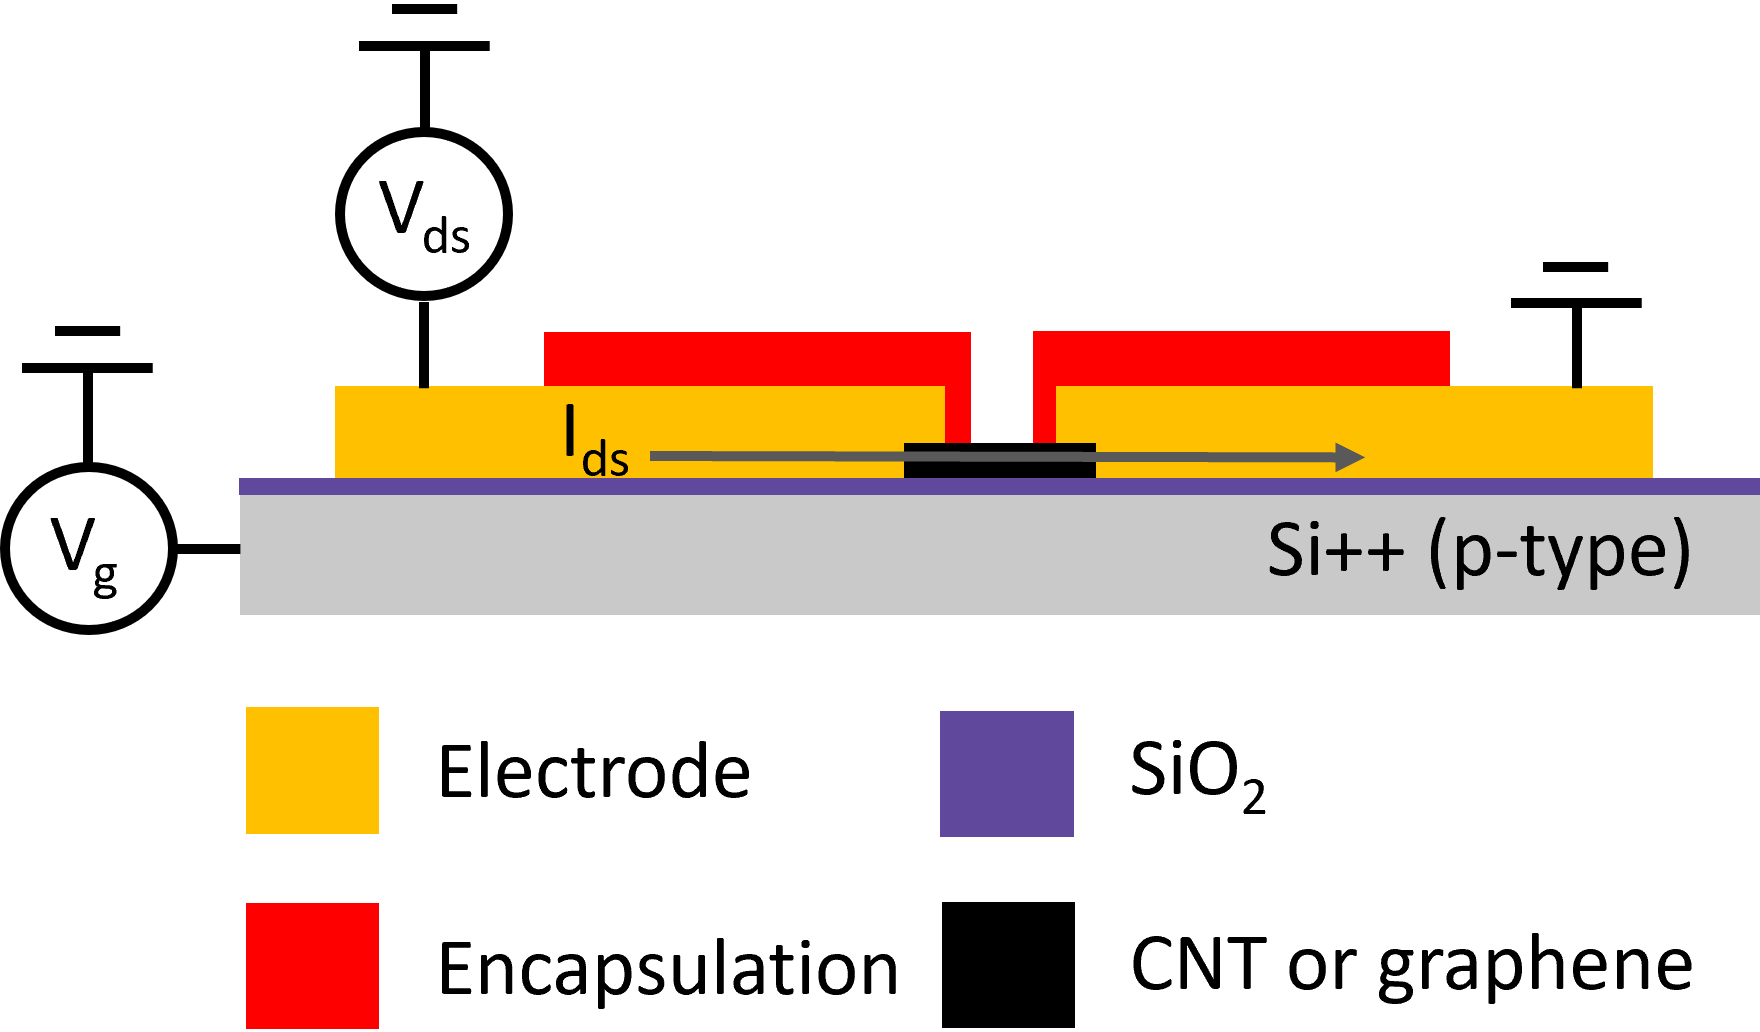
\includegraphics{figures/ch2/back-gate-schematic.png}

}

}

\end{minipage}%
%
\begin{minipage}[t]{0.01\linewidth}

{\centering 

~

}

\end{minipage}%
%
\begin{minipage}[t]{0.03\linewidth}

{\centering 

\raisebox{-\height}{

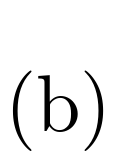
\includegraphics{figures/(b).png}

}

}

\end{minipage}%
%
\begin{minipage}[t]{0.01\linewidth}

{\centering 

~

}

\end{minipage}%
%
\begin{minipage}[t]{0.45\linewidth}

{\centering 

\raisebox{-\height}{

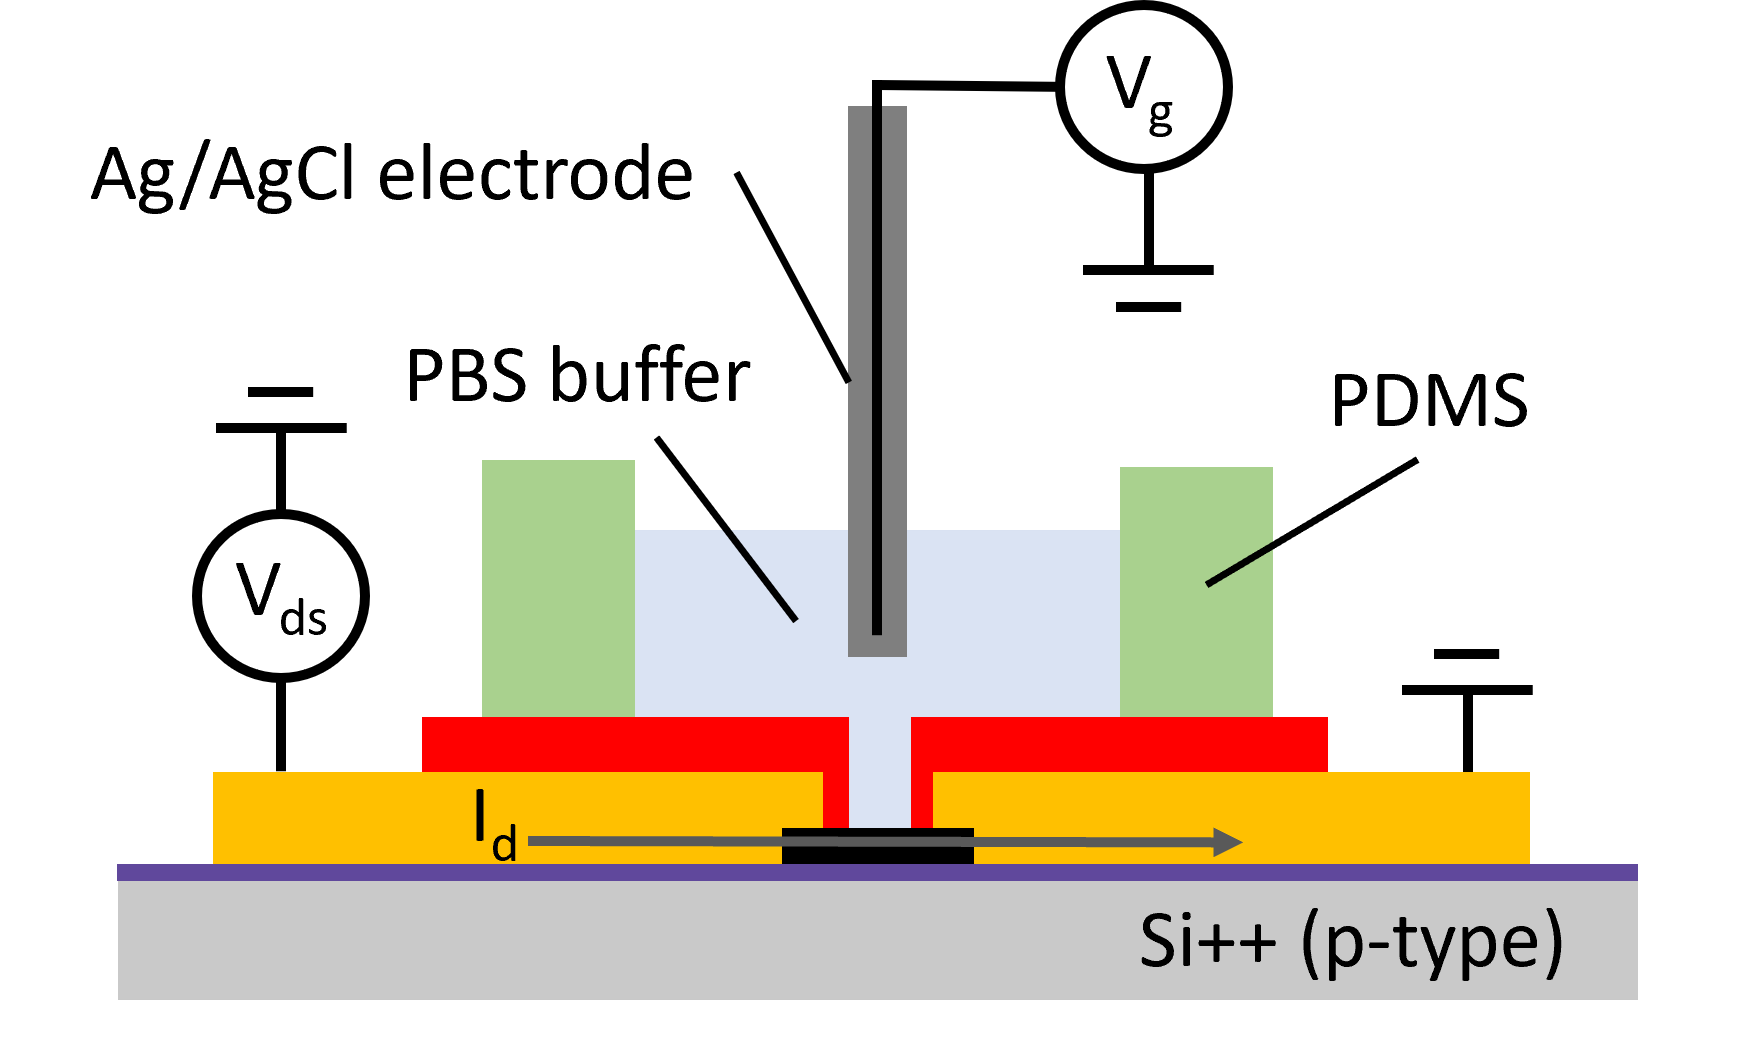
\includegraphics{figures/ch2/liquid-gate-schematic.png}

}

}

\end{minipage}%
%
\begin{minipage}[t]{0.01\linewidth}

{\centering 

~

}

\end{minipage}%

\caption{\label{fig-gating-schematics}Schematics (not to scale) showing
the side-view cross-section of a thin-film field-effect transistor in
both the (a) back-gated and (b) liquid-gated configuration. Here, a
graphene monolayer or a carbon nanotube network is used as the
transistor thin-film. The drain electrode is the gold contact on the
left side of each figure, while the source electrode is the gold contact
on the right.}

\end{figure}

Two basic configurations of the thin-film transistor are the back-gated
field-effect transistor and the liquid-gated (or electrolyte-gated)
transistor. The relatively simple back-gated configuration, shown in
Figure~\ref{fig-gating-schematics} (a), uses the degenerately doped Si
substrate as the gate. The channel is isolated from the gate with a thin
SiO\(_2\) layer. A liquid-gated device, shown in
Figure~\ref{fig-gating-schematics} (b), is used for sensitive
liquid-phase analyte detection. A submerged Ag/AgCl reference electrode
is generally used as a top-gate in this configuration. The channel is
isolated from the gate by the bulk of an electrolyte solution, which can
be restricted to the channel area using a hydrophobic
polydimethylsiloxane microchamber or `PDMS well'. The electrolyte used
is typically the biofriendly phosphate-buffered saline (PBS), but other
aqueous salt solutions, polymers and ion-gels have also been used
\autocite{Avouris2007,Shkodra2021,Tran2016,Li2023}. Transistor operation
is controlled by a `drain' bias \(V_{ds}\), placed between the drain and
source electrodes, and a `gate' bias \(V_g\), placed between the gate
and source electrodes. Gate capacitance determines the influence of
\(V_g\) on drain-source current \(I_d\). In general, gate capacitance is
a series combination of geometric capacitance, \(C_{G}\), and the
quantum capacitance\footnote{Quantum or electrochemical capacitance is
  the change in charge with respect to the electrochemical potential of
  a system. The quantum capacitance must be placed in series with the
  geometric capacitance for low density-of-states systems, such as 2D
  nanomaterials \autocite{Luryi1988,Xia2009,Miranda2016}.} of the
channel nanomaterial, \(C_{Q}\)
\autocite{Avouris2007,Cao2009,Heller2009a,Tran2016,Kireev2017,Li2023}.

\hypertarget{liquid-gating-and-debye-length}{%
\subsubsection*{Liquid-Gating and Debye
Length}\label{liquid-gating-and-debye-length}}
\addcontentsline{toc}{subsubsection}{Liquid-Gating and Debye Length}

Understanding the ionic behaviour of the gate electrolyte used in a
liquid-gated device setup gives insight into the gating and sensing
behaviour of the setup. When a voltage is applied at the liquid-gate,
the charged ions in solution move to form two electric double layers,
one at the interface between the electrolyte and gate electrode, and one
at the interface between electrolyte and semiconducting channel, as
shown in Figure~\ref{fig-Debye-length}. The gate capacitance is a series
combination of the capacitance of each EDL in series with quantum
capacitance \(C_{Q}\) \autocite{Heller2010,Kireev2017,Shkodra2021}. The
Gouy-Chapman-Stern model splits the EDL into two distinct regions, the
first being a compact layer of ions, the Stern layer, and the second
being a more diffuse layer, the Gouy-Chapman layer
\autocite{Tiwari2022}. The surface potential of the solid-electrolyte
interface exponentially decreases across the diffuse region of the
double-layer; the characteristic length of this potential screening is
known as Debye length, \(\lambda_D\). The typical electrolyte Debye
length is on a nanometer scale, therefore the bulk electrolyte acts as
an insulator, similar to the SiO\(_2\) dielectric in the back-gated
configuration. The Stern layer capacitance is inversely proportional to
the Debye length, and therefore decreased \(\lambda_D\) corresponds to
increased gate capacitance
\autocite{Heller2010,Ohno2015,Shkodra2021,Yao2021}.

\begin{figure}

{\centering 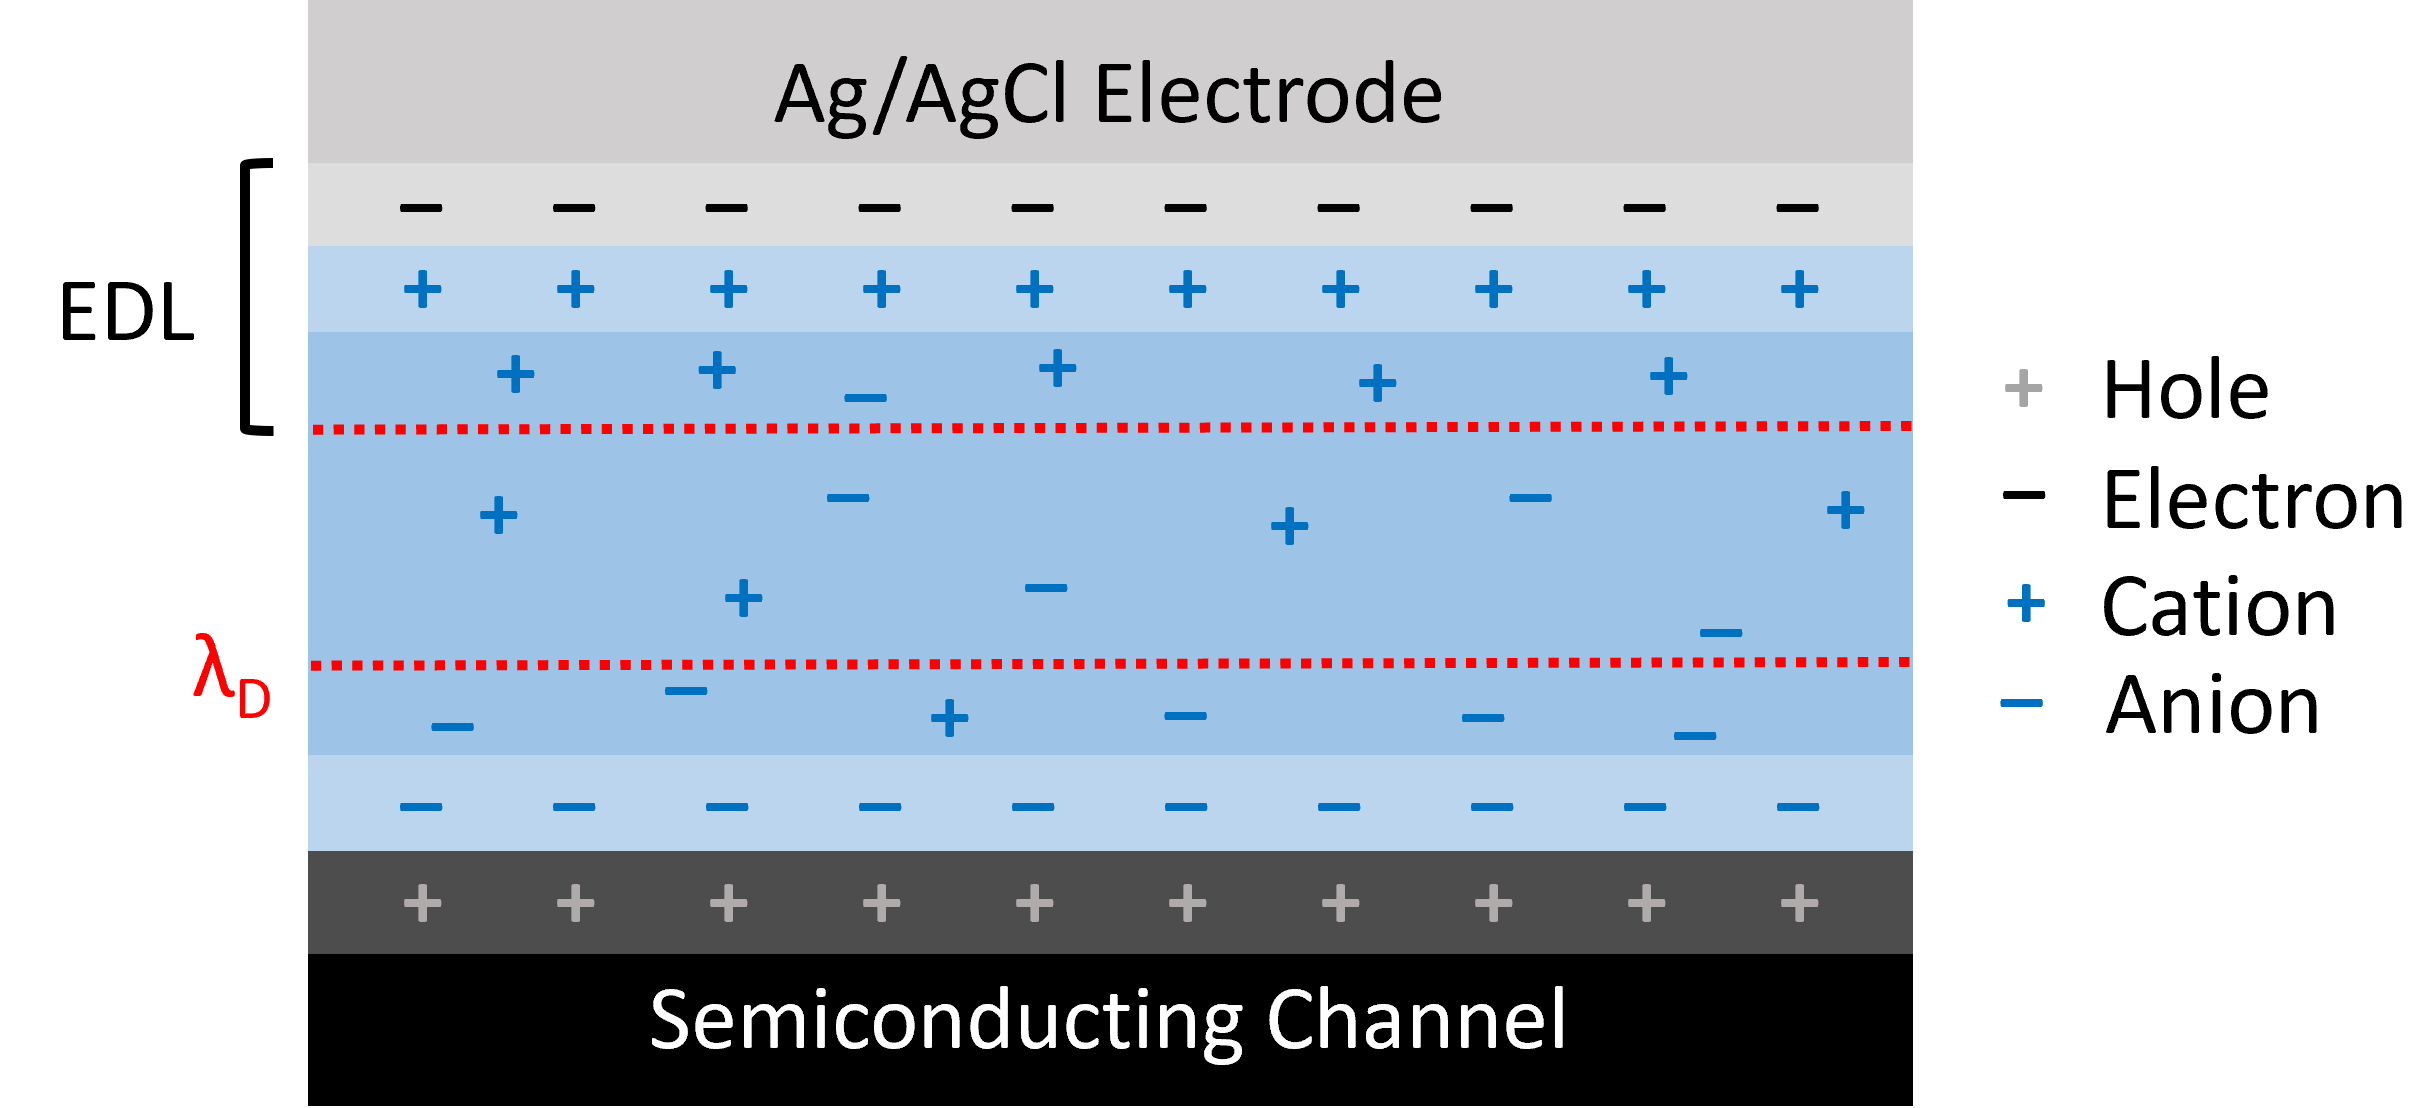
\includegraphics[width=0.7\textwidth,height=\textheight]{figures/ch2/Debye-length-schematic-alt.png}

}

\caption{\label{fig-Debye-length}A diagram of the formation of an
electric double layer (EDL) under an applied voltage between source and
liquid-gate electrodes, with a \(p\)-type semiconductor used for the
channel thin-film. Electric double layers are present at both the
gate-electrolyte interface and semiconductor-electrolyte interface.
Adapted from \autocite{Ohno2015,Shkodra2021,Tiwari2022}.}

\end{figure}

The equation for Debye length \(\lambda_D\) in an electrolyte solution
is given by Equation~\ref{eq-debye-length}.

\begin{equation}\protect\hypertarget{eq-debye-length}{}{
\lambda_D = \sqrt{\frac{\epsilon_0\epsilon_rk_bT}{2N_Aq^2I}}
}\label{eq-debye-length}\end{equation}

Here, \(\epsilon_0\) is vacuum permittivity, \(\epsilon_r\) is the
relative permittivity of the electrolyte, \(\k_B\) is the Boltzmann
constant, \(T\) is absolute temperature in K, \(N_A\) is the Avogadro
number, \(q\) is the elementary charge and \(I\) is ionic strength in
mmol L\(^{-1}\). When temperature is kept constant, \(\lambda_D\) only
depends on the ionic strength of the electrolyte and not on any
attributes of the gate electrode or channel
\autocite{Stern2007,Shkodra2021}. Successive dilutions of a particular
electrolyte will increase the Debye length: for \(1 \times\) PBS,
\(\lambda_D\) is \(\sim\) 1 nm, for \(0.1 \times\) PBS, \(\lambda_D\) is
\(\sim\) 2 nm, for \(0.01 \times\) PBS \(\lambda_D\) is \(\sim\) 8 nm
and so on. This means gate capacitance is directly dependent on the
electrolyte used and its concentration
\autocite{Kireev2017,Shkodra2021}. A \(1 \times\) PBS electrolyte gives
a gate capacitance several orders of magnitude larger than that of a
SiO\(_2\) back-gate. A larger capacitance significantly increases the
effect of electrostatic gating on the channel current, often described
as increased electrostatic coupling between gate and channel. A
liquid-gated device with low Debye length will therefore be highly
sensitive to electrostatic changes across a small voltage range
\autocite{Heller2010,Ohno2015,Kireev2017,Yao2021}.

However, a decreased Debye length also has disadvantages for sensing.
Electrostatic potentials outside of the electrolyte-channel electrical
double layer are effectively screened from the channel. Electrical
double layers will also form around charged receptors within the
solution. The combined screening effect means signals due to potential
changes in charged biomolecules within the bulk electrolyte will have no
effect on gating of the channel, and therefore no effect on \(I_d\).
Interactions between the analyte and any receptor element must therefore
occur within the Debye length, and so a tradeoff exists between channel
sensitivity and the size of the sensitive region above the channel. Many
medium or large proteins will require a relatively dilute electrolyte
for analyte capture to be detected by the channel, which may not reflect
the intended environment for biosensor application
\autocite{Stern2007,Piccinini2018,Shkodra2021}. Other approaches to
increasing Debye length without reducing device sensitivity have
therefore also been trialled. One approach involves attaching a layer of
polyethylene glycol polymer (PEG) to the channel, limiting the approach
of counterions. This increases Debye length at the electrolyte-channel
interface while preserving the capacitance of the electrolyte-gate
interface, keeping device sensitivity relatively high
\autocite{Gao2016,Filipiak2018,Kesler2020,Albarghouthi2022}.

\hypertarget{electrical-characterisation}{%
\subsection{Electrical
Characterisation}\label{electrical-characterisation}}

\begin{figure}

{\centering 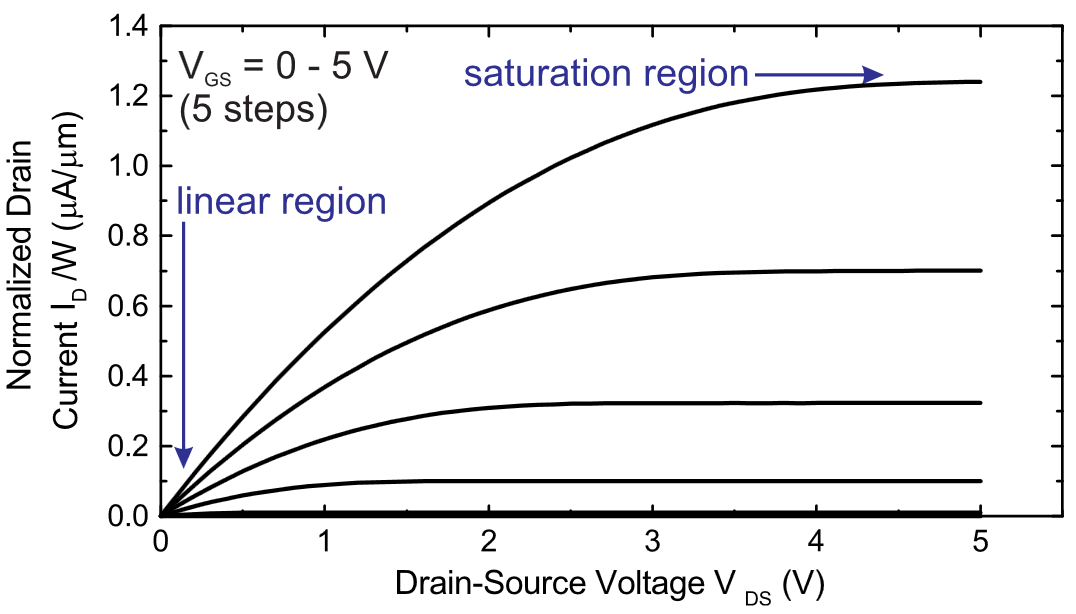
\includegraphics[width=0.65\textwidth,height=\textheight]{figures/ch2/linear_region_edit.png}

}

\caption{\label{fig-linear-region}The linear and saturation operation
regimes of an \(n\)-type metal oxide semiconductor TFT, \(V_{t} \sim 0\)
V. Current has been normalised with respect to channel width (W).
Reproduced with permission from \autocite{Petti2016}.}

\end{figure}

The current-voltage plots of a given transistor are known as its
`characteristic curves'. The I-V curve of \(I_d\) against \(V_{ds}\) at
constant \(V_g\) is known as the `source-drain' or `output'
characteristic curve, while \(I_d\) against \(V_g\) at constant
\(V_{ds}\) is known as the `transfer' characteristic curve at that
source-drain voltage \autocite{Kauffman2008,Petti2016,Shkodra2021}.
Applying a gate voltage \(V_g\) to the gate of an thin-film transistor
influences the amount and type of available charge carriers for
conduction \autocite{Avouris2007,Tran2016,Heller2009a}. In an ambipolar
transistor, a highly negative \(V_g\) will give rise to hole conduction,
and a highly positive \(V_g\) will give rise to electron conduction
\autocite{Avouris2007,Yao2021,Li2023}. The minimum \(V_g\) required to
turn the flow of current in a thin-film transistor `on' is referred to
as the threshold voltage \(V_t\)
\autocite{Petti2016,Shkodra2021,Li2023}. Threshold voltage is discussed
in more detail in Section~\ref{sec-electrical-characterisation-CNT}.
When \(|V_{ds}| < |V_g| - |V_t|\) while \(|V_g|>|V_t|\), the device is
in the linear regime. Here, \(V_{ds}\) is directly proportional to
\(I_{d}\), similar to an Ohmic resistor. When
\(|V_{ds}| > |V_g| - |V_t|\) and \(|V_g|>|V_t|\), the device is in the
saturation regime, where the relationship between \(V_{ds}\) and
\(I_{d}\) becomes non-linear \autocite{Petti2016,Shkodra2021,Li2023}.

\begin{figure}

\begin{minipage}[t]{0.03\linewidth}

{\centering 

\raisebox{-\height}{


\includegraphics{figures/(a).png}

}

}

\end{minipage}%
%
\begin{minipage}[t]{0.01\linewidth}

{\centering 

~

}

\end{minipage}%
%
\begin{minipage}[t]{0.45\linewidth}

{\centering 

\raisebox{-\height}{

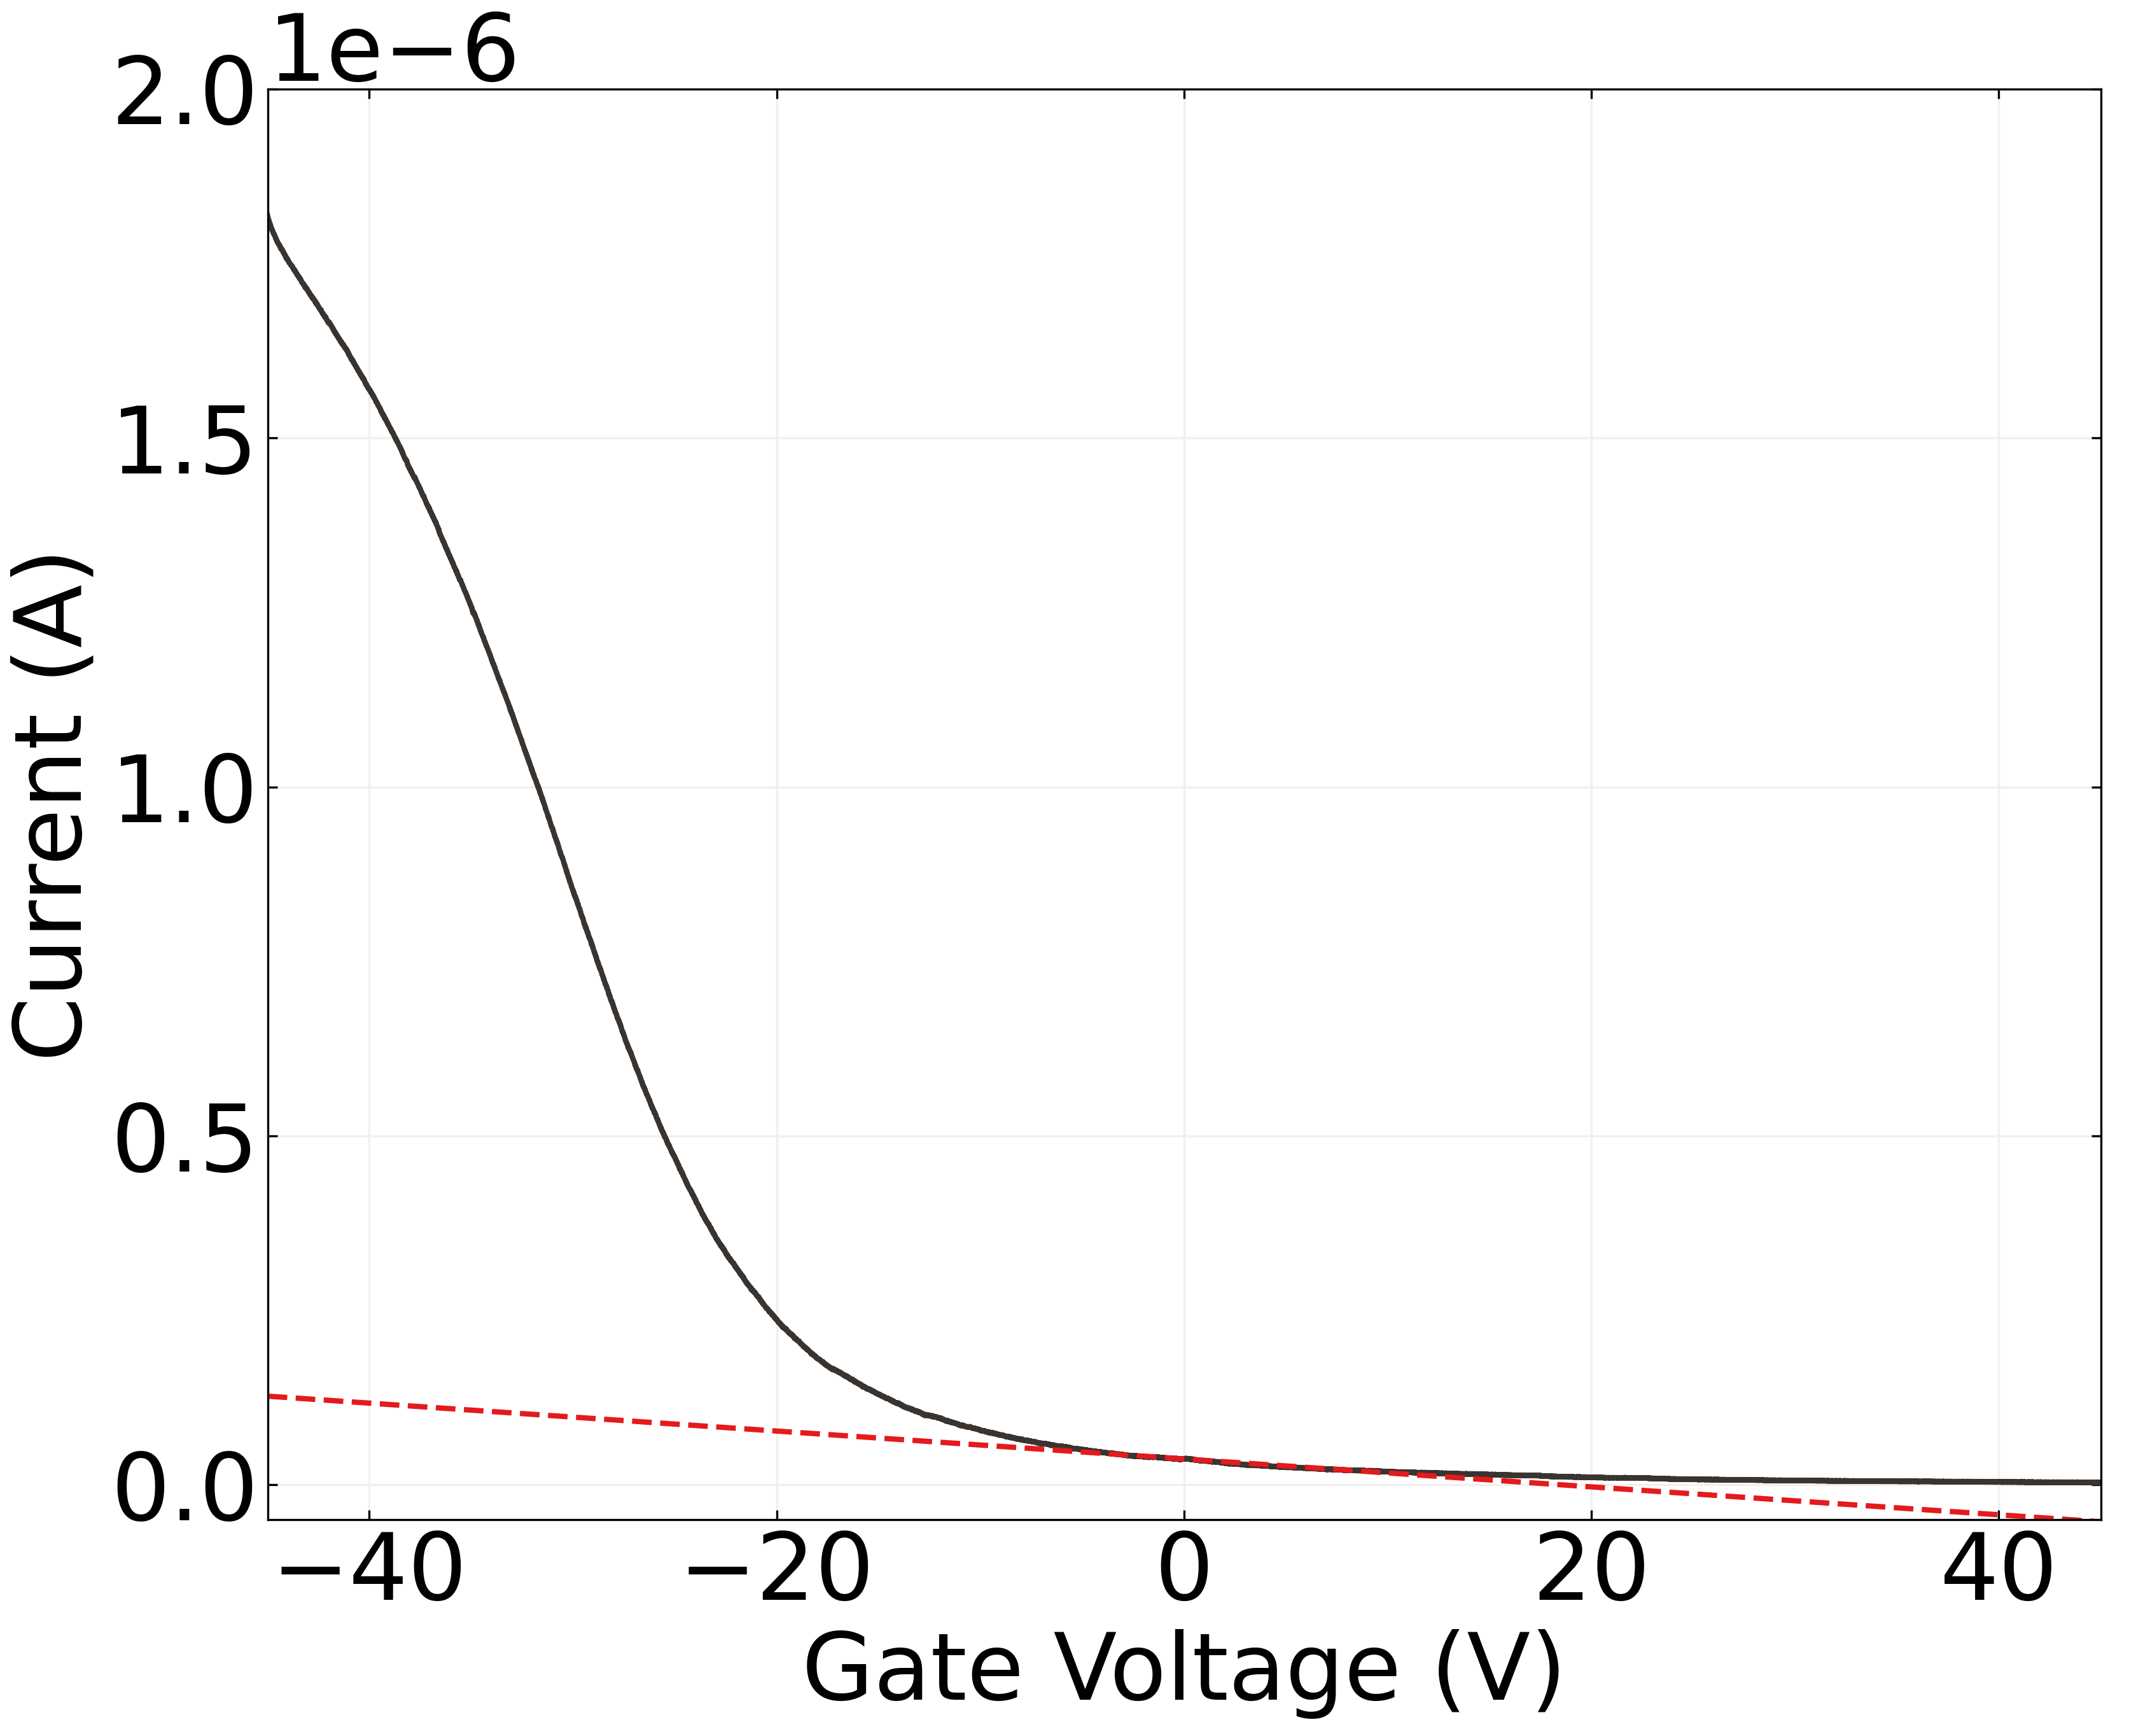
\includegraphics{figures/ch2/Q5C10ch8transconductance.png}

}

}

\end{minipage}%
%
\begin{minipage}[t]{0.01\linewidth}

{\centering 

~

}

\end{minipage}%
%
\begin{minipage}[t]{0.03\linewidth}

{\centering 

\raisebox{-\height}{

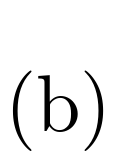
\includegraphics{figures/(b).png}

}

}

\end{minipage}%
%
\begin{minipage}[t]{0.01\linewidth}

{\centering 

~

}

\end{minipage}%
%
\begin{minipage}[t]{0.45\linewidth}

{\centering 

\raisebox{-\height}{

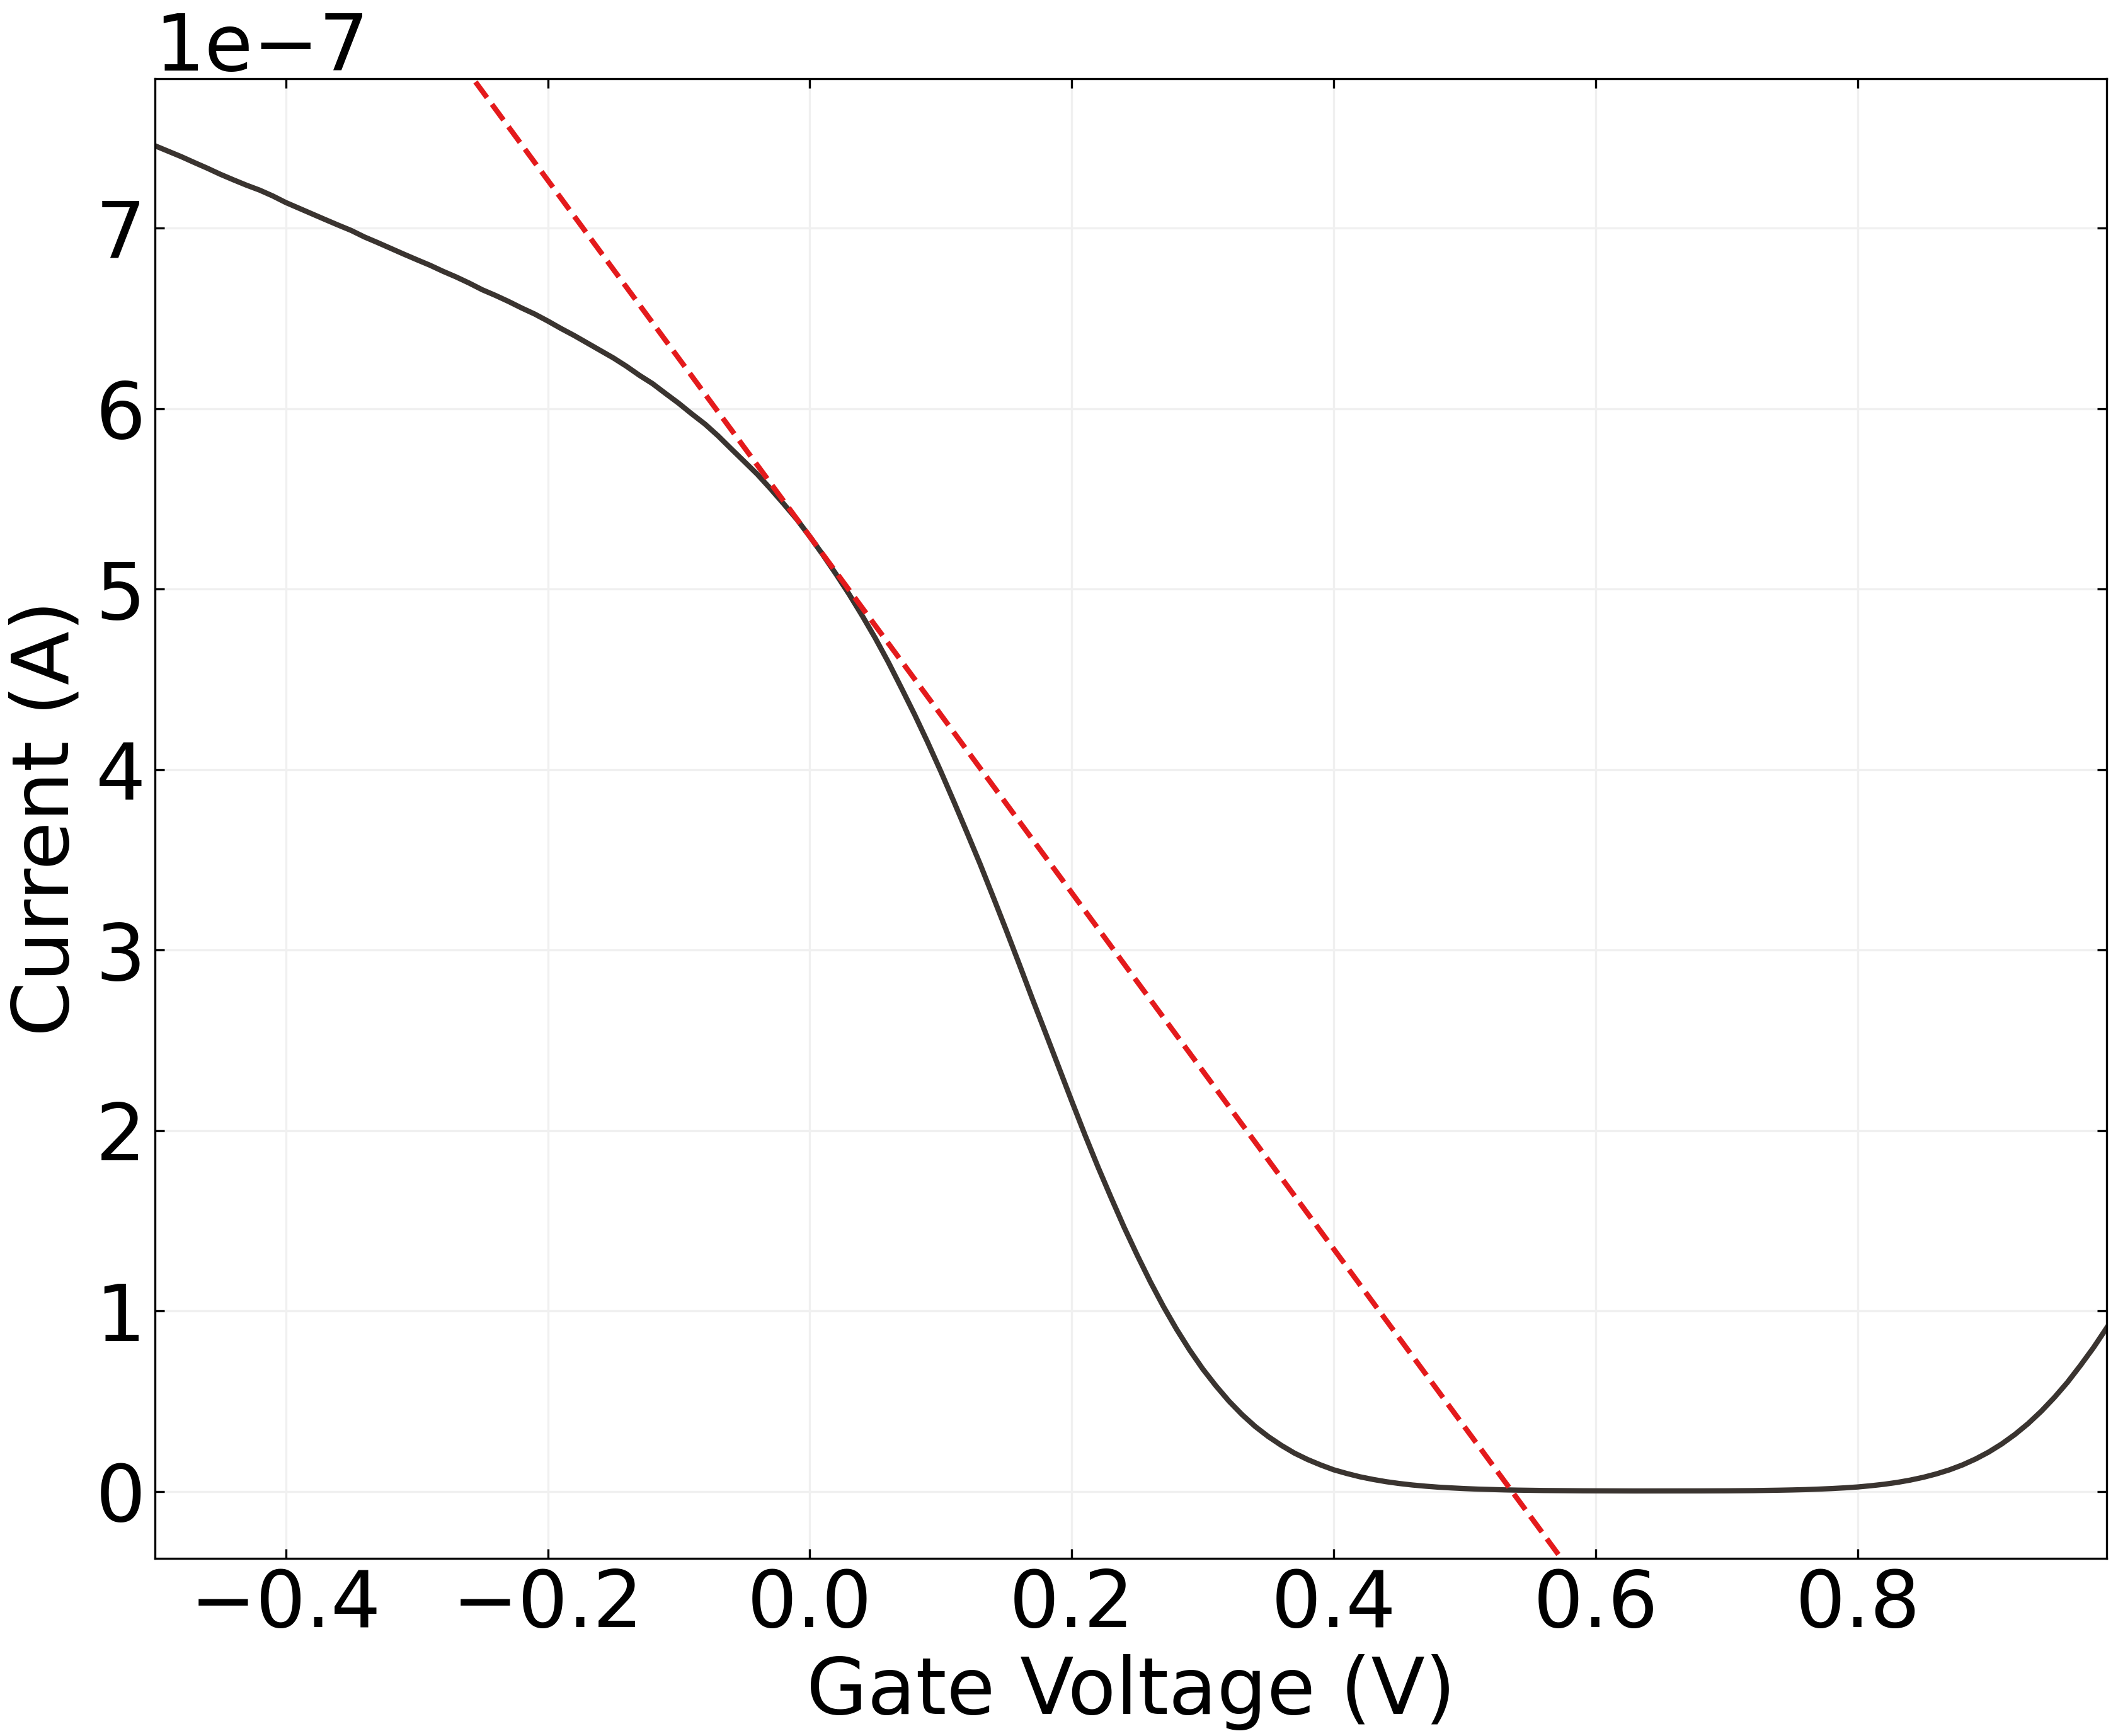
\includegraphics{figures/ch2/NTQ31C5ch1transconductance.png}

}

}

\end{minipage}%
%
\begin{minipage}[t]{0.01\linewidth}

{\centering 

~

}

\end{minipage}%
\newline
\begin{minipage}[t]{0.03\linewidth}

{\centering 

\raisebox{-\height}{


\includegraphics{figures/(c).png}

}

}

\end{minipage}%
%
\begin{minipage}[t]{0.01\linewidth}

{\centering 

~

}

\end{minipage}%
%
\begin{minipage}[t]{0.45\linewidth}

{\centering 

\raisebox{-\height}{

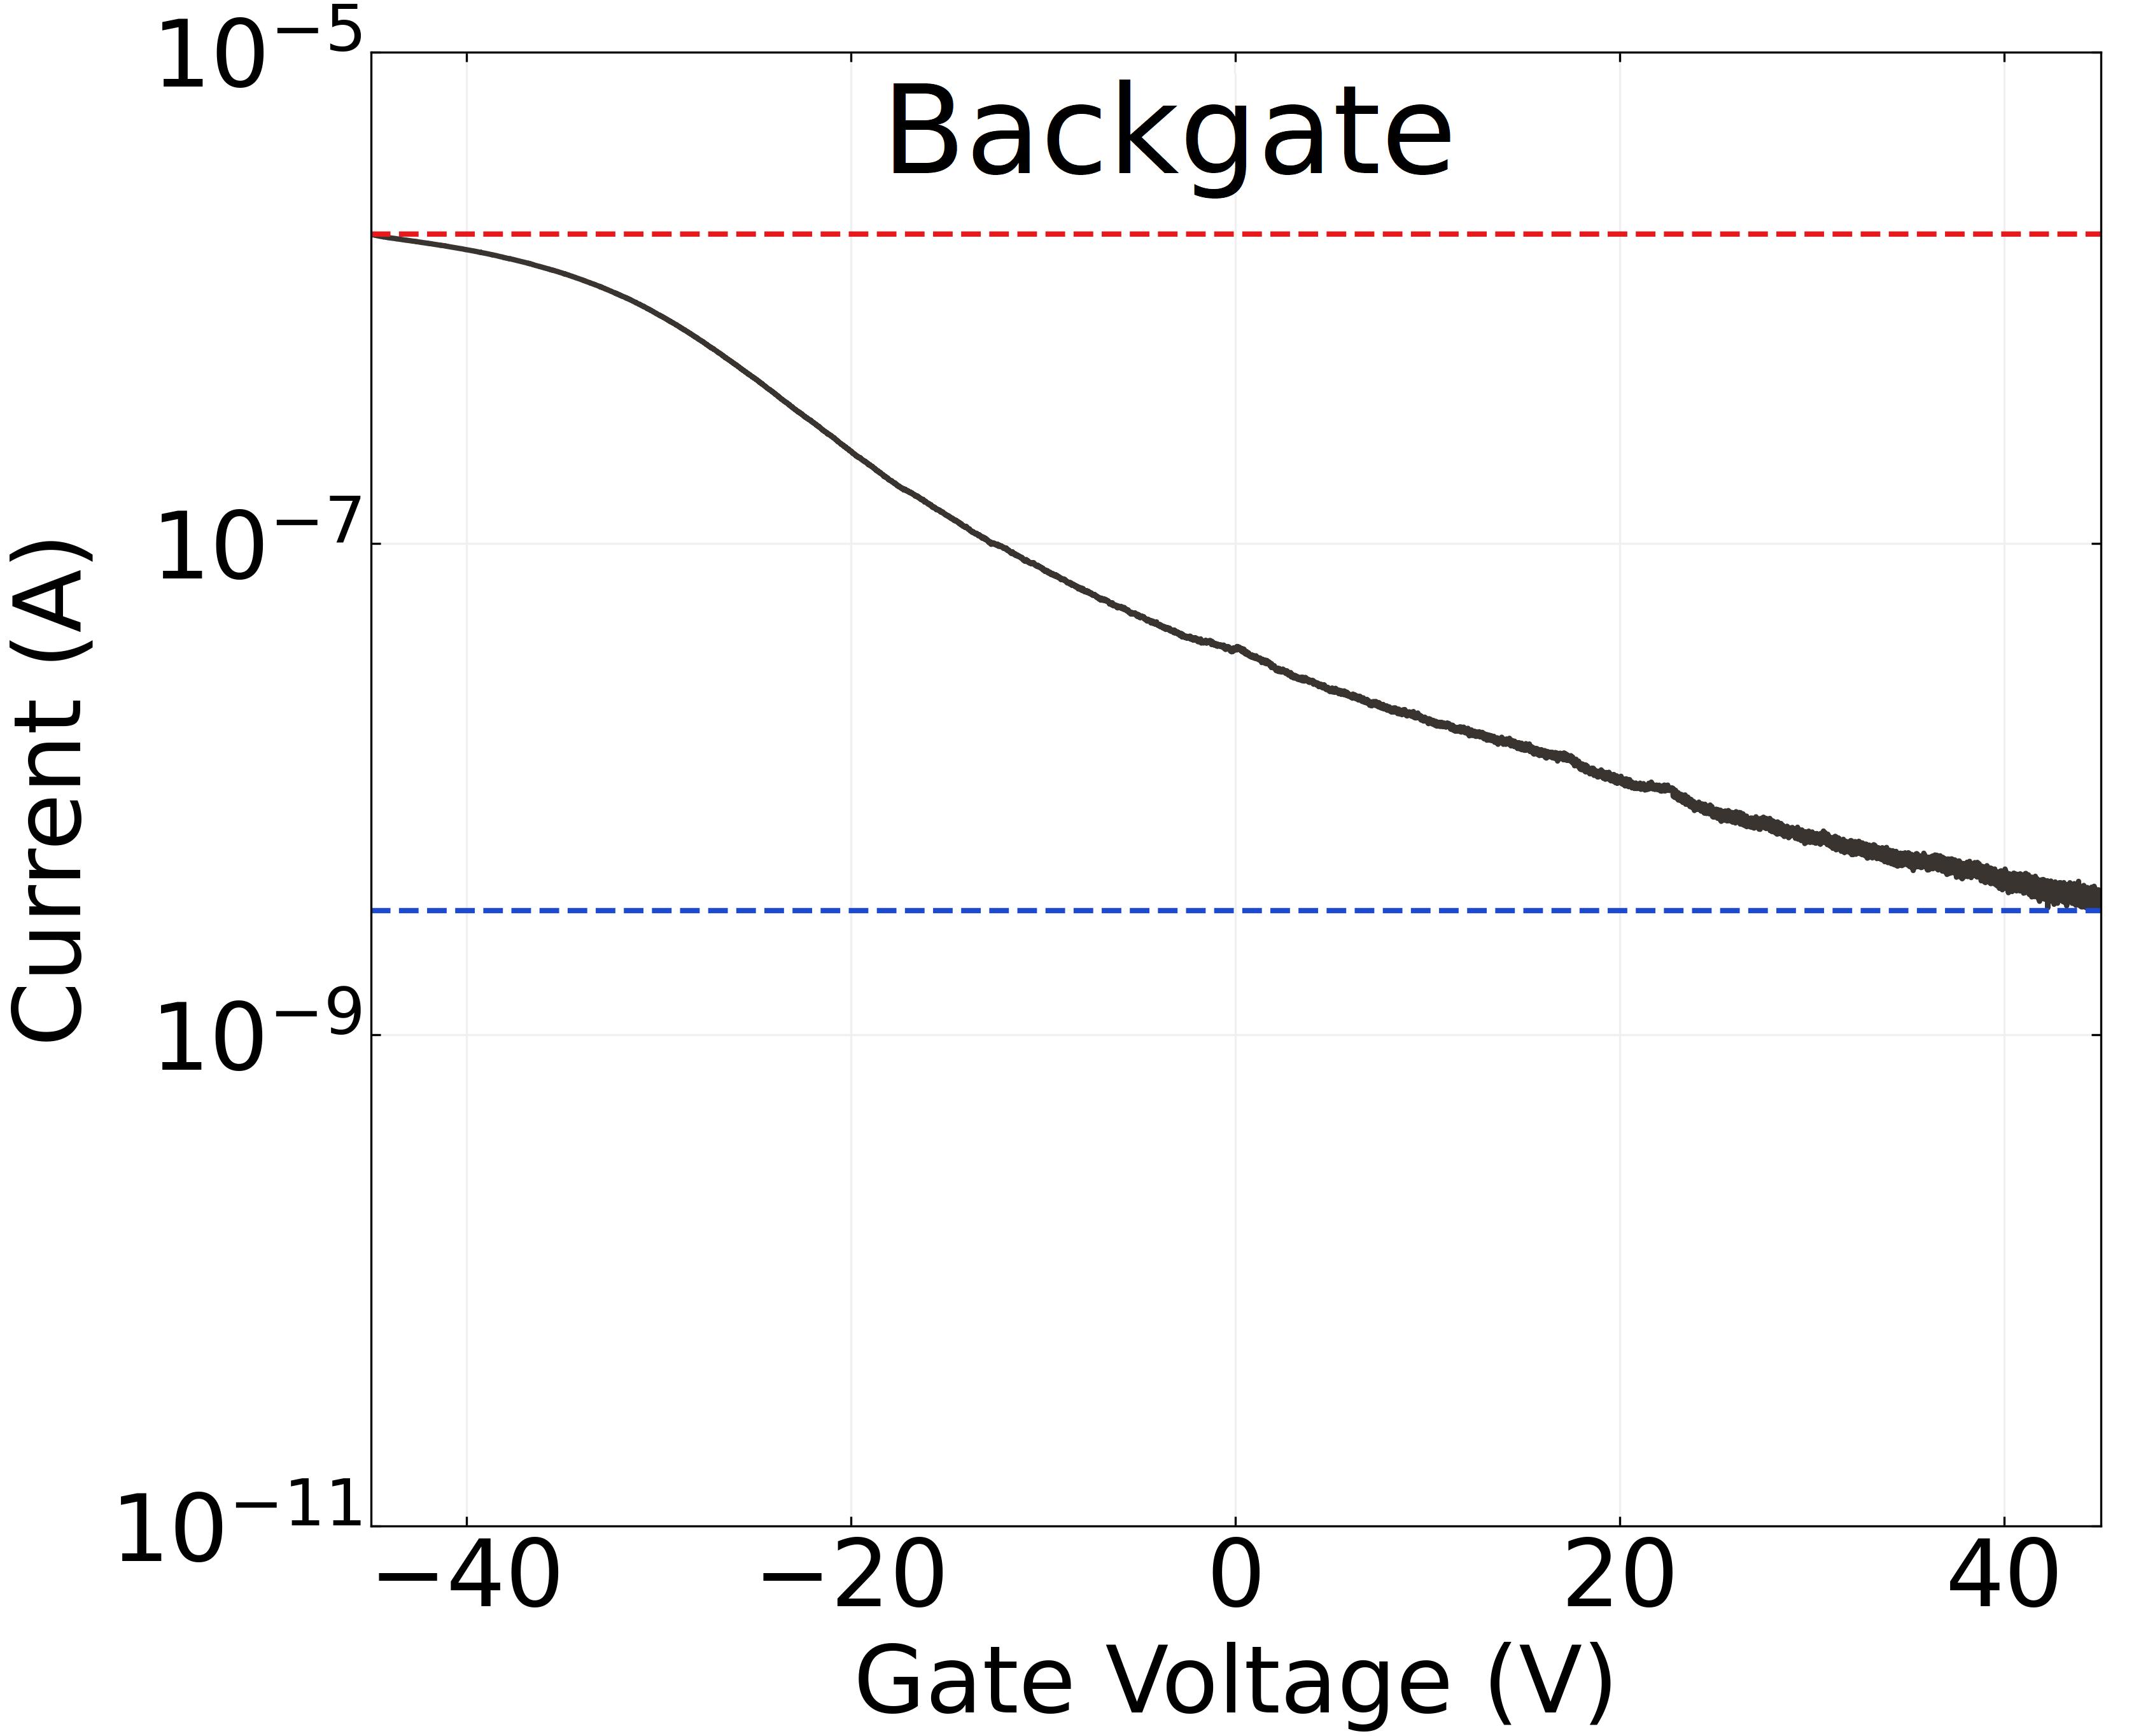
\includegraphics{figures/ch2/Q5C10ch8on_off_current.png}

}

}

\end{minipage}%
%
\begin{minipage}[t]{0.01\linewidth}

{\centering 

~

}

\end{minipage}%
%
\begin{minipage}[t]{0.03\linewidth}

{\centering 

\raisebox{-\height}{

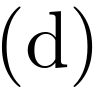
\includegraphics{figures/(d).png}

}

}

\end{minipage}%
%
\begin{minipage}[t]{0.01\linewidth}

{\centering 

~

}

\end{minipage}%
%
\begin{minipage}[t]{0.45\linewidth}

{\centering 

\raisebox{-\height}{

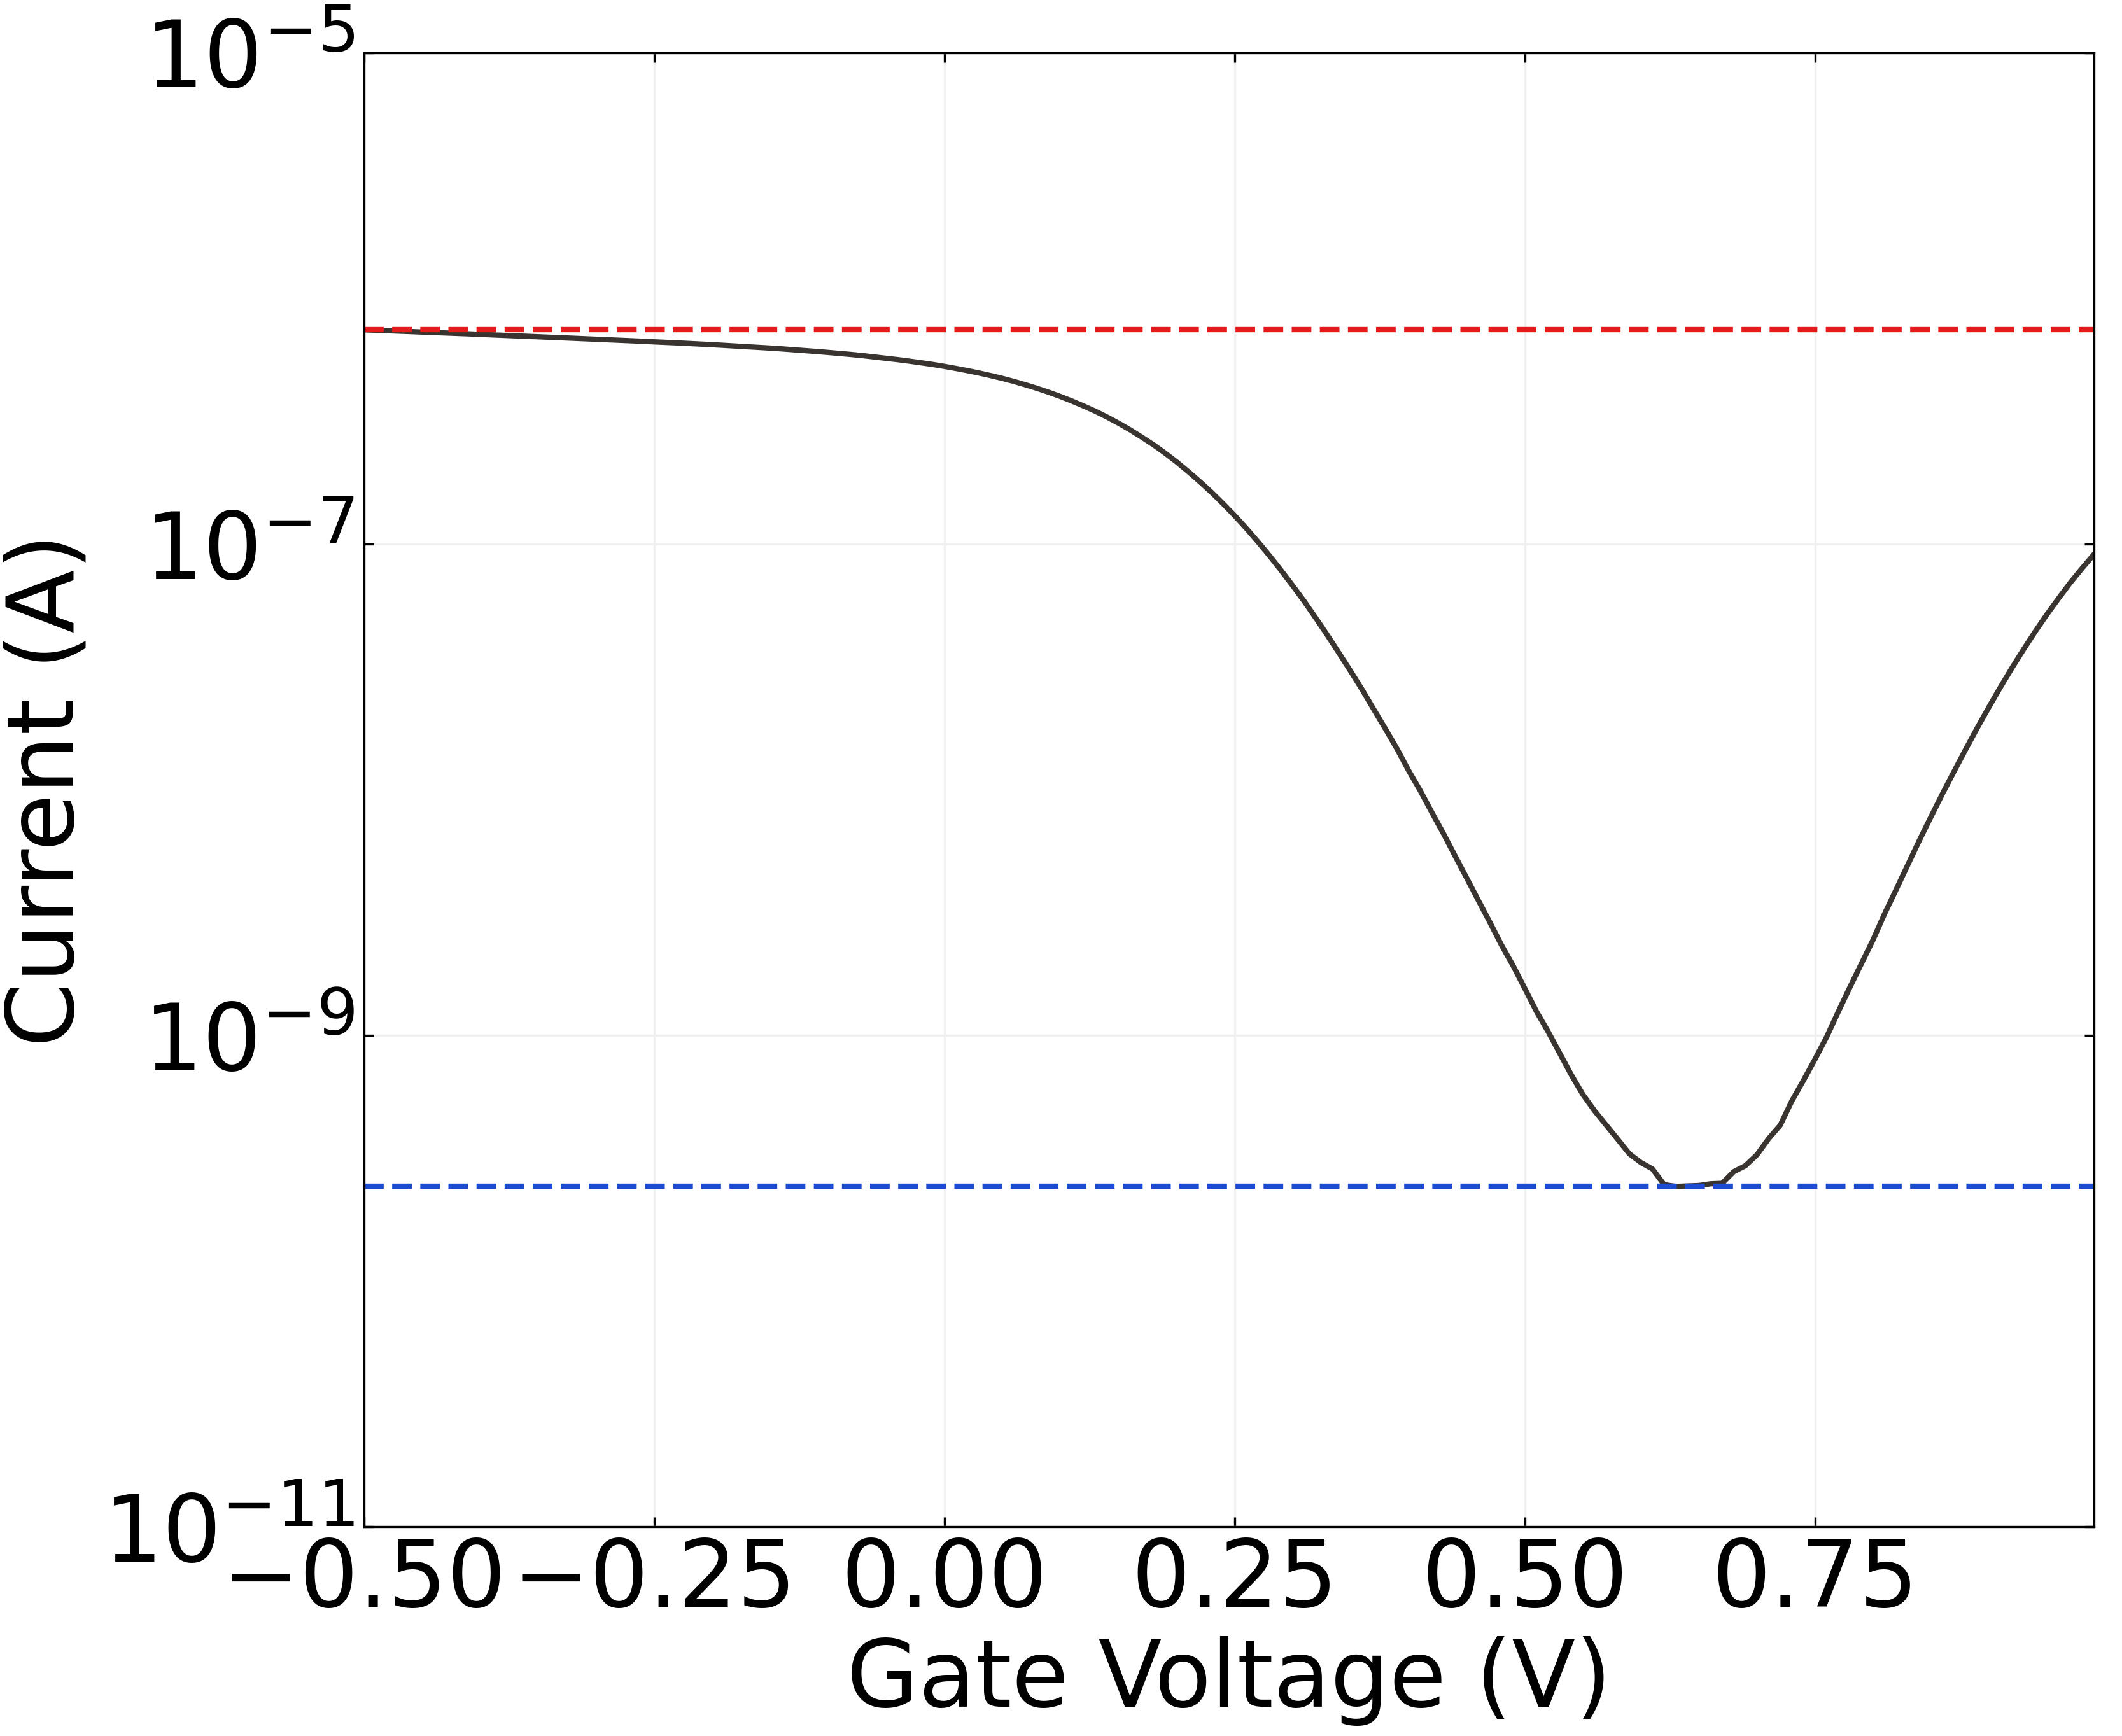
\includegraphics{figures/ch2/NTQ31C5ch1on_off_current.png}

}

}

\end{minipage}%
%
\begin{minipage}[t]{0.01\linewidth}

{\centering 

~

}

\end{minipage}%

\caption{\label{fig-gating-transfer}Examples of field-effect transistor
transfer characteristics taken at \(V_{ds}\) = 100 mV using two carbon
nanotube network device channels fabricated in the same manner. A linear
scale is used in (a) and (b), while a logarithmic scale is used in (c)
and (d). The curves in (a) and (c) are from a backgated channel, while
the curves in (b) and (d) are from a liquid-gated channel. The linear
fit with gradient corresponding to transconductance at \(V_g\) = 0 V is
shown in (a) and (b) with a dotted red line. The approximate on current
in (c) and (d) is shown with a red horizontal line, while the off
current is shown with a blue horizontal line.}

\end{figure}

The linear and saturation regions for a metal oxide thin-film transistor
are shown in Figure~\ref{fig-linear-region}. In this thesis, constant
\(V_g\) measurements from thin-film transistors were typically taken
when \(V_{ds}\) was small and the TFT was in the linear operation
regime. Figure~\ref{fig-gating-transfer} (a) and (c) show back-gated
transfer characteristics of a thin-film transistor, and
Figure~\ref{fig-gating-transfer} (b) and (d) show liquid-gated TFT
transfer characteristics. The back-gated device exhibits unipolar
behaviour, where the transistor conducts in only one direction along the
\(I_d - V_g\) curve, while the liquid-gated device exhibits ambipolar
behaviour, where conduction occurs along both directions of the curve.
The liquid-gated device is also able to traverse a wide range of
currents over a much more limited voltage interval than the back-gated
device. A variety of quantitative parameters or figures of merit can be
extracted from the transfer characteristics of a thin-film transistor
\autocite{Petti2016}. Transconductance and on-off ratio are discussed
below, while threshold voltage and subthreshold swing are discussed for
the carbon nanotube network case in
Section~\ref{sec-electrical-characterisation-CNT}.

One of the most important figures of merit which can be extracted from
the transfer characteristic curve of a thin-film FET is the on-off
current ratio, the ratio of the current through a device when the
transistor is gated fully `on', \(I_{on}\), to the current \(I_{off}\)
when gated fully `off'. \autocite{Kauffman2008,Petti2016,Shkodra2021}.
Having a low off current is desirable as it corresponds to low power
consumption by the transistor \autocite{Rouhi2010}. In
Figure~\ref{fig-gating-transfer} (a), there is a clear on regime at
large negative voltages and an off regime at large positive voltages.
Although the transfer curve never completely flattens in each direction,
\(I_{on}\) can be reasonably estimated with the highest current
obtained, while \(I_{off}\) can be estimated from the lowest current
reading. In an ambipolar FET, such as that shown in
Figure~\ref{fig-gating-transfer} (b), the off current can be defined as
the minimum current during the transfer sweep, where the majority
carrier transitions from being holes to electrons or \emph{vice versa}
\autocite{Petti2016,Zheng2017}. For the backgated channel shown in
Figure~\ref{fig-gating-transfer} (a), the on-off ratio
\(I_{on}/I_{off}\) is \(\sim\) 700, while for the liquid-gated device in
Figure~\ref{fig-gating-transfer} (b), \(I_{on}/I_{off} \sim 3000\).
These values are comparable to those found in the literature
\autocite{Avouris2007,Kauffman2008,Heller2010}. The superior on-off
ratio is a significant advantage of the liquid-gated configuration
\autocite{Shkodra2021}.

In the linear regime, transconductance at a specific gate voltage is
given by \(g_m = |dI_{d}/dV_g|\). Transconductance indicates how
responsive the device is to electrostatic gating at a given gate
voltage. In other words, when \(g_m\) is large, small changes in \(V_g\)
can significantly modulate channel current \(I_d\), which is useful for
sensing \autocite{Heller2009a,Ohno2015,Kireev2017}. Transconductance at
a given gate voltage is also proportional to the mobility (movement) of
charge carriers in the device channel, and therefore depends on the
scattering properties of the material
\autocite{Rouhi2010,Petti2016,Li2023}. The transconductance at a
specific gate voltage can be found from performing a linear fit in a
small region around that voltage on the transfer curve. Linear fits for
transconductance at \(V_g = 0\) V, the operating voltage used for
sensing in this thesis, are shown for a back-gated device in
Figure~\ref{fig-gating-transfer} (a), and a liquid-gated device in
Figure~\ref{fig-gating-transfer} (b). The corresponding transconductance
values of \(g_m\) = 0.002 µS and \(g_m\) = 1 µS respectively. The
difference of several orders of magnitude between back-gated and
liquid-gated transconductance corresponds to the difference of several
orders of magnitude between back and liquid-gated gate capacitance
\autocite{Tran2016,Shkodra2021}. The ability to achieve high
transconductance at relatively low voltage is important for the creation
of low power sensors, which is another advantage of the liquid-gated
setup.

Application of higher voltages to the gate in both the liquid-gate and
back-gate cases can result in significant leakage currents through the
gate. These currents mean that the insulating layer at the gate
producing the capacitive effect no longer acts as an insulator,
adversely affecting transistor behaviour and contributing to sensor
drift that may be mistaken for signal responses to analyte
\autocite{Noyce2019,Shkodra2021,Albarghouthi2022}. In the case of
back-gated devices, gate leakage occurs due to conduction through the
oxide dielectric. If the gate voltage produces an electric field
exceeding the dielectric strength of the oxide, dielectric breakdown can
occur, where the oxide layer no longer acts as an insulator. Breakdown
results from voltage-induced oxygen vacancies in the SiO\(_2\) lattice
forming a conductive path through the insulator \autocite{Padovani2017}.
Irreversible breakdown occured at \(\sim\) 50 V for the back-gated
channel in Figure~\ref{fig-gating-transfer}. In the liquid-gated case,
the electrolyte used determines the appropriate voltage range for
electrical characterisation, since excessive voltages will induce redox
reactions. For water-based electrolytes, gate voltages must be kept
within the \(\pm\) 1 V range \autocite{Wang2010,Ohno2015,Shkodra2021}.
In normal operation, gate current should appear negligible on a linear
scale, as shown in Figure~\ref{fig-gating-hysteresis}.

\begin{figure}

\begin{minipage}[t]{0.03\linewidth}

{\centering 

\raisebox{-\height}{


\includegraphics{figures/(a).png}

}

}

\end{minipage}%
%
\begin{minipage}[t]{0.01\linewidth}

{\centering 

~

}

\end{minipage}%
%
\begin{minipage}[t]{0.45\linewidth}

{\centering 

\raisebox{-\height}{

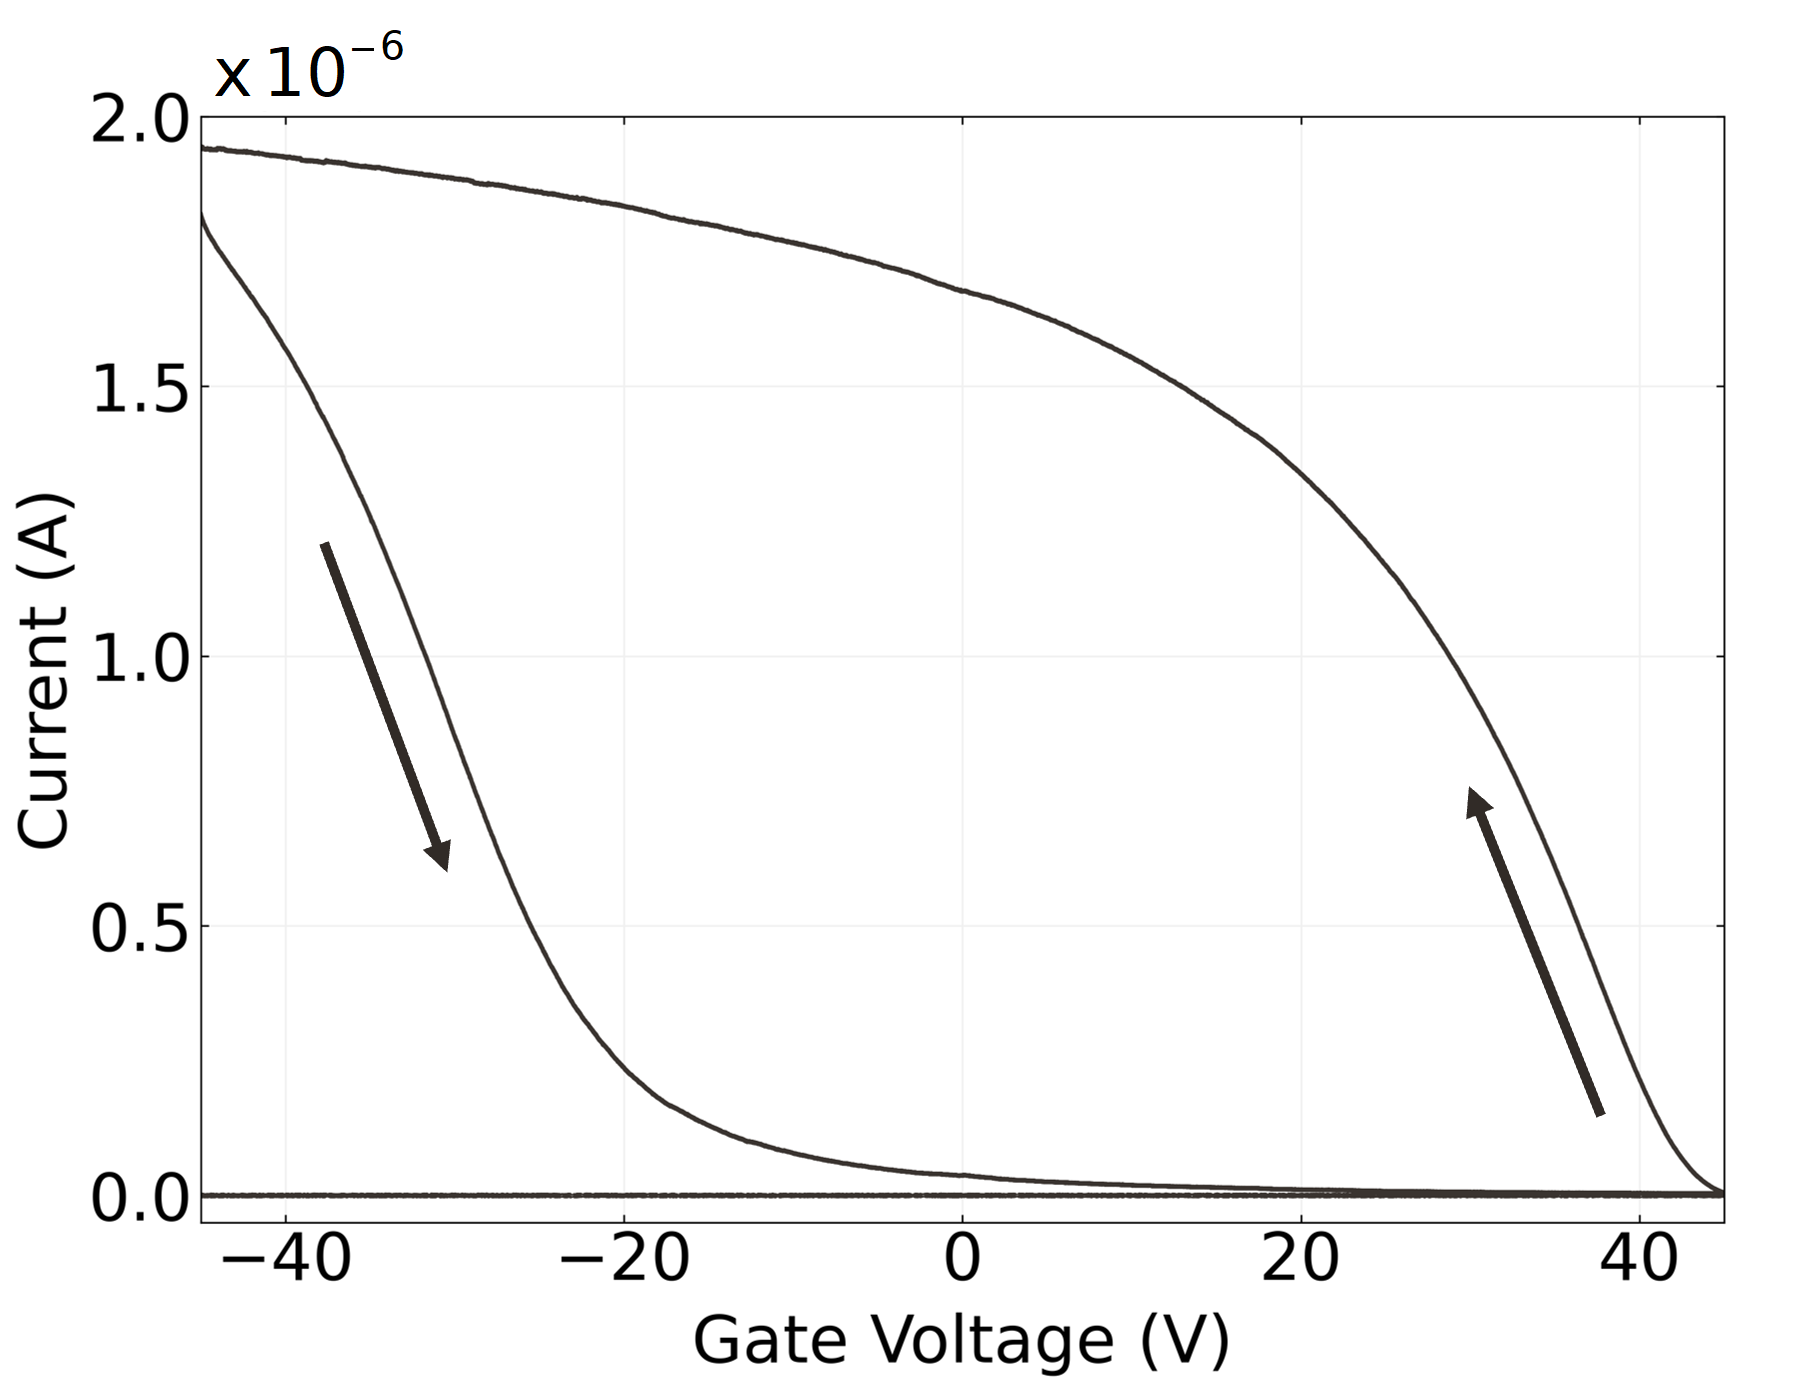
\includegraphics{figures/ch2/Q5C10_hysteresis.png}

}

}

\end{minipage}%
%
\begin{minipage}[t]{0.01\linewidth}

{\centering 

~

}

\end{minipage}%
%
\begin{minipage}[t]{0.03\linewidth}

{\centering 

\raisebox{-\height}{

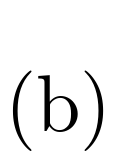
\includegraphics{figures/(b).png}

}

}

\end{minipage}%
%
\begin{minipage}[t]{0.01\linewidth}

{\centering 

~

}

\end{minipage}%
%
\begin{minipage}[t]{0.45\linewidth}

{\centering 

\raisebox{-\height}{

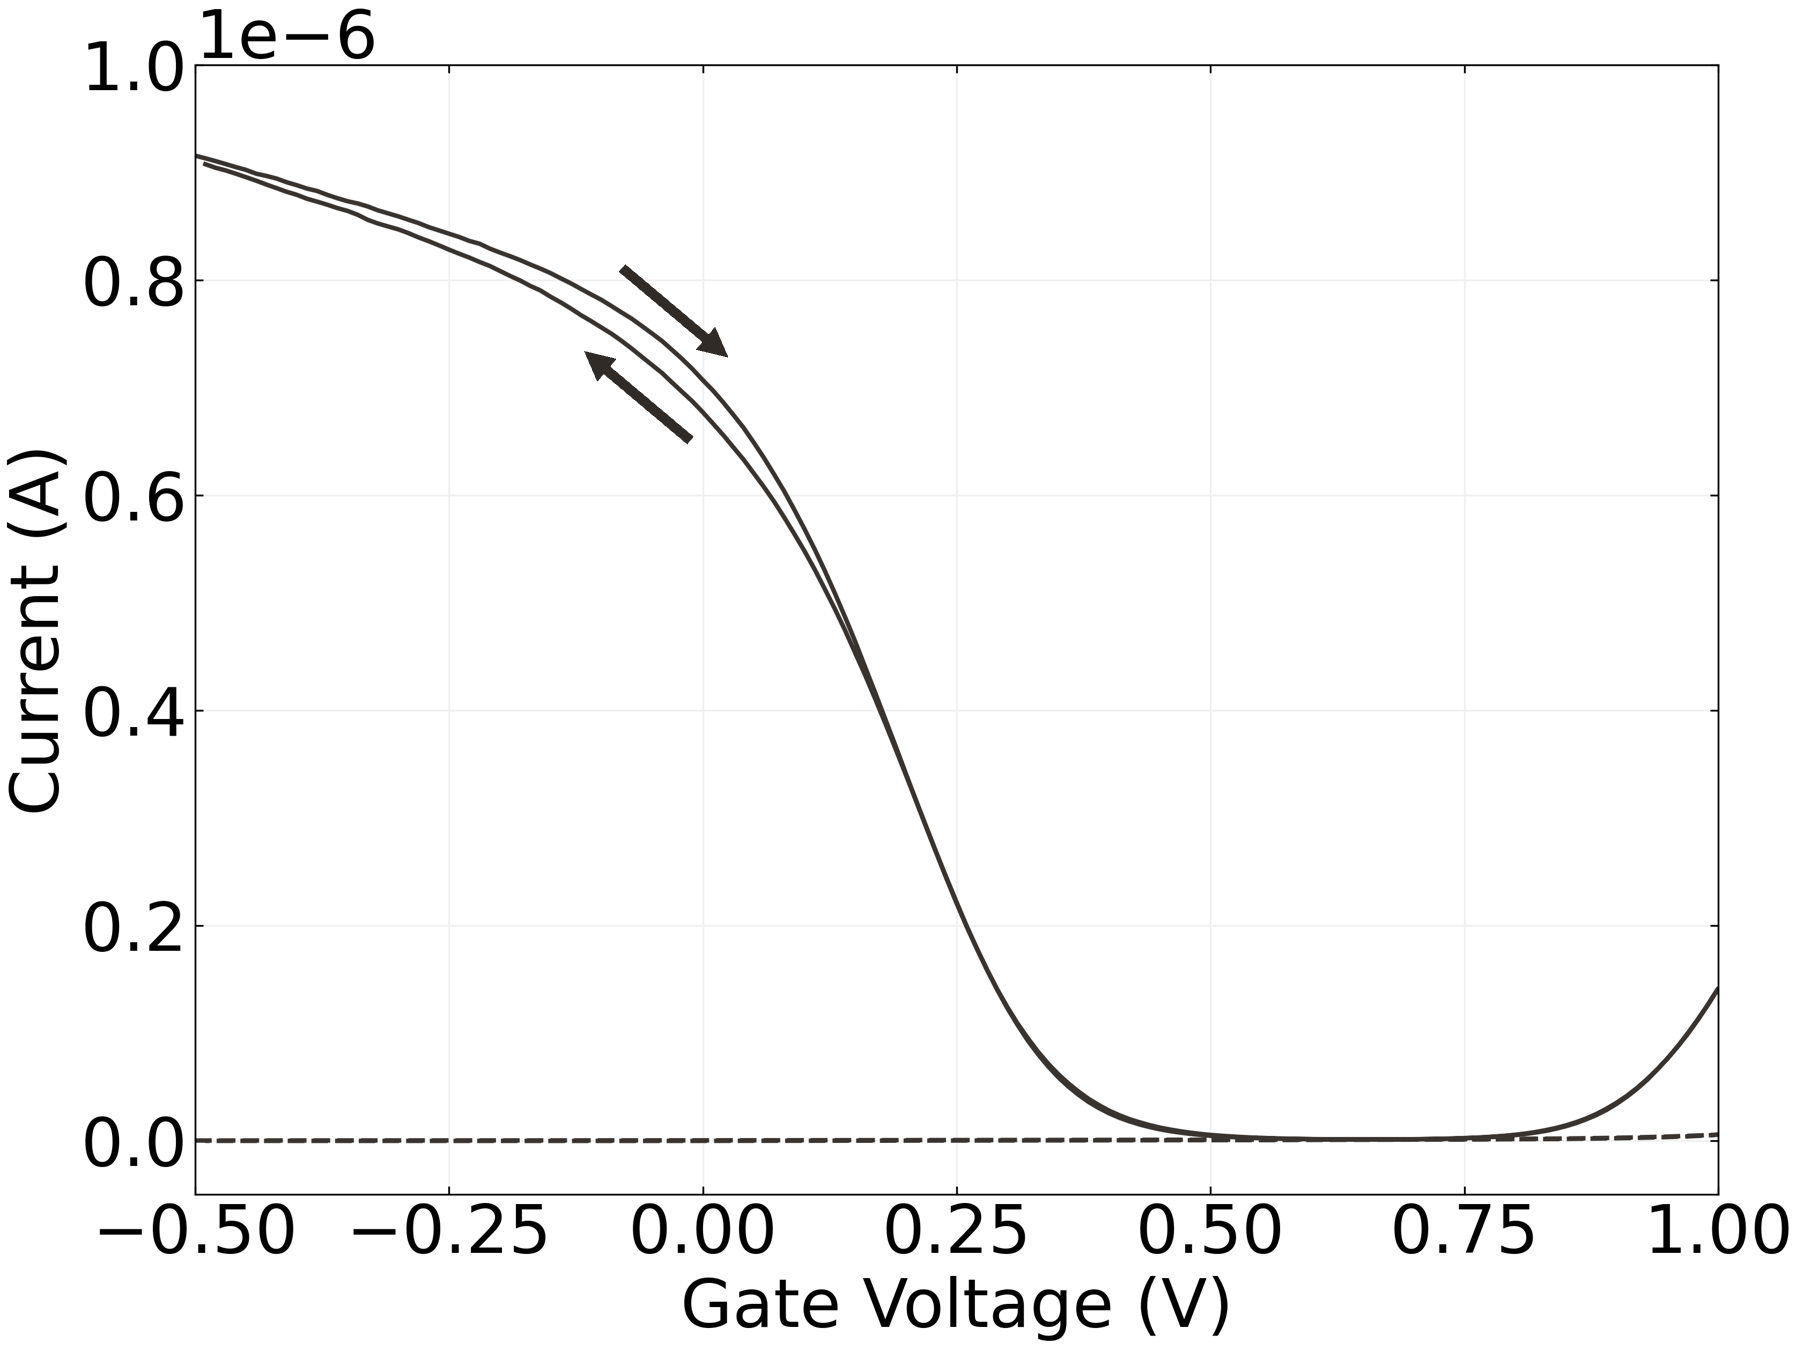
\includegraphics{figures/ch2/NTQ31C5_hysteresis.png}

}

}

\end{minipage}%
%
\begin{minipage}[t]{0.01\linewidth}

{\centering 

~

}

\end{minipage}%

\caption{\label{fig-gating-hysteresis}Field-effect transistor transfer
characteristics taken at \(V_{ds}\) = 100 mV from two different device
channels on a linear scale. Forward and reverse sweeps are shown for the
back-gated case (a) and the liquid-gated case (b), with the direction of
each sweep indicated by an arrow. A sweep rate of \(V_{ds}\) = 10
mV/sample was used for both transfer curves. The gate current measured
during each sweep is also shown with a dotted line.}

\end{figure}

Thin-film transistor devices typically exhibit some degree of
hysteresis, where the history of channel current affects future current
behaviour. Hysteresis in carbon nanotube and graphene field-effect
transistors is a result of filling or emptying of slow-discharge charge
traps in the channel environment. These charge traps effectively dope
the SiO\(_2\) insulator or the insulator-channel interface, which
results from gate bias stress or dopant adsorption
\autocite{McEuen2002,Kim2003,Wang2010,Bartolomeo2011,Bargaoui2018,Peng2018}.
A capacitive gating effect from charged ions also contributes to
hysteresis, from the use of a electrolyte-gated environment or from
charged surface contamination \autocite{Wang2010,Yao2021}. Due to
hysteresis, sweeping \(V_g\) forwards across a set voltage range will
result in a different \(I_d - V_g\) characteristic curve than
subsequently sweeping over \(V_g\) in the reverse direction. Hysteresis
depends on the voltage range used for characterisation, the sweep rate
and the environment of the transistor channel
\autocite{Kim2003,Wang2010}. The effect of hysteresis on \(I_d\) when
sweeping gate voltage is shown in Figure~\ref{fig-gating-hysteresis}.
The measured hysteresis is significantly lower in the liquid-gated case,
possibly due to the smaller voltage range. However, this change may also
result from a reduction in trap states in the SiO\(_2\) layer due to the
use of a liquid-gate.

Memory effects are also present during current measurement when both
source-drain and source-gate voltages are kept constant. These changes
appear as a slow change in current, and are referred to here as either
signal drift or baseline drift. In more extreme cases, baseline drift
can obscure or even be confused with current changes attributable to
analyte interaction during real-time sensing \autocite{Noyce2019}.
Signal drift occurs both in ambient conditions and in a vacuum
environment, and cannot be accounted for by changes in room temperature
and ambient lighting alone. While research into signal drift is ongoing,
it appears to be a hysteretic effect resulting from changes in trap
states over time \autocite{Lin2006,Bargaoui2018,Noyce2019}. The high
demand for characterisation equipment in a standard device laboratory
means that waiting over three hours for baseline drift to settle is
impractical, and furthermore, extended periods of voltage application
may degrade bio-functionalised devices \autocite{Noyce2019}. Since trap
states are unavoidable to some extent
\autocite{DiMaria1993,Collins2000}, data analysis that accounts for
baseline drift was therefore explored in some detail in this thesis.

\hypertarget{graphene-field-effect-transistors}{%
\section{Graphene Field-Effect
Transistors}\label{graphene-field-effect-transistors}}

\hypertarget{graphene-properties}{%
\subsection{Graphene Properties}\label{graphene-properties}}

Graphene is a 2-dimensional material which consists of covalently bonded
carbon atoms in a dense lattice of hexagonal cells
\autocite{McEuen2002,Novoselov2004,Geim2007,Tran2016}. Graphene can be
used to create a variety of low-dimensional graphitic nanomaterials,
including carbon nanotubes \autocite{McEuen2002} (see
Section~\ref{sec-carbon-nanotubes}). Monolayer and bilayer graphene are
zero band-gap semiconductors, where traversing the electronic
bandstructure in different directions gives rise to either metallic or
semiconducting behaviour \autocite{McEuen2002,Peng2018}. Adding more
graphene layers adds more complexity to the bandstructure, with
significant overlap between bands and reduced carrier mobility. When 10
or more layers are present, the structure behaves as 3-dimensional
graphite \autocite{Geim2007,Ohno2015}. First isolated and used as a
thin-film transistor channel in 2004 \autocite{Novoselov2004}, monolayer
graphene has many desirable electronic properties. Charge carrier
transport is ballistic over submicrometer distances at room temperature,
and as graphene exhibits metallic behaviour across its entire
bandstructure, this transport is not inhibited by a significant
potential barrier at the metal contacts of a device
\autocite{Novoselov2004,Geim2007,Peng2018}. Furthermore, graphene will
not oxidise in electrolyte due to its large electrochemical window. A
material with a large electrochemical window remains stable under a
large range of applied voltages \autocite{Ohno2015,Tran2016}.

\hypertarget{graphene-folds}{%
\subsubsection*{Graphene Folds}\label{graphene-folds}}
\addcontentsline{toc}{subsubsection}{Graphene Folds}

\begin{figure}

{\centering 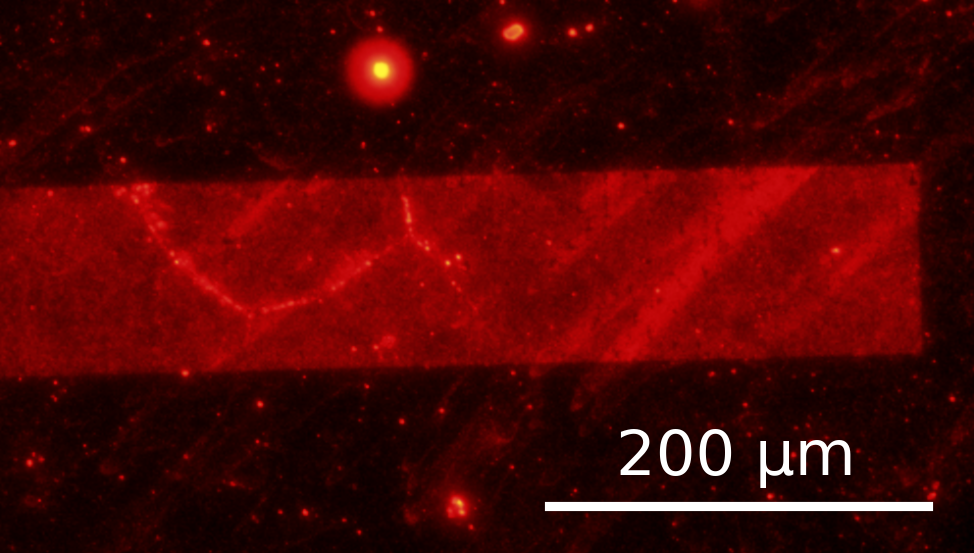
\includegraphics[width=0.5\textwidth,height=\textheight]{figures/ch2/modified_NGW8D4_1mM_rhodamineB_centralchannel3_postMsurfactantclean5min_2.4sexposure_20X_221111.png}

}

\caption{\label{fig-graphene-folds}Fluorescence image of a strip of
graphene on SiO\(_2\) surface functionalised with Rhodamine B dye.
Bright lines are visible on the left side of the graphene surface which
correspond to preferential attachment of dye along the graphene folds.}

\end{figure}

There are multiple methods for depositing graphene onto a wafer for
subsequent device fabrication, including mechanical exfoliation,
epitaxial growth and chemical vapour deposition (CVD)
\autocite{Reddy2011}. While the CVD process is relatively simple and
cheap, the initial deposition of graphene onto copper often leads to the
creation of folds (or wrinkles) of up to \(\sim\) 6 nanometers in height
across the surface of a graphene monolayer \autocite{Zhu2012}. This
occurs as a result of the rapid cooling process that takes place after
deposition, where copper thermally contracts more than graphene. Since
the graphene is pinned to the surface, this leads to slight folding of
the monolayer \autocite{Zhao2012,Zhu2012,Chhikara2013}. Transferring
graphene from the rough copper to a relatively smooth Si/SiO\(_2\) wafer
can also contribute to wrinkling \autocite{Zhao2012,Kireev2017}. These
folds help to mechanically stabilise the graphene layer, but have
significant negative effects on charge transport
\autocite{Geim2007,Chhikara2013,Zhu2012}. Folds also exhibit enhanced
reactivity due to their low radius of curvature \autocite{Zhao2012}.
This is demonstrated in Figure~\ref{fig-graphene-folds}, where the
fluorescent Rhodamine B dye preferentially bonds to folded regions,
leading to particularly dense functionalisation in these regions. This
behaviour has previously been observed for the decoration of graphene
with pentacene molecules \autocite{Chhikara2013}. Other defects
influencing surface reactivity include grain boundaries and point
defects in the crystal structure
\autocite{Zhao2012,Chhikara2013,Kireev2017}.

\hypertarget{sec-electrical-characterisation-graphene}{%
\subsection{Electrical
Characterisation}\label{sec-electrical-characterisation-graphene}}

The transfer sweep behaviour of a graphene device is ambipolar and has
no off regime under standard conditions
\autocite{Novoselov2004,Bartolomeo2011,Ohno2015}. When a gate voltage
\(V_g\) is applied to the channel of a graphene device, the Fermi energy
of the graphene is shifted and surface charge density is altered
\autocite{Novoselov2004,Heller2010,Ohno2015}. An increase in surface
charge density means an increase in carriers available for either \(p\)
or \(n\)-conduction and increased \(I_d\) \autocite{Geim2007}. The
regions of hole conduction and electron conduction are shown in
Figure~\ref{fig-graphene-characteristics} (a), alongside the
corresponding Fermi energy on the simplified graphene bandstructure
(known as a `Dirac cone'). The transconductance of the curve at \(V_g\)
= 0 V, \(g_m\) = 1 µS, is similar to the liquid-gated transconductance
of a carbon nanotube device shown earlier. As graphene lacks a bandgap,
there is a minimum possible conductance for graphene devices, which
leads to a relatively small on-off ratio
\autocite{Novoselov2004,Geim2007}. Folding may further decrease on-off
ratio due to diffusive transport of carriers along the folds
\autocite{Zhu2012}. The on-off ratio of the graphene transfer curve
shown in Figure~\ref{fig-graphene-characteristics} (a) is 5. A bandgap
can be introduced to a graphene device using a dual-gated configuration,
where both back-gate and top-gate can be swept simultaneously,
increasing the on-off ratio past 100
\autocite{Xia2010,Ahn2020,Shkodra2021}.

\begin{figure}

\begin{minipage}[t]{0.03\linewidth}

{\centering 

\raisebox{-\height}{


\includegraphics{figures/(a).png}

}

}

\end{minipage}%
%
\begin{minipage}[t]{0.01\linewidth}

{\centering 

~

}

\end{minipage}%
%
\begin{minipage}[t]{0.45\linewidth}

{\centering 

\raisebox{-\height}{

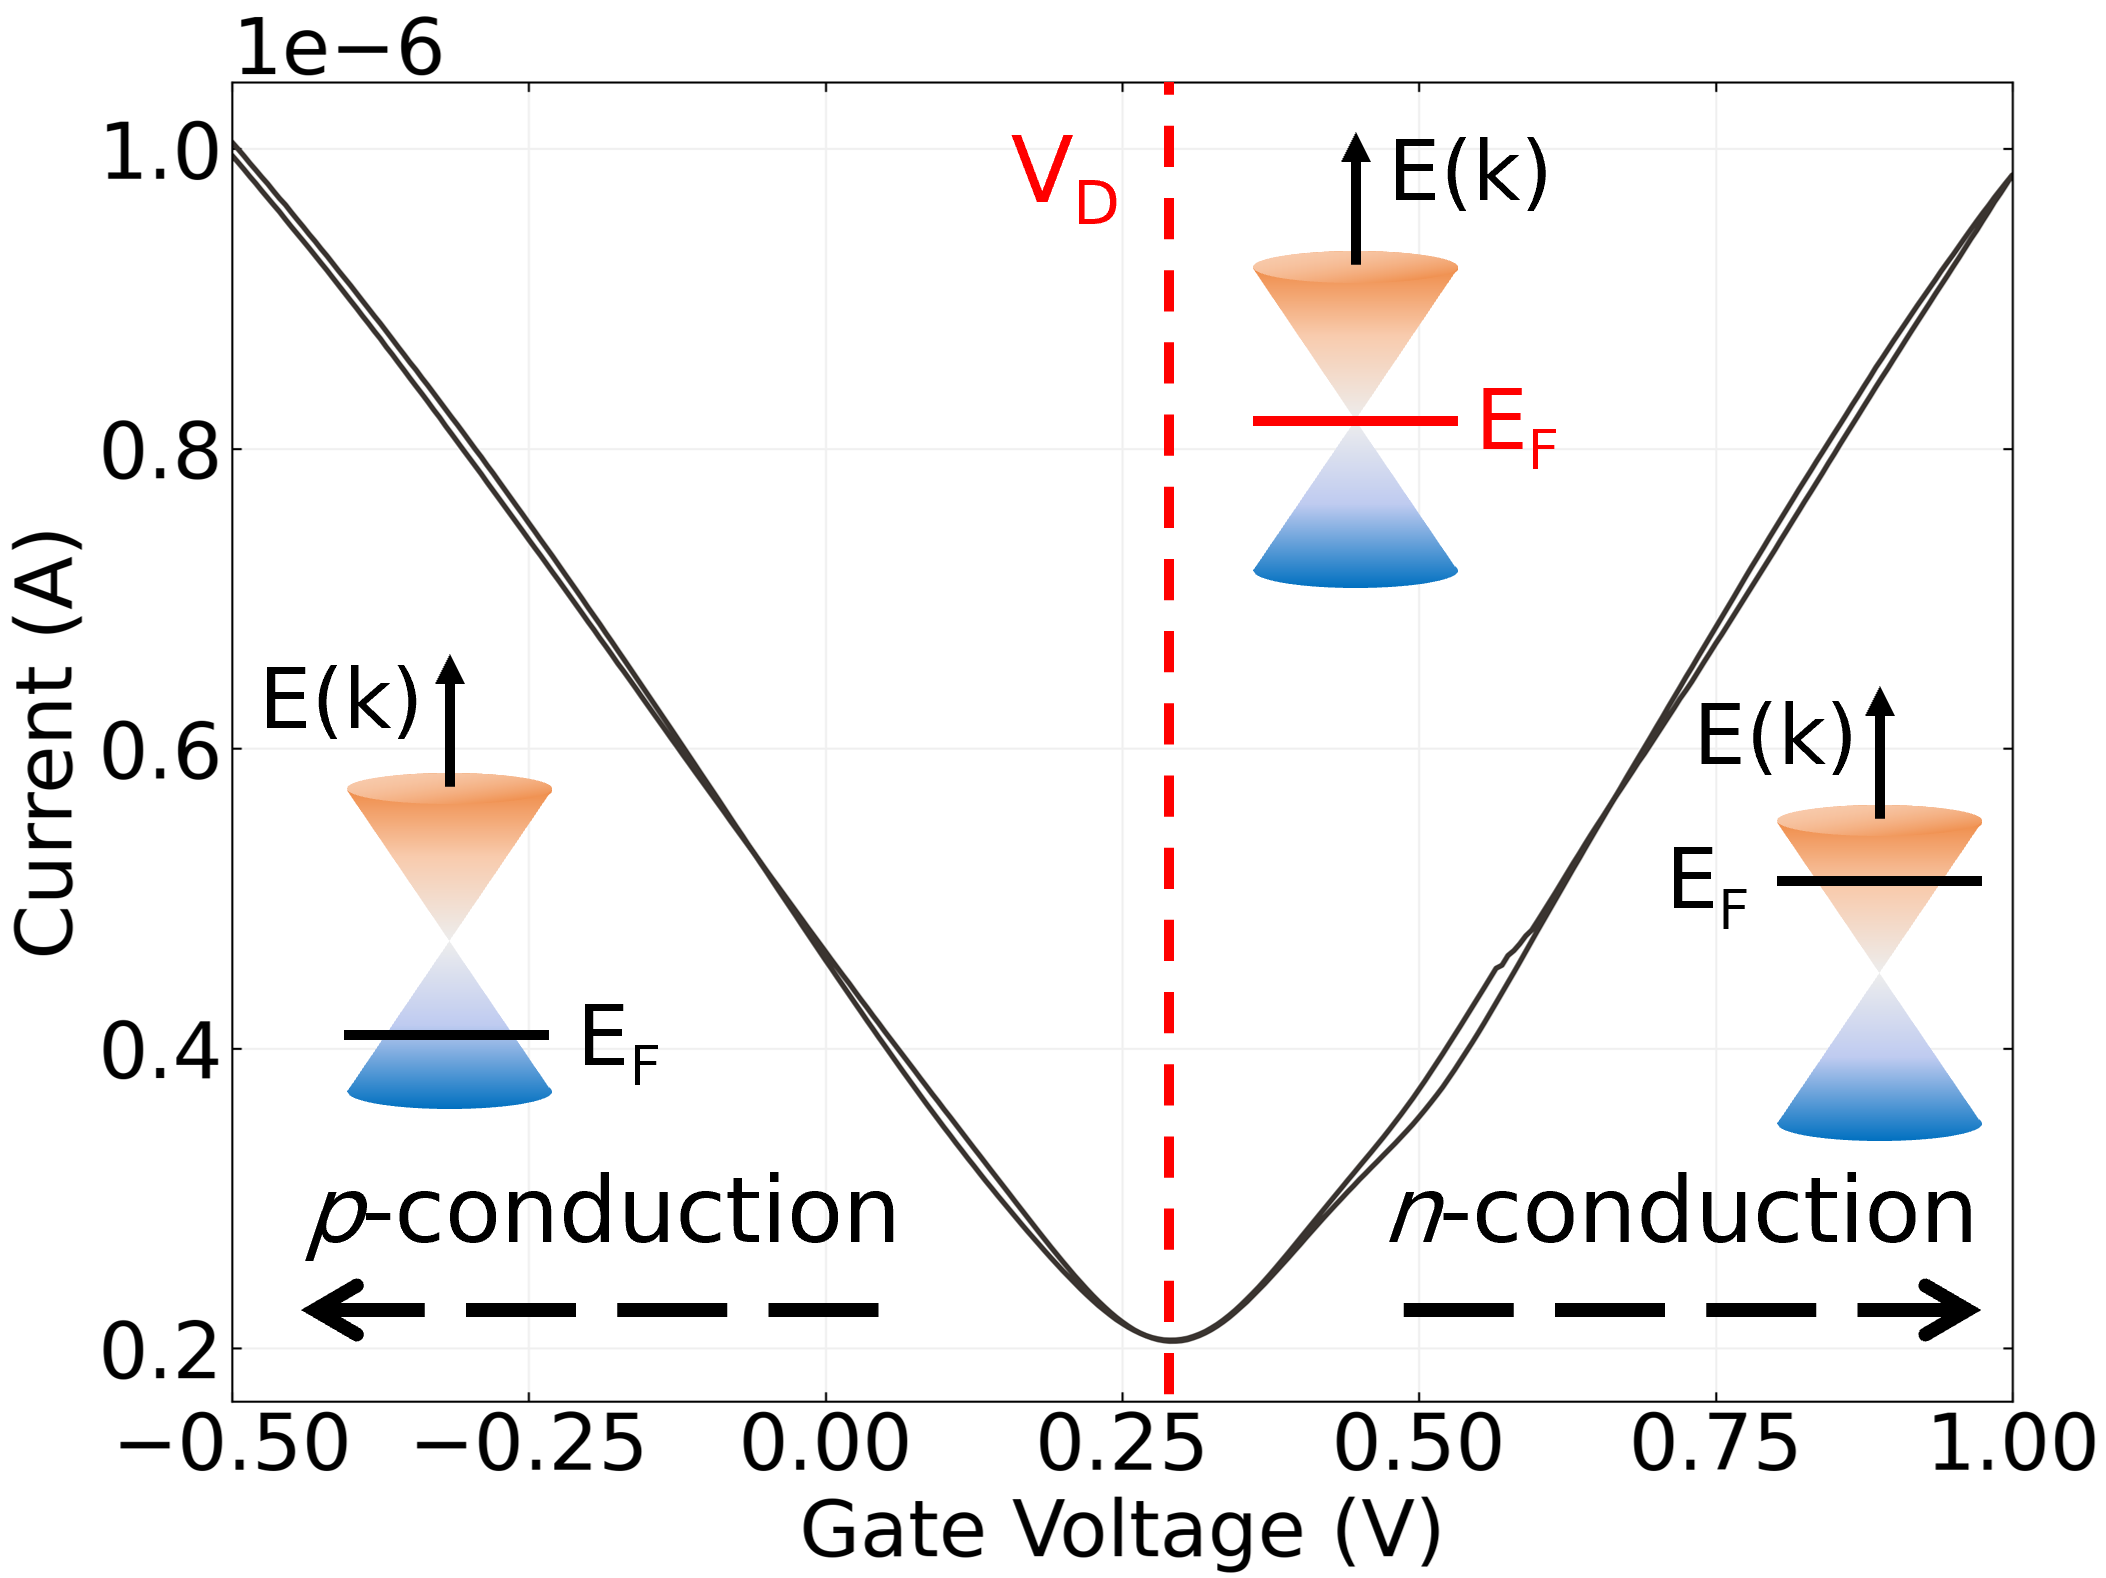
\includegraphics{figures/ch2/Graphene_transfer_1.png}

}

}

\end{minipage}%
%
\begin{minipage}[t]{0.01\linewidth}

{\centering 

~

}

\end{minipage}%
%
\begin{minipage}[t]{0.03\linewidth}

{\centering 

\raisebox{-\height}{

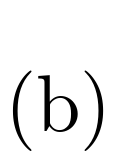
\includegraphics{figures/(b).png}

}

}

\end{minipage}%
%
\begin{minipage}[t]{0.01\linewidth}

{\centering 

~

}

\end{minipage}%
%
\begin{minipage}[t]{0.45\linewidth}

{\centering 

\raisebox{-\height}{

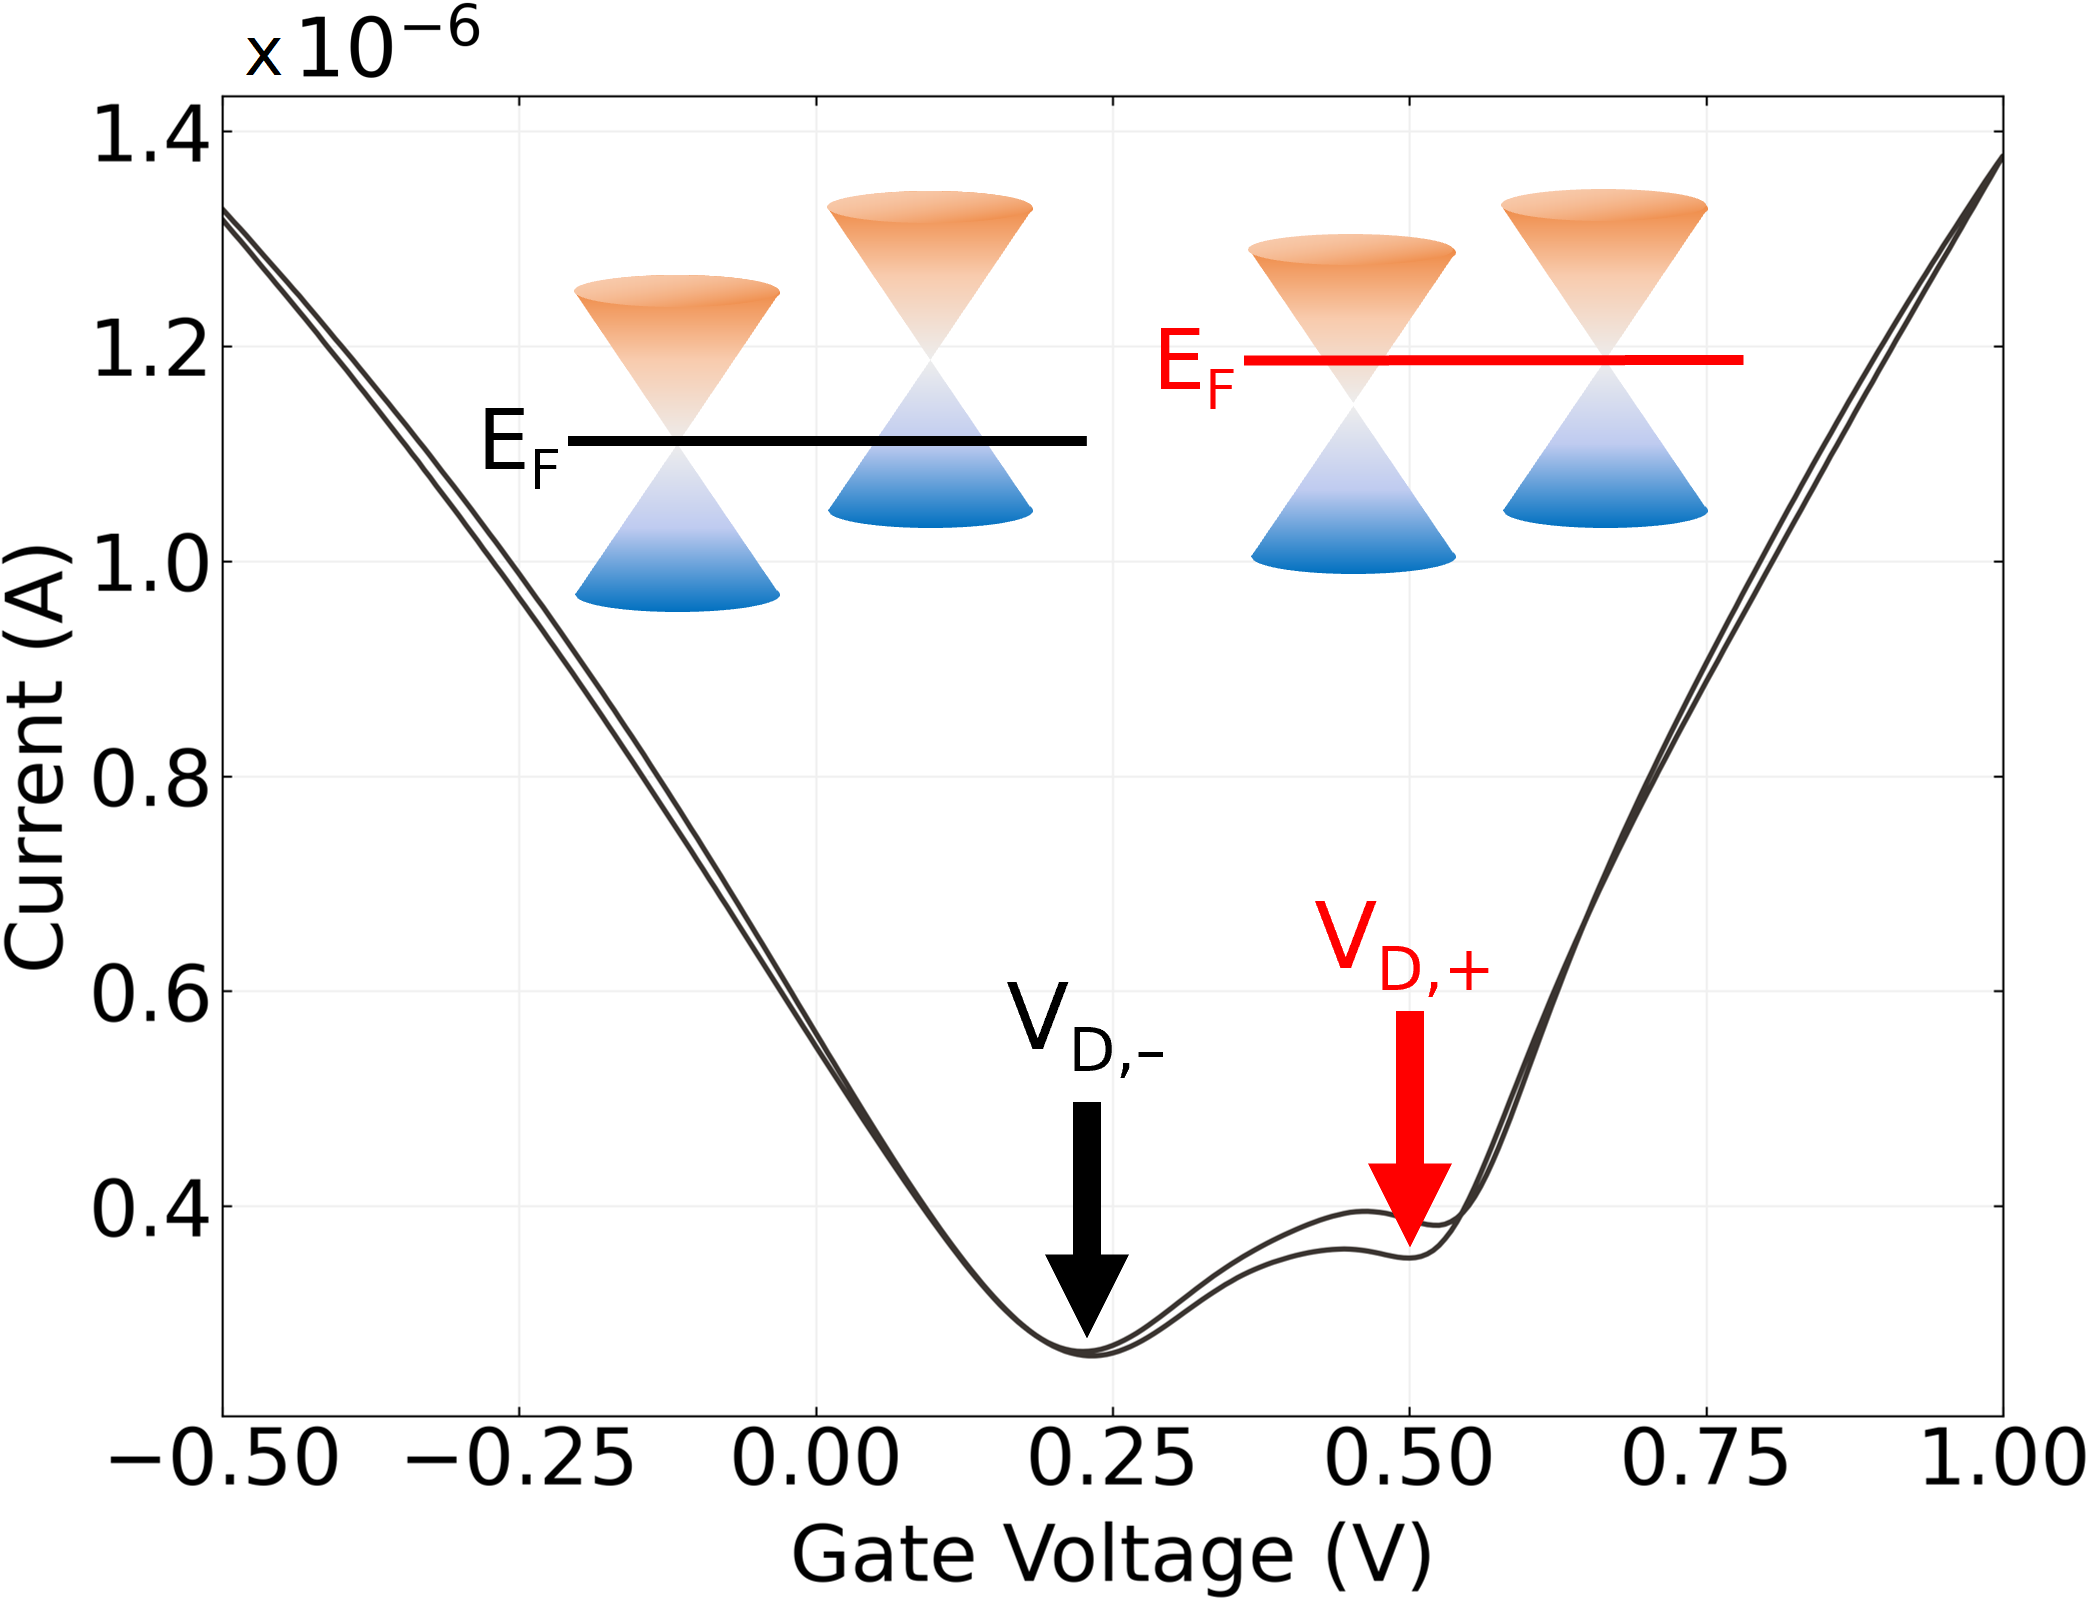
\includegraphics{figures/ch2/Graphene_transfer_2.png}

}

}

\end{minipage}%
%
\begin{minipage}[t]{0.01\linewidth}

{\centering 

~

}

\end{minipage}%

\caption{\label{fig-graphene-characteristics}Liquid-gated transfer
characteristics of two graphene field-effect transistor channels, one of
which exhibits a double-minimum feature seen in longer transistor
channels. In (a), the Dirac point voltage is indicated by a red line,
and regions of hole conduction and electron conduction are also shown.
The relative Fermi energy in each region is shown on simplified graphene
bandstructure insets (Adapted from \autocite{Geim2007,Ohno2015}). The
graphene channel in (b) has double conduction minima, which are
highlighted with red arrows. The relative Fermi energy at each minima is
also shown on bandstructure insets (Adapted from \autocite{Peng2018}).}

\end{figure}

The minimum conductance obtainable by gating in a graphene device occurs
at what is known as the charge neutrality or Dirac point, where the
population of charge carriers is at a minimum
\autocite{Novoselov2004,Bartolomeo2011,Ohno2015,Kireev2017}. At gate
voltages close to the Dirac voltage, both electrons and holes are
present, and at the Dirac point, there are equal concentrations of each
carrier present \autocite{Novoselov2004,Bartolomeo2011,Peng2018}. As
shown in Figure~\ref{fig-graphene-characteristics} (a), as the gate
voltage moves left away from the Dirac voltage and Fermi energy is
shifted into the valence band, holes begin to dominate conduction, while
as gate voltage is moved to the right of the Dirac voltage, where Fermi
energy is shifted into the conduction band, electrons dominate
\autocite{Novoselov2004,Bartolomeo2011,Feng2014,Zhang2015}. At points
far from the Dirac voltage, conductivity increases linearly
\autocite{Novoselov2004,Bartolomeo2011,Peng2018}. Typically, a monolayer
graphene channel conducts holes at zero gate voltage, which results from
the presence of \(p\)-dopants such as oxygen and water adsorbed from the
air and resist residues. By removing these dopants, the Dirac point
feature can be brought closer to the zero gate voltage position on the
transfer curve, indicating graphene is naturally a mixed-carrier
conductor
\autocite{Novoselov2004,Bartolomeo2011,Zhang2015,Kireev2017,Peng2018}.

Some graphene devices naturally exhibit a double-minimum feature in the
transfer characteristic curve, corresponding to two separate Dirac
points \autocite{Bartolomeo2011,Feng2014,Zhang2015,Kireev2017,Peng2018}.
This effect is due to doping of graphene by charge transfer from the
metal contacts. In shorter length channels, metal doping affects the
entire channel length. Band bending from channel doping near the metal
contact results in a consistent Fermi level across the channel, meaning
only a single Dirac point is present in the transfer characteristic
curve. However, for longer channels, metal doping no longer occurs
across the entire channel length \autocite{Bartolomeo2011,Peng2018}.
This discrepancy leads to a difference in Fermi level between the
metal-doped graphene and graphene in the unaffected channel region
\autocite{Bartolomeo2011,Feng2014,Peng2018,Zhang2015}. The difference in
Fermi levels results in the introduction of a second Dirac point. The
relative level of doping in the metal-doped and unaffected channel
regions determines the relative \(V_g\) position of each local minimum
on the \(I_d - V_g\) curve \autocite{Bartolomeo2011,Peng2018,Zhang2015}.

Figure~\ref{fig-graphene-characteristics} (b) shows a double-minimum
transfer characteristic with each Dirac point indicated. At large
negative \(V_g\), the Fermi energy level is far from the Dirac point
energy of both the channel and contact regions, and holes dominate
conduction. As \(V_g\) and the Fermi energy approach and then pass the
Dirac point corresponding to the left minimum \(V_{D,-}\), the available
carriers decrease to a minimum and begin to increase again in one region
\(R_1\), but continuously decrease in the other region \(R_2\). The
shape of the curve between \(V_{D,-}\) and the right local minimum
\(V_{D,+}\) then depends on the relative rate of increasing electron and
decreasing hole populations, where the graphene is \(n\)-doped in
\(R_1\) and \(p\)-doped in \(R_2\). At the local minimum on the right,
\(V_{D,+}\), the carriers in \(R_2\) now reach a minimum, while carriers
in \(R_1\) continue to increase. At voltages well beyond \(V_{D,+}\),
electrons then dominate conduction in both regions
\autocite{Bartolomeo2011,Zhang2015,Peng2018}.

\hypertarget{sensing-behaviour}{%
\subsection{Sensing Behaviour}\label{sensing-behaviour}}

The large surface-to-volume ratio of graphene makes it highly sensitive
to intermolecular interactions and therefore appropriate for use in
sensing applications \autocite{Ohno2015,Tran2016}. An analyte molecule
can be detected using a graphene channel by observing the change in
current that occurs when the presence of a charged analyte alters the
channel Fermi level \autocite{Heller2010,Ohno2015}. Sensing may be
dominated by interactions occurring at the graphene folds
\autocite{Zhao2012}. The small on-off ratio of graphene is a drawback
when used in field-effect transistor sensing applications when compared
with carbon nanotube transistors \autocite{Novoselov2004}. If a
dual-gate configuration is used, however, on-off ratio can be increased
significantly by introducing a bandgap. The presence of a bandgap means
a Schottky barrier is introduced at the graphene-electrode interface,
whose modulation can then also contribute as a potential sensing
mechanism (see Section~\ref{sec-cnt-network-details} for a discussion of
Schottky barriers) \autocite{Xia2010}.

\hypertarget{carbon-nanotube-field-effect-transistors}{%
\section{Carbon Nanotube Field-Effect
Transistors}\label{carbon-nanotube-field-effect-transistors}}

\hypertarget{sec-carbon-nanotubes}{%
\subsection{Carbon Nanotube Properties}\label{sec-carbon-nanotubes}}

\begin{figure}

{\centering 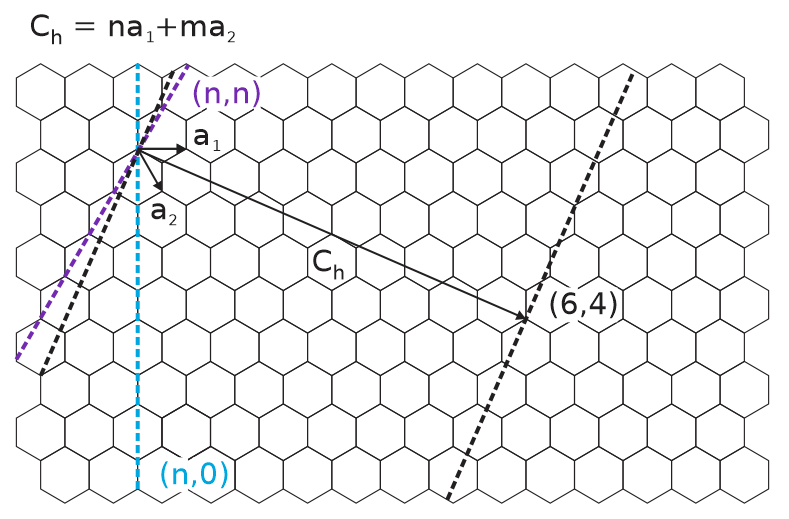
\includegraphics[width=0.6\textwidth,height=\textheight]{figures/ch2/carbon_nanotube_wrapping.png}

}

\caption{\label{fig-carbon-nanotube-wrapping}Diagram illustrating how a
graphene sheet can be rolled up at various angles to form carbon
nanotubes. The two black dotted lines represent boundaries which can be
cut across and then brought into contact to form a cylinder. The
cylinder here is referred to by the integer pair (6,4), since the chiral
vector \(C_h\), the vector perpendicular to the cut through the sheet,
is given by \(C_h = 6a_1+4a_2\). The chiral vector forms the
circumference of the rolled carbon nanotube. The left edge in the zigzag
(\(n\),0) and armchair (\(n\),\(n\)) cases are shown with a blue and
purple dotted line respectively. The location of the right edge
(diameter of the nanotube) is determined by the value chosen for \(n\).
Adapted from \autocite{Dekker1999,Lu2012}.}

\end{figure}

Since their initial identification in 1991 \autocite{Iijima1991}, a wide
range of applications for carbon nanotubes (CNTs) have been proposed,
due to their small mass, elasticity, strength, and unique electronic
properties. A single-walled carbon nanotube (SWCNT) consists of a
monolayer graphene sheet rolled up into a cylinder, while a multi-walled
carbon nanotube (MWCNT) consists of several monolayer graphene cylinders
where smaller cylinders are coaxially contained by larger cylinders
\autocite{Dekker1999,Avouris2007,Cao2009,Rouhi2010,Shkodra2021}.
Multi-walled carbon nanotubes can suffer from significant scattering at
defects leading to diffusive electron motion \autocite{Dekker1999}.
However, single-walled carbon nanotubes are relatively defect-free, and
carrier transport within nanotubes is near-ballistic at room
temperature, resulting in high carrier mobility
\autocite{Dekker1999,Avouris2007,Cao2009,Rouhi2010,Shkodra2021}. The
momentum of charge carriers in a single-walled carbon nanotube is
quantised, confining carriers to 2-dimensional slices across the
3-dimensional graphene bandstructure. If a slice contains a bandgap, the
carbon nanotube behaves as a semiconductor (s-CNT); if not, the nanotube
behaves as a metal (m-CNT) \autocite{McEuen2002}. The high
surface-to-volume ratio of small-diameter single-walled carbon nanotubes
makes them extremely sensitive and therefore particularly suitable for
sensing applications \autocite{Cao2009,Yao2021,Shkodra2021}. Like
graphene, carbon nanotubes have a large potential window, and can be
used safely in a liquid-gate environment without undergoing redox
reactions \autocite{Ohno2015}.

The chirality and diameter of a carbon nanotube determines its
electronic bandstructure and whether it has semiconducting or metallic
characteristics
\autocite{Martel1998,Dekker1999,McEuen2002,Avouris2007,Shkodra2021,Li2023}.
The chirality indices of a nanotube (\(n\),\(m\)) determines the chiral
angle at which hexagons wind around the nanotube relative to the
longitudinal axis of the nanotube. This chiral angle is the angle
between the chiral vector
\(\textbf{C}_h = n\textbf{a}_1+m\textbf{a}_2\), which maps to the
circumference of the nanotube, and the basis vector \(\textbf{a}_1\),
which is parallel to a row of hexagons. The size of the chiral angle
\(\theta\) is given by Equation~\ref{eq-chiral-angle}, and the diameter
of the resulting carbon nanotube is given by \(d=|C_h|/\pi\)
\autocite{Lu2012}.

\begin{equation}\protect\hypertarget{eq-chiral-angle}{}{
\theta = \arcsin\frac{\sqrt{3}m}{2\sqrt{n^2+nm+m^2}}, \space n > m
}\label{eq-chiral-angle}\end{equation}

When \(m=0\), \(\theta = 0°\), and the resulting carbon nanotube has a
`zigzag' structure; when \(m=n\), \(\theta = 30°\), and the carbon
nanotube has an `armchair' structure. When \(\theta\) is between
\(0°-30°\), the structure is referred to as `chiral'
\autocite{Dekker1999,Lu2012}. When \(n-m=3z\), where \(z\) is an
integer, the resulting carbon nanotube is metallic \(-\) for example, if
\(n=5\) and \(m=5\), \(z=0\), therefore the tube is metallic. All other
nanotubes are semiconducting, including the (6,4) chiral nanotube
described in Figure~\ref{fig-carbon-nanotube-wrapping}. Out of the
chiral arrangements available, two-thirds of the possible structures are
semiconducting while one-third is metallic \autocite{Dekker1999}.

\hypertarget{sec-cnt-network-details}{%
\subsection{Carbon Nanotube Network
Transistors}\label{sec-cnt-network-details}}

The first carbon nanotube transistors were created in 1998, and used a
single carbon nanotube as the device channel
\autocite{Martel1998,Tans1998,Kauffman2008}. Over the following decade,
there was a general move away from the use of a single tube as the
transistor channel towards that of a large-scale network of carbon
nanotubes. In these networks, the individual electrical properties of
the CNTs are averaged out across the network, reducing device-to-device
variation. Furthermore, the large area of coverage ensures high channel
mobility. The network morphology is therefore generally preferred in
sensing applications \autocite{Hu2004,Cao2009,Murugathas2019,Li2023}.
The carbon nanotube network used for the channel can either be
directionally-aligned or randomly deposited
\autocite{Cao2009,Shkodra2021}; in this thesis, randomly deposited
networks were fabricated using facile solution-deposition methods
\autocite{Zheng2017,Cassie2023}. Important attributes of a carbon
nanotube film include the density of the network (number of nanotubes
per unit area), the ratio of metallic to semiconducting nanotubes
present, and the distribution of nanotube diameters present
\autocite{Cao2009,Shkodra2021}. The strong van der Waals forces between
carbon nanotubes lead to them bundling together within a network. These
bundles may contain many nanotubes of different size and chirality
\autocite{Fuhrer2000,Hu2004,Cao2009,Murugathas2019}.

The band bending which occurs at the interface between the metal
electrodes of the device and the semiconducting carbon nanotubes is
primarily responsible for carbon nanotube field-effect transistor
switching behaviour \autocite{Avouris2007,Bargaoui2018}. The Fermi level
difference between materials leads to free electrons flowing across each
interface until the Fermi levels equilibrate and a electric dipole layer
forms. The net electric field created at each interface creates a space
charge region in the channel, resulting in a potential step known as a
``Schottky barrier''. The net electric field also results in curvature
of the bandstructure at the metal-semiconductor interface, which is why
this process is referred to as ``band bending'' \autocite{Zhang2012}.
Current primarily flows through the semiconductor channel by
quantum-mechanically tunnelling through the Schottky barriers present at
each electrode. The width of the Schottky barriers can be modulated by
changing the gate voltage of the device, which can increase or decrease
current flow across the channel depending on the magnitude and polarity
of the gate voltage \autocite{Avouris2007,Bargaoui2018}. As CNT FETs are
ambipolar, it is possible for both holes and electrons to flow across
the channel; highly negative gate voltages lead to hole conduction while
positive voltages lead to electron conduction \autocite{Avouris2007}.

\begin{figure}

\begin{minipage}[t]{0.03\linewidth}

{\centering 

\raisebox{-\height}{


\includegraphics{figures/(a).png}

}

}

\end{minipage}%
%
\begin{minipage}[t]{0.01\linewidth}

{\centering 

~

}

\end{minipage}%
%
\begin{minipage}[t]{0.45\linewidth}

{\centering 

\raisebox{-\height}{

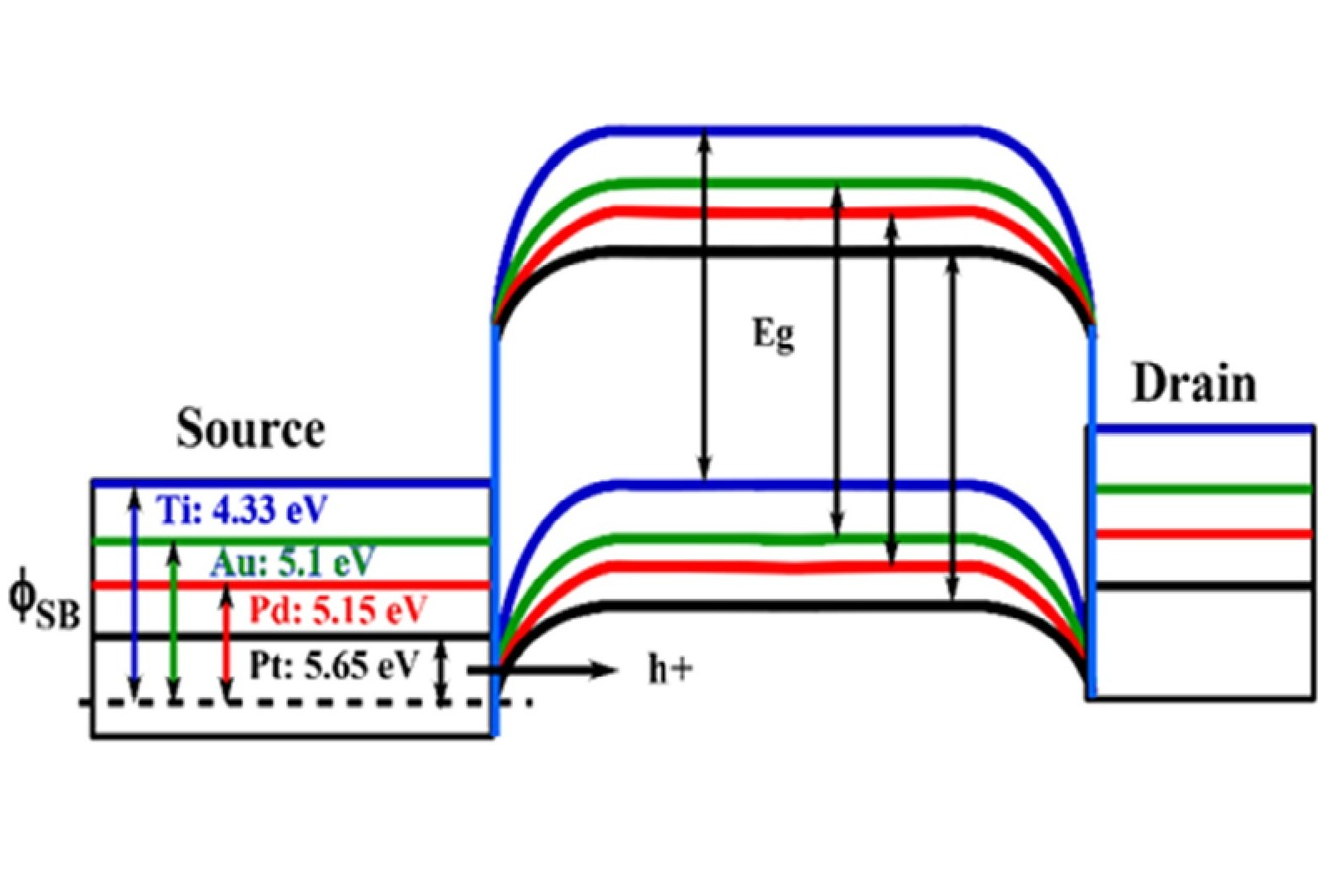
\includegraphics{figures/ch2/band-bending.png}

}

}

\end{minipage}%
%
\begin{minipage}[t]{0.01\linewidth}

{\centering 

~

}

\end{minipage}%
%
\begin{minipage}[t]{0.03\linewidth}

{\centering 

\raisebox{-\height}{

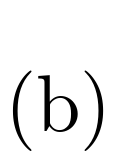
\includegraphics{figures/(b).png}

}

}

\end{minipage}%
%
\begin{minipage}[t]{0.01\linewidth}

{\centering 

~

}

\end{minipage}%
%
\begin{minipage}[t]{0.45\linewidth}

{\centering 

\raisebox{-\height}{

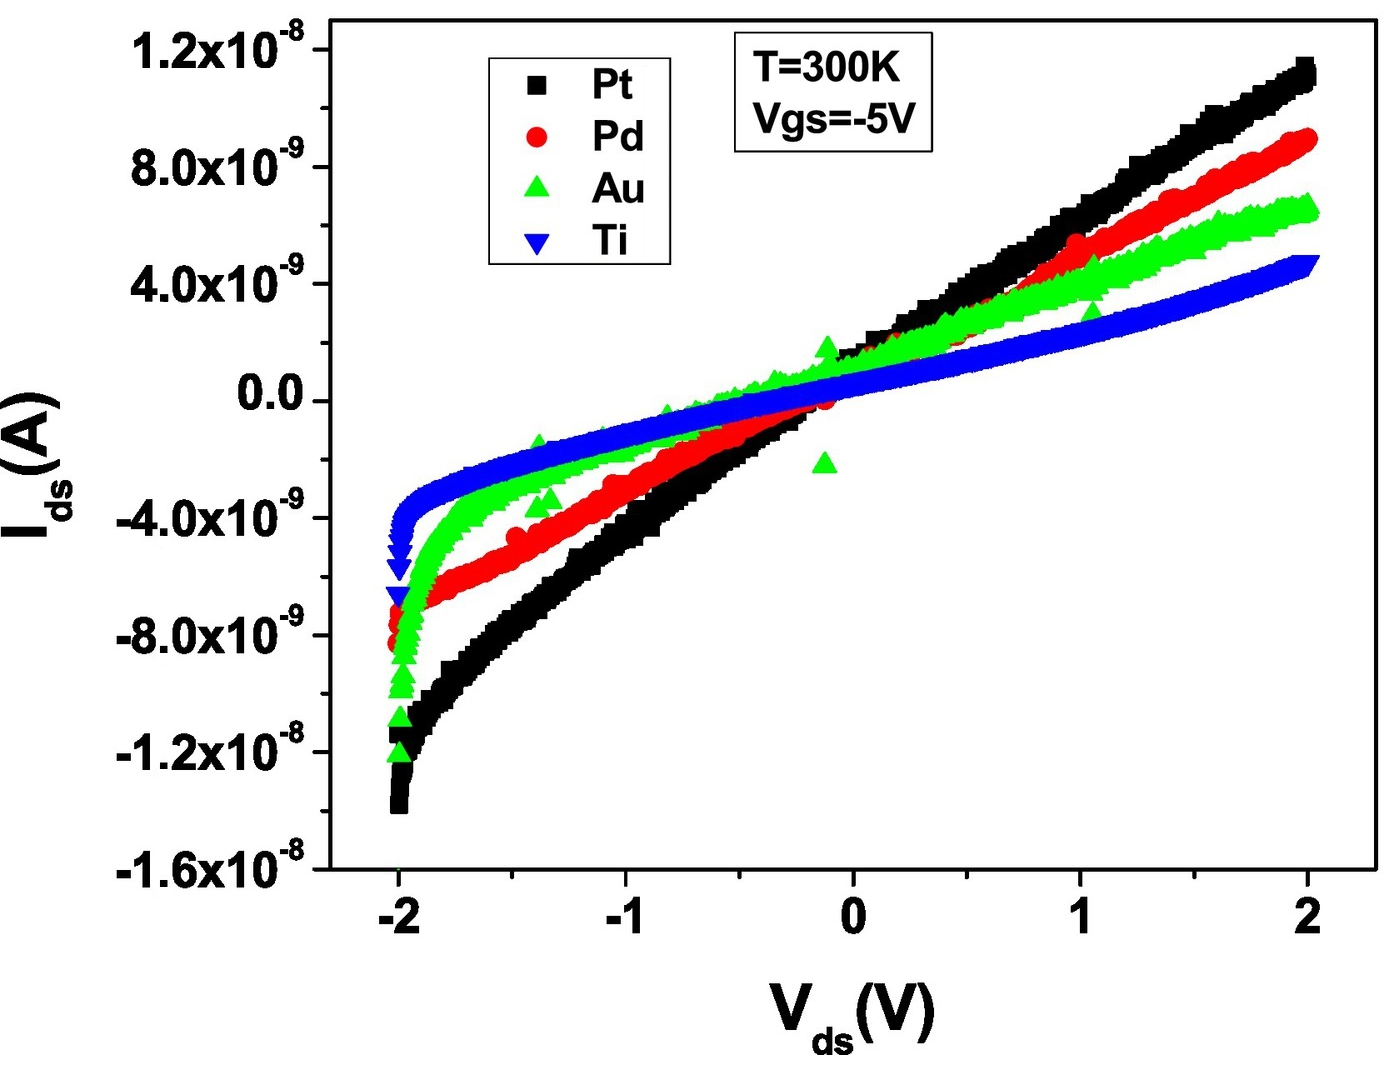
\includegraphics{figures/ch2/band-bending-current.png}

}

}

\end{minipage}%
%
\begin{minipage}[t]{0.01\linewidth}

{\centering 

~

}

\end{minipage}%

\caption{\label{fig-band-bending}The band bending which occurs at the
metal-network interface is shown in (a) for platinum, palladium, gold
and titanium electrodes, where \(\phi_{SB}\) is Schottky barrier height
and \(E_g\) is bandgap size. The output characteristic curves of devices
with these electrodes are shown in (b), where the devices are gated
fully on at \(V_g = -5\) V. Both figures reproduced with permission from
\autocite{Bargaoui2018}.}

\end{figure}

The relative height of the Schottky barriers present at the electrical
contacts influences the magnitude of on-current obtainable by a device.
An important factor in determining the Schottky barrier height of a
device is the type of metal used for the contact, with the relationship
between the type of metal used and resulting device on-current shown in
Figure~\ref{fig-band-bending}. Titanium has a relatively low work
function of 4.3 eV, leading to larger Schottky barriers at the
electrodes and relatively low device on-current, while platinum has a
relatively high work function of 5.7 eV, leading to smaller Schottky
barriers and relatively high device on-current \autocite{Bargaoui2018}.
The Schottky barrier height also influences the size of hole on-current
relative to electron on-current. A high work function metal like
palladium bends the valence band of the semiconductor towards the Fermi
level of the metal, creating a low barrier for holes but a high barrier
for electrons, leading to a much higher hole on-current as compared to
electron on-current. A low work function metal like aluminium, on the
other hand, has a relatively low work function, giving rise to a larger
on-current for electrons and smaller on-current for holes
\autocite{Chen2005,Avouris2007,Bargaoui2018}.

\begin{figure}

\begin{minipage}[t]{0.03\linewidth}

{\centering 

\raisebox{-\height}{


\includegraphics{figures/(a).png}

}

}

\end{minipage}%
%
\begin{minipage}[t]{0.01\linewidth}

{\centering 

~

}

\end{minipage}%
%
\begin{minipage}[t]{0.50\linewidth}

{\centering 

\raisebox{-\height}{

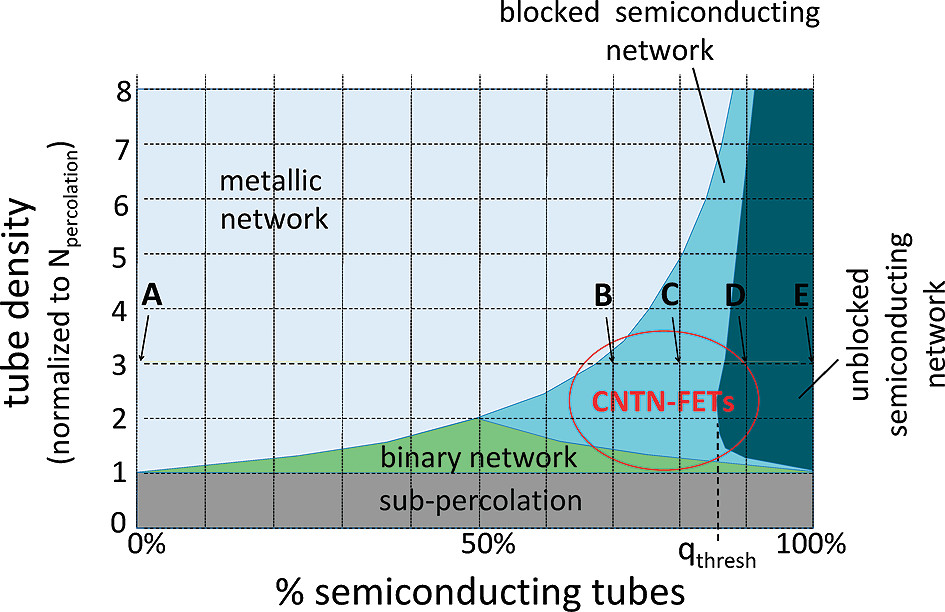
\includegraphics{figures/ch2/semiconducting-proportion-density.png}

}

}

\end{minipage}%
%
\begin{minipage}[t]{0.01\linewidth}

{\centering 

~

}

\end{minipage}%
%
\begin{minipage}[t]{0.03\linewidth}

{\centering 

\raisebox{-\height}{

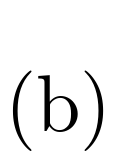
\includegraphics{figures/(b).png}

}

}

\end{minipage}%
%
\begin{minipage}[t]{0.01\linewidth}

{\centering 

~

}

\end{minipage}%
%
\begin{minipage}[t]{0.40\linewidth}

{\centering 

\raisebox{-\height}{

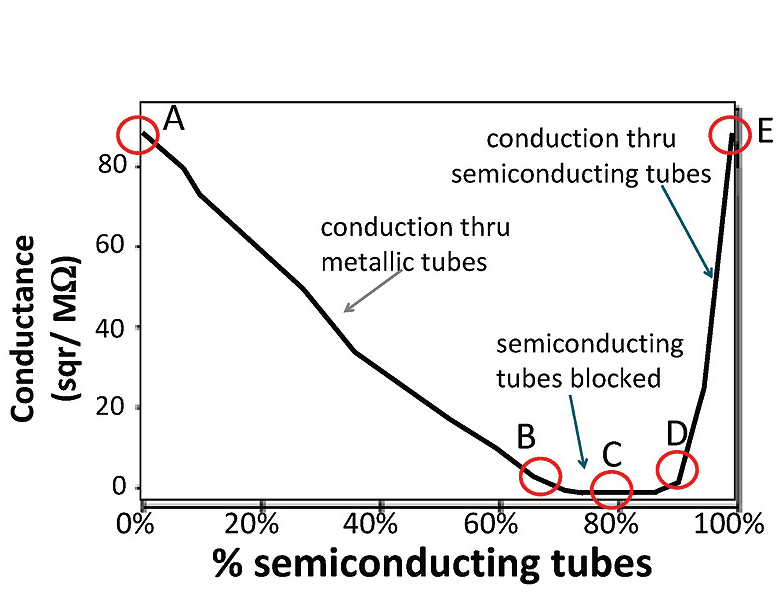
\includegraphics{figures/ch2/semiconducting-proportion.png}

}

}

\end{minipage}%
%
\begin{minipage}[t]{0.01\linewidth}

{\centering 

~

}

\end{minipage}%

\caption{\label{fig-m-s-junctions}The phase diagram in (a) shows the
relationship between the proportion of semiconducting tubes present, the
network density relative to the percolation threshold, and the general
electronic behaviour of the resulting carbon nanotube network. The
relationship between network conductance and proportion of
semiconducting tubes present is shown in (b), in the specific case where
density was roughly 3 times the percolation threshold (in the case where
all tubes were either metallic or semiconducting). Specific morphologies
A, B, C, D and E are shown on both figures. Both figures have been
reproduced with permission from \autocite{Topinka2009}.}

\end{figure}

The behaviour of carbon nanotube network transistors is also influenced
by a variety of potential barriers existing at junctions between carbon
nanotubes. A prominent example is the Schottky barriers existing at
junctions between metallic and semiconducting nanotubes (m-s junctions)
\autocite{Fuhrer2000,Topinka2009,Murugathas2019}. These potential
barriers lead to increased resistance at m-s junctions relative to other
points in the network \autocite{Fuhrer2000,Jang2015}. When the channel
length is much larger than that of individual nanotubes, channel current
must pass through junctions placed along percolating pathways. When a
network with density well above the percolation threshold\footnote{If
  only one electrical pathway exists across a sparse network, the
  network density is at the `percolation threshold'. If network density
  is below the percolation threshold, the channel cannot conduct
  \autocite{Hu2004,Topinka2009,Jang2015}.} contains a low proportion of
semiconducting nanotubes, labelled A in Figure~\ref{fig-m-s-junctions},
percolating pathways which only contain metallic nanotubes can exist. A
device with this film will be highly conductive but is practically
unaffected by gating \autocite{Fuhrer2000,Topinka2009}. Fixing the
density but increasing the proportion of s-CNTs gives the morphology C
shown in Figure~\ref{fig-m-s-junctions} (a). As m-s junctions become
more prevalent, the introduced Schottky barriers cause a dramatic drop
in conductance, as shown in Figure~\ref{fig-m-s-junctions} (b). As the
proportion of s-CNTs approaches 100\% (E in
Figure~\ref{fig-m-s-junctions}), semiconducting pathways with no
metallic junctions emerge, and conductance sharply increases once more
\autocite{Topinka2009}.

\hypertarget{sec-electrical-characterisation-CNT}{%
\subsection{Electrical
Characterisation}\label{sec-electrical-characterisation-CNT}}

Like graphene transistors, mixed-chirality carbon nanotube transistors
are naturally ambipolar: they can conduct both electrons and holes. An
applied gate voltage \(V_g\) alters the Fermi energy of the
semiconducting nanotubes, modulating the width of the Schottky barriers
present, and therefore changing the amount and type of charge flowing
through the channel \autocite{Nakanishi2002,Kauffman2008,Heller2008}.
Diameter and separation of nanotubes both influence the gate capacitance
of carbon nanotube networks alongside geometric capacitance \(C_{G}\)
and quantum capacitance \(C_{Q}\) \autocite{Rouhi2011a}. \(I_d\) mainly
consists of holes at highly negative gate voltages, and mainly consists
of electrons at highly positive voltages. At intermediary voltages, both
electrons and holes flow \autocite{Avouris2007,Yao2021}. Transistor
behaviour can be made unipolar through doping the semiconducting carbon
nanotubes or by choosing an electrode metal with a particularly high
work function, increasing the Schottky barrier for one type of charge
\autocite{Avouris2007,Kauffman2008,Cao2009,Yao2021}. For example, the
use of gold electrodes promotes \(p\)-type behaviour over \(n\)-type
behaviour due to the work function of the metal; ambient adsorption of
oxygen will weakly dope the semiconducting carbon nanotubes and likewise
promote \(p\)-type behaviour
\autocite{McEuen2002,Kauffman2008,Cao2009,Shkodra2021}.

A variety of parameters can be extracted which reflect the morphology of
the carbon nanotube network. Partial alignment of a random-network
carbon nanotube network maximises the transconductance of a device, as
this creates more semiconducting pathways, increasing current while
preserving the presence of gateable junctions within the network
\autocite{Cao2009,Rouhi2010,Rouhi2011a,Jang2015,Li2023}. The on-off
ratio of a carbon nanotube device is largely decided by the ratio of
s-CNTs to m-CNTs. The relative proportion of metallic carbon nanotubes
in the network determines the relative size of \(I_{off}\). Therefore,
unlike a graphene device, the off current can be tuned by adjusting the
relative proportion of metallic nanotubes present
\autocite{Hu2004,Kauffman2008,Cao2009,Rouhi2011a}. In a liquid-gated
environment, the gate leakage current of a sparse carbon nanotube
transistor can approach \(I_d\), leading to significant device noise. A
dense network or a graphene device can therefore give enhanced
signal-to-noise ratio during sensing \autocite{Ohno2015}. Noyce \emph{et
al.} found that fully-on back-gated carbon nanotube devices typically
exhibit a \(\sim\) 3 hour period of steep signal drift, followed by
steady-state current flow. This settling behaviour was both reversible
and highly characteristic of a particular channel, and could be modelled
using a sum of three exponentials \autocite{Noyce2019}.

\begin{figure}

\begin{minipage}[t]{0.03\linewidth}

{\centering 

\raisebox{-\height}{


\includegraphics{figures/(a).png}

}

}

\end{minipage}%
%
\begin{minipage}[t]{0.01\linewidth}

{\centering 

~

}

\end{minipage}%
%
\begin{minipage}[t]{0.45\linewidth}

{\centering 

\raisebox{-\height}{

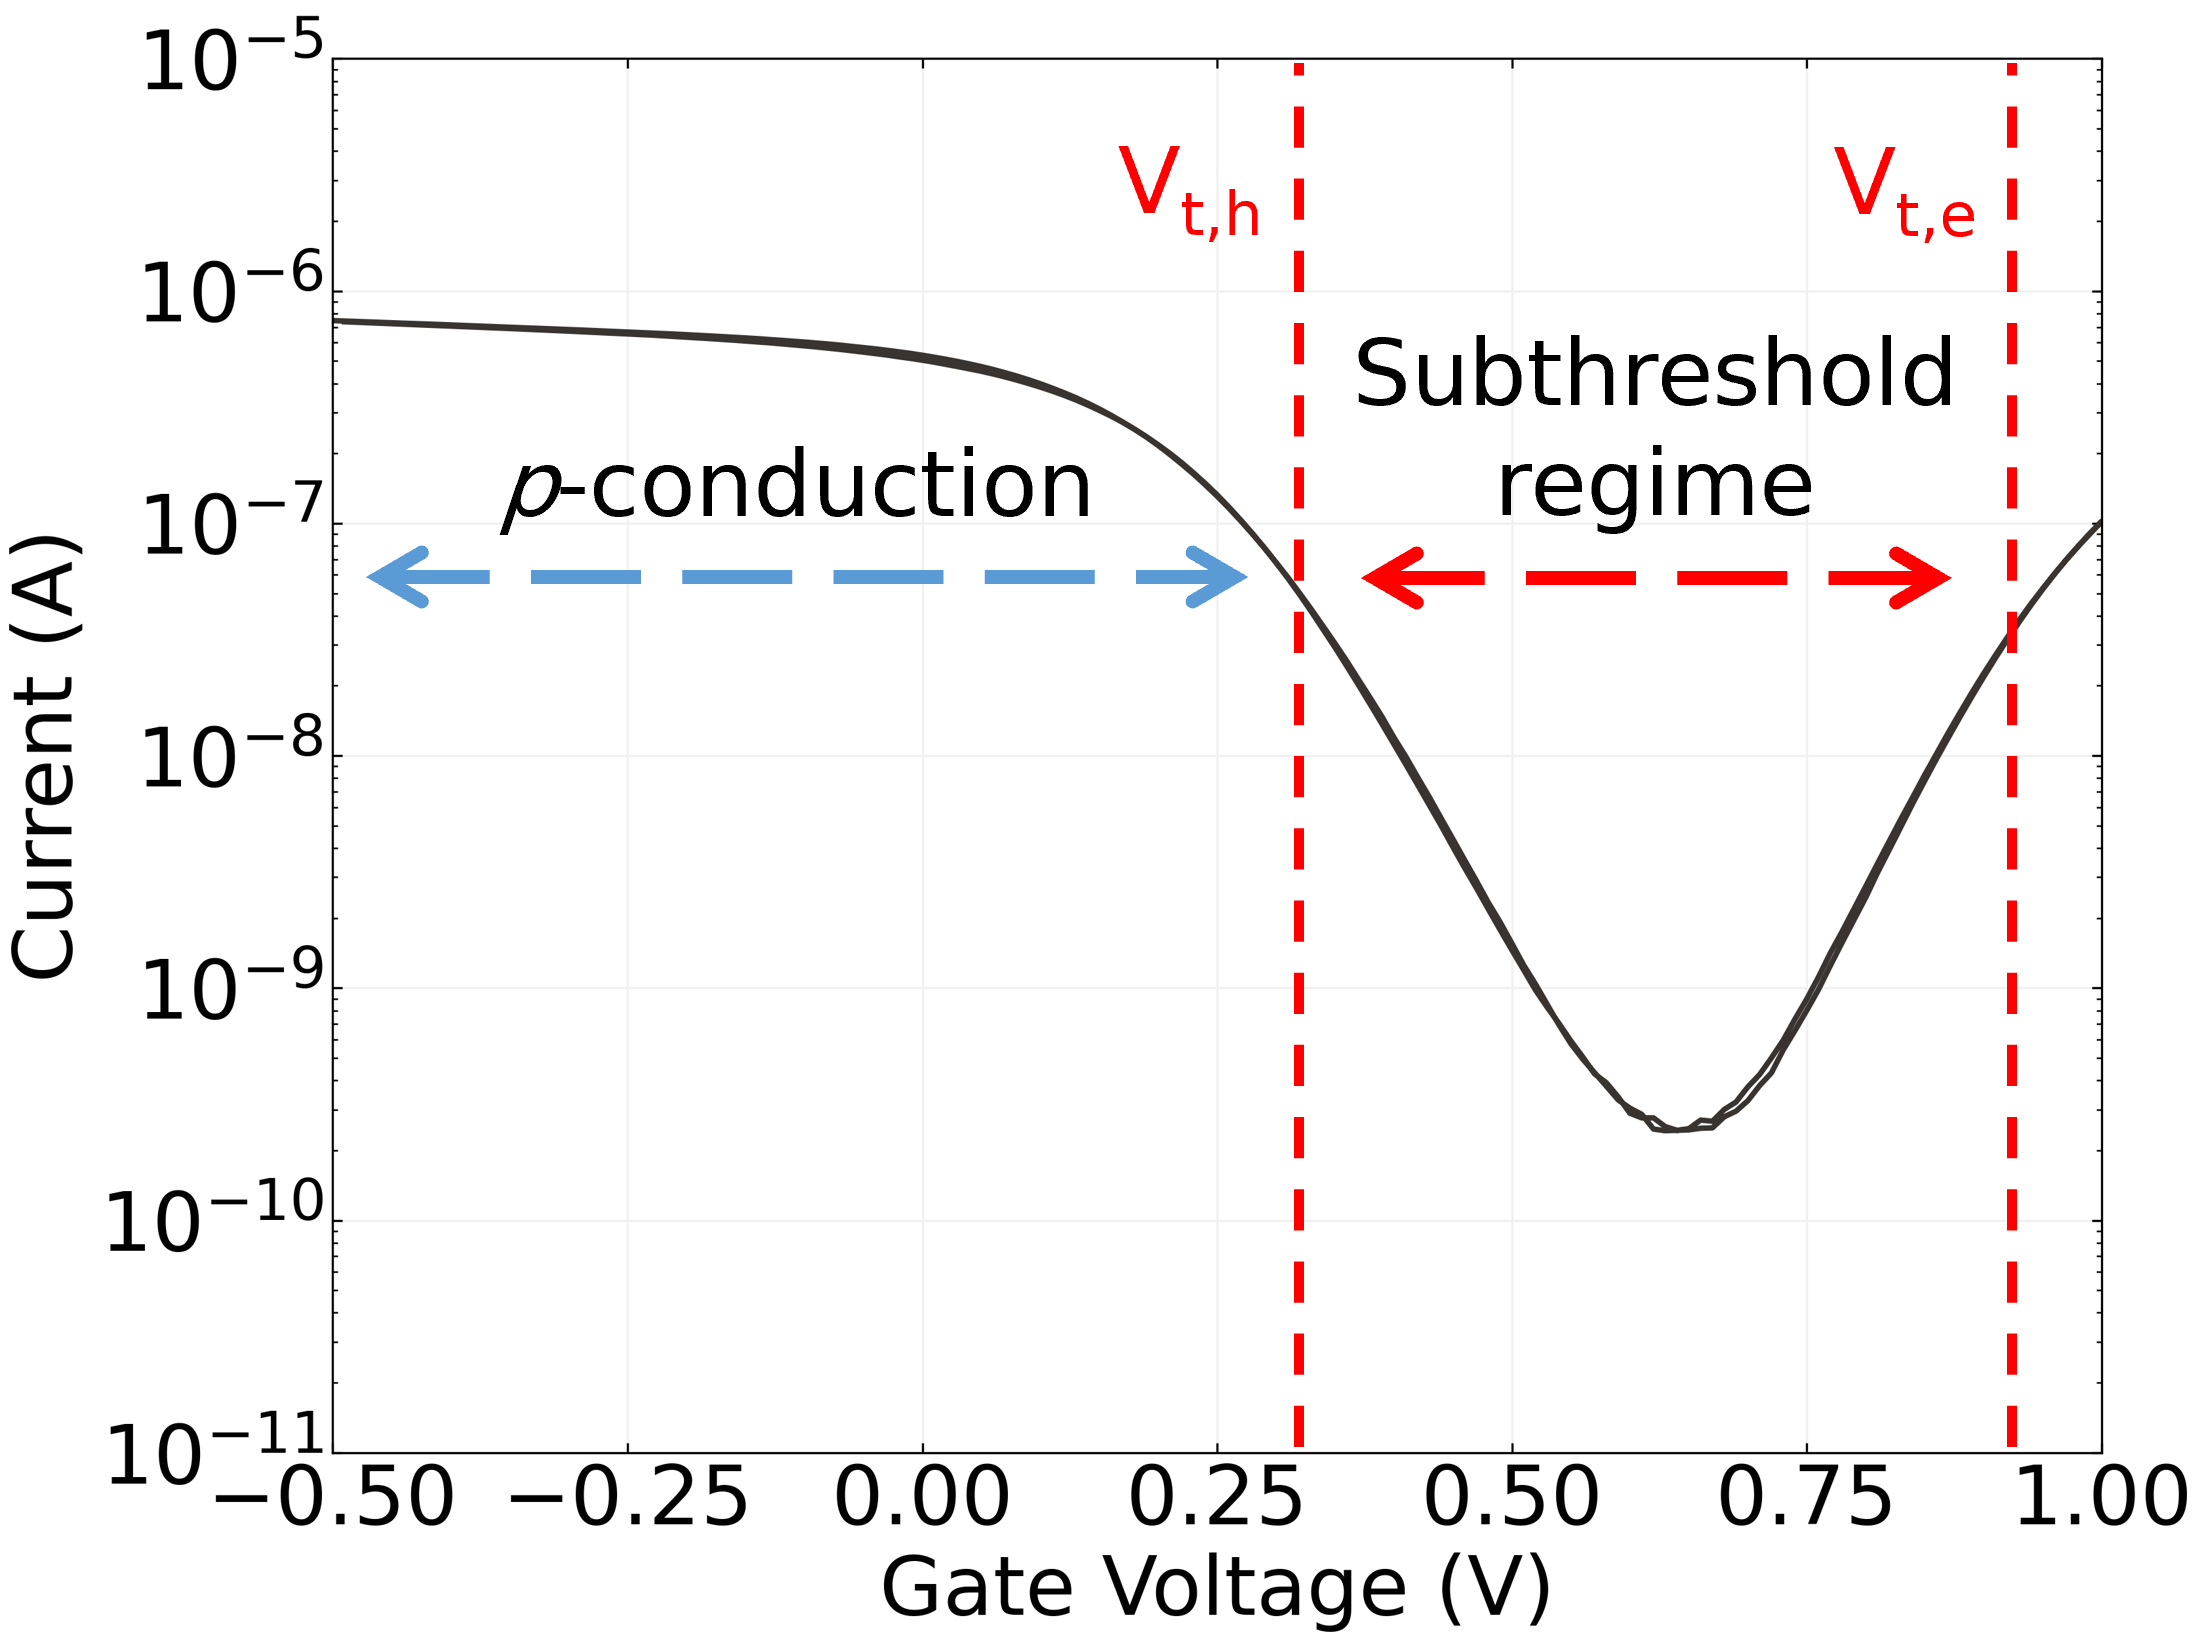
\includegraphics{figures/ch2/CNT_transfer_1.png}

}

}

\end{minipage}%
%
\begin{minipage}[t]{0.01\linewidth}

{\centering 

~

}

\end{minipage}%
%
\begin{minipage}[t]{0.03\linewidth}

{\centering 

\raisebox{-\height}{

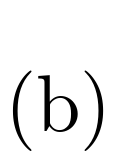
\includegraphics{figures/(b).png}

}

}

\end{minipage}%
%
\begin{minipage}[t]{0.01\linewidth}

{\centering 

~

}

\end{minipage}%
%
\begin{minipage}[t]{0.45\linewidth}

{\centering 

\raisebox{-\height}{

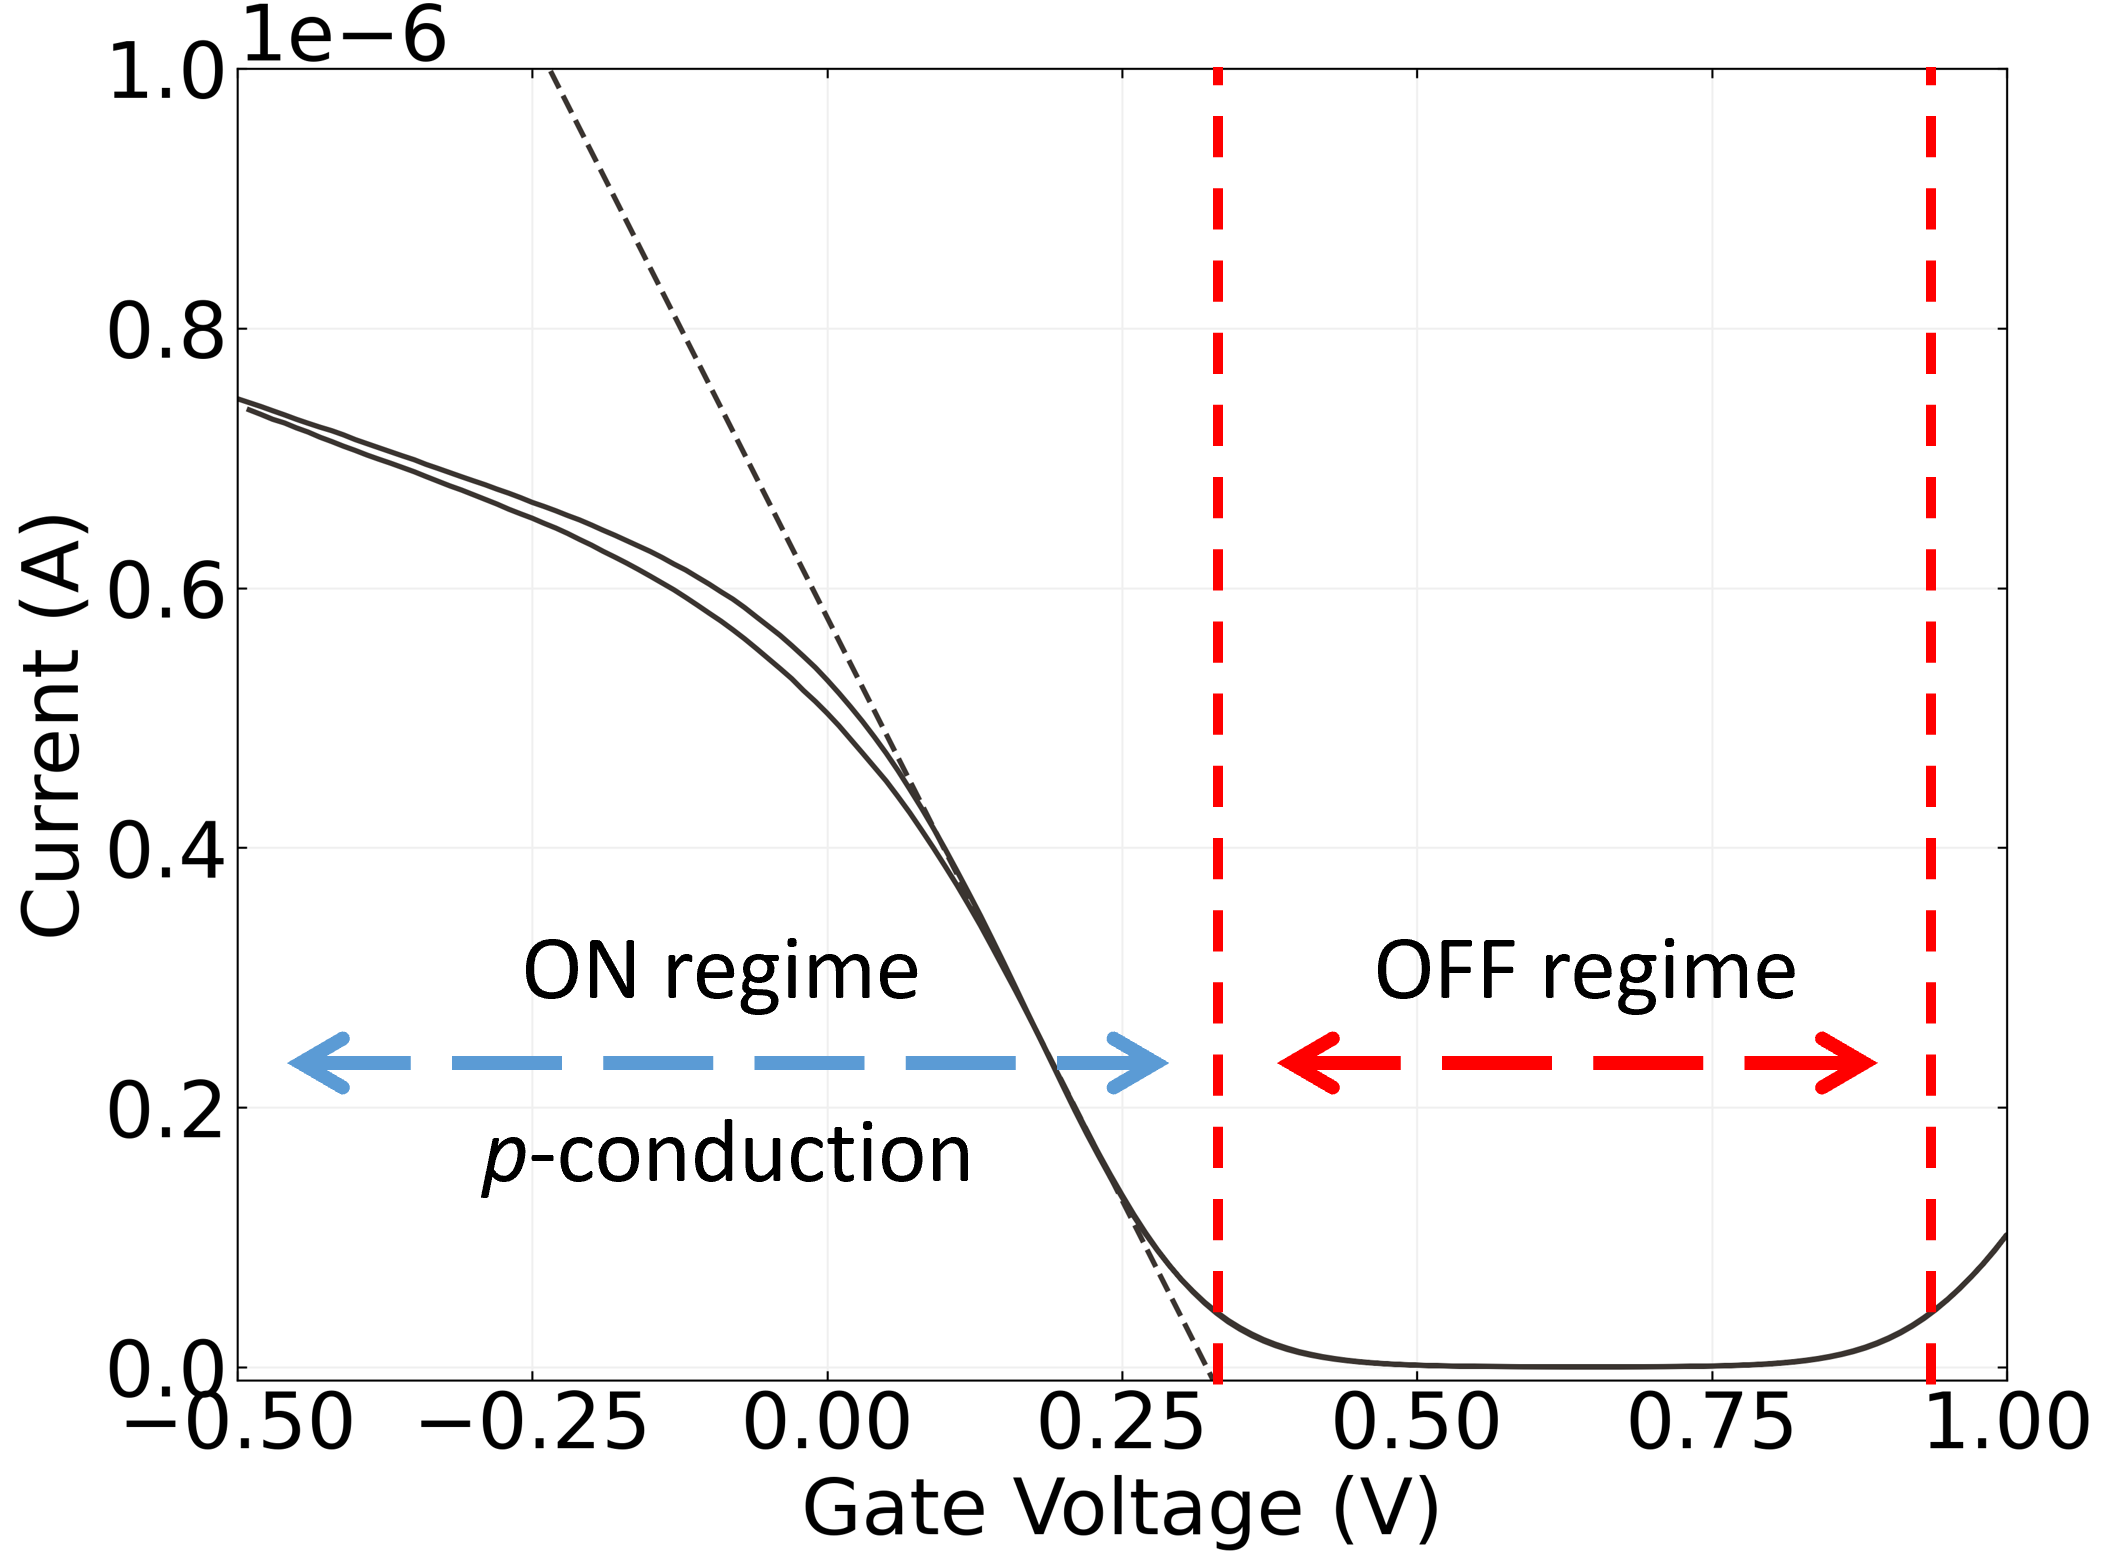
\includegraphics{figures/ch2/CNT_transfer_2.png}

}

}

\end{minipage}%
%
\begin{minipage}[t]{0.01\linewidth}

{\centering 

~

}

\end{minipage}%

\caption{\label{fig-CNT-characteristics}Liquid-gated transfer
characteristics of a single carbon nanotube network field-effect
transistor channel, using a logarithmic scale in (a) and using a linear
scale in (b) to emphasise different features of the same dataset. The
subthreshold slope is shown with a black dotted line, while the
threshold voltages are shown with red dotted lines. The ON and OFF
regimes are also indicated on both figures. \(V_{ds}\) = 100 mV was
placed across the channel.}

\end{figure}

The threshold voltage \(V_t\) of a unipolar transistor is equal to the
gate voltage required to prevent the flow of charge carriers across the
channel, often referred to as turning the device off
\autocite{Petti2016,Shkodra2021}. In ambipolar devices, two separate
threshold voltages exist for each type of charge carrier, \(V_{t,h}\)
and \(V_{t,e}\), which are shown in Figure~\ref{fig-CNT-characteristics}
on both a linear (a) and logarithmic (b) scale. In the region between
these gate voltages, known as the subthreshold regime, both holes and
electrons flow through the channel
\autocite{Avouris2007,Reiner-Rozman2015}. If percolating pathways
consisting entirely of m-CNTs are present, \(I_{off}\) flows through
these pathways, as conduction through metallic nanotubes is largely
unaffected by changes in \(V_g\) \autocite{Fuhrer2000,Topinka2009}. If
there are no unblocked m-CNT pathways, \(I_{off}\) is entirely due to
Schottky barrier tunnelling \autocite{Avouris2007}. \(V_t\) can be
estimated by extrapolating the trendline of the linear region of the
transfer characteristics to the \(V_g\) axis. The intercept is
approximately equal to the threshold voltage when \(V_{ds}\) is close to
zero, as shown in Figure~\ref{fig-CNT-characteristics} (b)
\autocite{Sze2006,Petti2016,Li2023}. This is only a rough estimate of
the actual device \(V_t\), but is sufficient when comparing the gating
behaviour of different devices \autocite{Li2023}.

\begin{figure}

{\centering 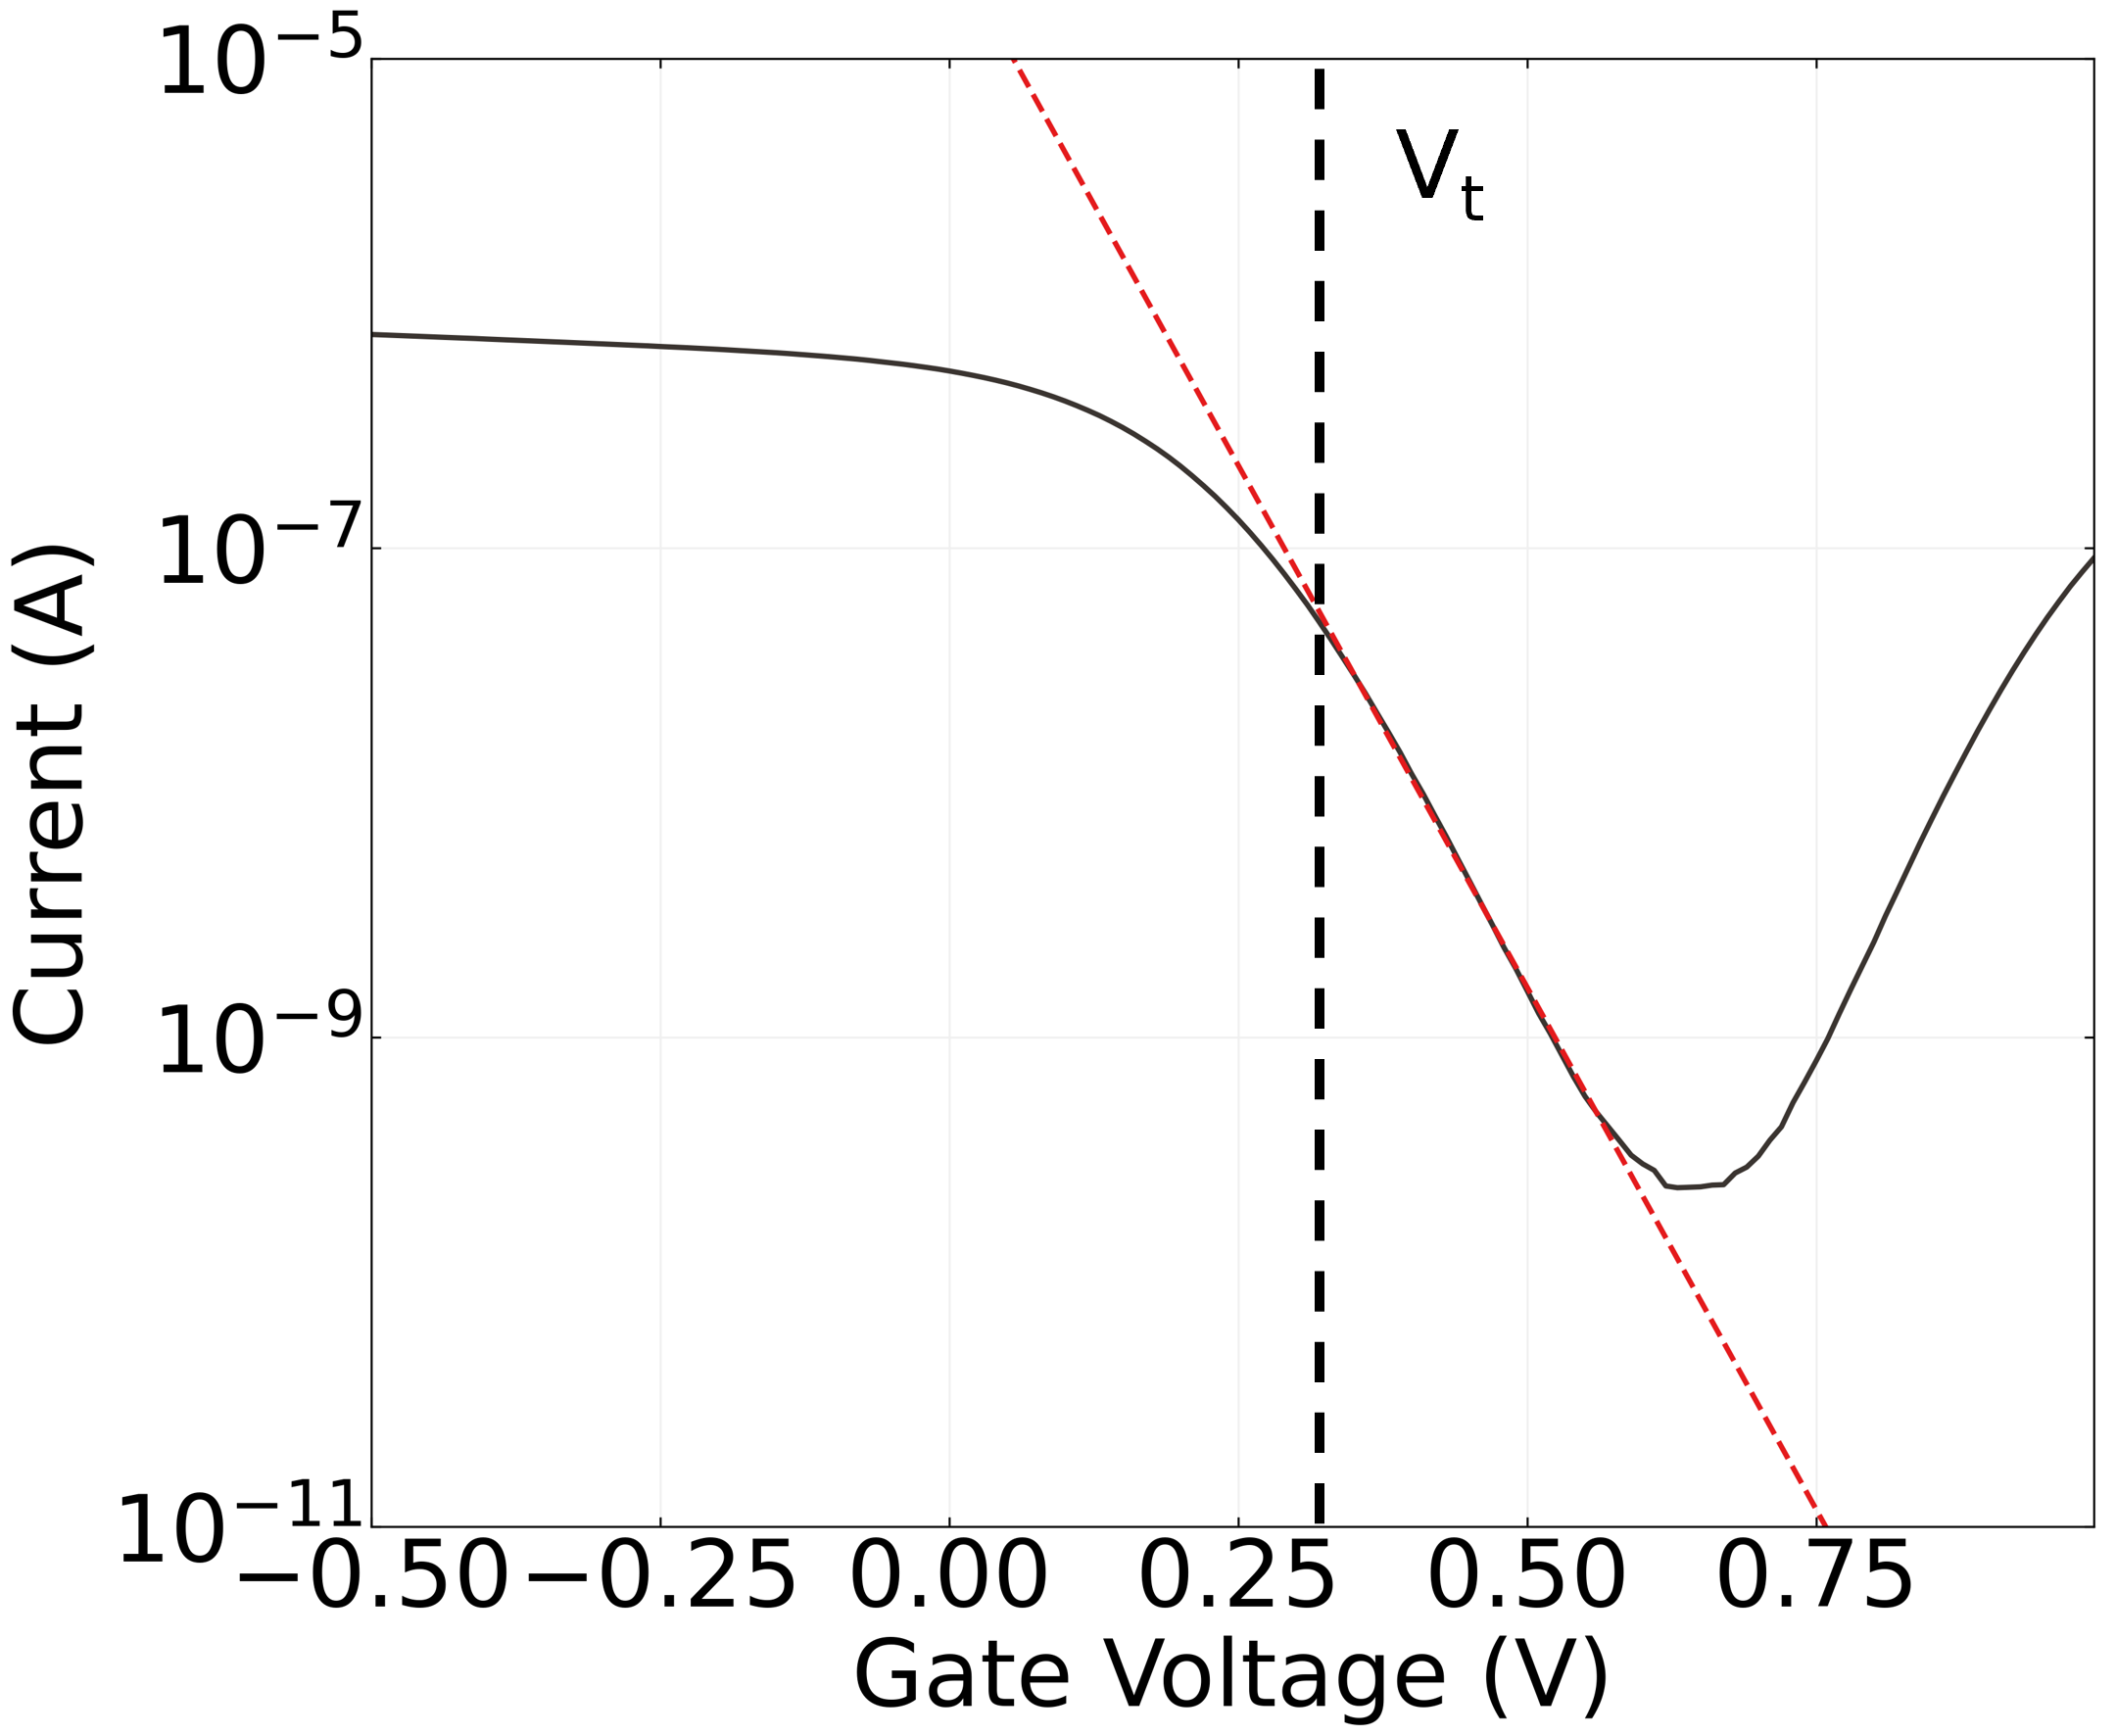
\includegraphics[width=0.45\textwidth,height=\textheight]{figures/ch2/NTQ31C5ch1subthreshold_slope_alt.png}

}

\caption{\label{fig-subthreshold-slope}A carbon nanotube network
transfer sweep with \(V_{ds}\) = 100 mV on a logarithmic scale.
Threshold voltage is shown with a black dotted line, while subthreshold
slope is shown with a red dotted line.}

\end{figure}

The subthreshold slope
\(S = d\textrm{log}_{10}(I_{d})/dV_g|_{\textrm{max}}\) is a measure of
how rapidly a transistor approaches the minimum current \(I_{off}\). The
subthreshold slope is often referred to using its reciprocal value, the
subthreshold swing, which is equivalent to the change in \(V_g\)
required to change \(I_d\) by one order of magnitude. This figure of
merit is strongly related to the gate capacitance of the device. As the
slope exponentially approaches the off current in the subthreshold
regime, it can be fitted with a linear trendline on a logarithimic
scale. \autocite{Sze2006,Petti2016}. A linear trendline fitted to the
logarithm of the subthreshold regime is shown in
Figure~\ref{fig-subthreshold-slope}, where the gradient corresponds to
subthreshold slope. A high subthreshold slope exceeding than 10
decades/V is preferred for reduced power consumption of the working
sensor device \autocite{Petti2016}. The subthreshold slope of the
transfer sweep in Figure~\ref{fig-subthreshold-slope} is 8 decades/V.
Heller \emph{et al.} and Gao \emph{et al.} found that sensor devices
showed better signal-to-noise ratio when gated in the subthreshold
regime, as small voltage changes in response to analyte led to
exponential current changes along the subthreshold slope
\autocite{Heller2009,Gao2010}.

\hypertarget{sec-CNT-sensing-mechanisms}{%
\subsection{Sensing}\label{sec-CNT-sensing-mechanisms}}

As all atoms are at the surface of the carbon nanotube structure,
nanotubes are very sensitive to their surroundings and easily modified,
making them useful in biosensor applications
\autocite{Cao2009,Yao2021,Shkodra2021}. The chirality and diameter of a
carbon nanotube affects both its coupling with the gate and its surface
chemistry, which determines the sensing mechanisms available to a single
CNT. Only s-CNTs can be electrostatically gated; m-CNTs, bent nanotubes
and larger diameter nanotubes are typically more reactive
\autocite{Cao2009,Zhao2012,Chhikara2013,Li2023}; and the nanotube
chirality (\(n,m\)) can determine the strength of binding to DNA in a
base sequence-dependent manner \autocite{Rouhi2011a}. Carbon nanotubes
have been used for vapour-phase sensing since 2000, when Kong \emph{et
al.} found that the resistance over a single CNT channel was modified
when exposed to gas molecules like NO\(_2\) and NH\(_3\)
\autocite{Kong2000}. Carbon nanotubes have been used to detect the
presence of analyte down to the parts per billion level in a variety of
gas sensor applications \autocite{Chen2019,Yao2021}. However, in
general, the specificity of such a sensor is low, as nanotubes respond
to many different analytes in a similar manner. To enhance specificity,
surface functionalisation is often performed using either inorganic or
biological materials, such as enzymes, antibodies, aptamers and proteins
\autocite{Cao2009,Shkodra2021,Yao2021}.

For carbon nanotube network transistors, sensing mechanisms include
electrostatic gating, charge transfer, Schottky barrier modulation,
modulation of channel capacitance relative to the electrolyte and charge
scattering. Response mechanisms may take place at the gate, the
junctions between channel and contact, or at the semiconductor channel
\autocite{Heller2008,Battie2011,Boyd2014,Tran2016,Li2023}. Modification
of the channel-metal Schottky barrier can dominate sensing activity, and
this can complicate the identification of mechanisms underlying the
sensing behaviour \autocite{Cao2009,Boyd2014,Schroeder2019}. The
encapsulation layer shown in Figure~\ref{fig-gating-schematics} is added
to separate the electrodes from the channel-metal junction and prevent
these responses \autocite{Heller2008,Shkodra2021}. In an encapsulated
device, the predominant sensing mechanism is either charge transfer from
the analyte to channel \autocite{Allen2007,Battie2011} or electrostatic
gating \autocite{Heller2008}. The charge transfer mechanism involves
direct addition of charge carriers to the channel, while the gating
mechanism results from a nearby charge inducing an opposite polarity
charge in the channel. Both changes alter the relationship between
\(V_g\) and \(I_d\) and shift the carrier threshold voltage(s)
\autocite{Tran2016,Shkodra2021,Li2023}. Modulation of Schottky and other
potential barriers present in the network may also make a significant
contribution to sensing responses, especially when a network is close to
its percolation threshold \autocite{Boyd2014,Murugathas2019}.

\hypertarget{summary}{%
\section{Summary}\label{summary}}

Graphene and carbon nanotube network field-effect transistors were
explored as the transducer element for vapour-phase biosensors due to
their low cost, small size and high sensitivity. Important device
parameters of the graphene and carbon nanotube network FETs include
transconductance, on-off ratio, gate leakage currents, current
hysteresis, threshold voltage and sub-threshold slope. The voltage
corresponding to the Dirac point (or points) of graphene is another
important figure of merit for graphene field-effect transistors. Various
attributes of the morphology of graphene and carbon nanotube networks
contribute to the unique electrical and sensing properties exhibited by
these transistors, including graphene folds and junctions between
nanotubes of different chirality. Research continues into optimising the
device morphology of thin-film FETs for maximum sensitivity, where the
the use of monolayer graphene and highly-purified s-CNT networks for the
thin-film are more recent developments in the field. Further exploration
of the relationship between thin-film morphology and transistor
characteristics can be found in \textbf{?@sec-pristine-characteristics}.

Although the sensitivity of these thin-film transistors is
well-established, the ability of these sensors to detect specific
compounds is a more recent area of exploration. In the past few decades,
a focus of investigation has been chemical and biological decoration of
these transistors to produce selective responses to compounds of
interest. The previous use of thin-film transistors functionalised with
odorant receptors to produce a specific sensing response is discussed in
detail in Chapter~\ref{sec-iOR-sensors}. There is also ongoing debate
regarding the precise mechanisms underlying sensing responses from these
transducers, particularly with respect to detection of vapour-phase or
gaseous compounds. A discussion of vapour-phase sensing with pristine
carbon nanotube thin-film transistors can be found in
\textbf{?@sec-pristine-characteristics}.

\bookmarksetup{startatroot}

\hypertarget{sec-iOR-sensors}{%
\chapter{Biosensing with Insect Odorant
Receptors}\label{sec-iOR-sensors}}

\hypertarget{sec-biosensing-transducers}{%
\section{Introduction}\label{sec-biosensing-transducers}}

In Chapter~\ref{sec-thin-film-transistors}, it was established that as
carbon nanotubes and graphene are extremely sensitive and are easily
modified with biomaterials, they are a highly suitable platform for
biosensing \autocite{Kauffman2008,Ohno2010}. In the early 2000s, it was
established that sensitive and selective biosensors could be created by
modifying a carbon nanotube field-effect transistor channel with protein
receptors \autocite{Chen2003,Kauffman2008}. In the following two
decades, a wide range of other biological receptors have been attached
to carbon nanotube FETs and graphene FETs for the creation of
biosensors, including enzymes \autocite{Lee2009,Zhang2015a,Dudina2019},
antibodies \autocite{Kim2008,Jin2015,Tsang2019} and aptameric DNA
\autocite{Maehashi2007,Gao2016,Nguyen2021}. These miniaturised `lab on a
chip' devices are of particular interest due to their reliability, low
cost, rapid use time, simple operation and small size compared with more
traditional biological analysis methods
\autocite{Kauffman2008,Khan2020}. It is hoped that such sensors could be
deployed outside the laboratory in a range of front-line settings which
require rapid and reliable detection
\autocite{Dung2018,Yang2018,Kim2022a}.

Rapid developments in this biosensor technology and parallel
developments in the understanding of animal olfaction led to these
transistors being used in bioelectronic nose applications from the late
2000s onwards \autocite{Yoon2009,Jin2012,Lee2012b,Park2012}.
`Bioelectronic nose' is a general term dating back to 1961, which refers
to the use of an biologically-modified electronic array to detect
specific odor traces in a highly selective and sensitive manner. As the
name suggests, the signals from this system mimic the electrochemical
signals received by olfactory neurons in an animal nose
\autocite{Glatz2011,Dung2018}. A biomimetic approach to bioelectronic
nose development couples the CNT FET or GFET signal-amplifying
transducer element with sensitive components of the animal olfactory
system. These components include olfactory cells \autocite{Wang2007},
odorant binding proteins (OBPs) \autocite{Larisika2015,Kotlowski2018}
and odorant receptor proteins (olfactory receptors, ORs)
\autocite{Yang2018,Murugathas2020}. An bioelectronic nose can discern
specific volatile odors in the air at low parts-per-trillion
concentrations, performance which is far superior to the human nose and
the best available gas sensor technology
\autocite{Lee2010,Moon2020,Terutsuki2020}. The aim for novel
olfactory-based electronic biosensors is to match or surpass this level
of selective accuracy
\autocite{Glatz2011,Kwon2015,Dung2018,Bohbot2020,Kim2022a}.

\hypertarget{sec-odorant-receptors-biosensors}{%
\section{Odorant Receptors in Field-Effect Transistor
Biosensors}\label{sec-odorant-receptors-biosensors}}

\hypertarget{sec-odorant-receptors}{%
\subsection{Odorant Receptors}\label{sec-odorant-receptors}}

Odorant receptors (ORs) are an essential part of the olfactory systems
of most animals, including humans. ORs let us distinguish between
thousands of odors \autocite{Buck1991,Dung2018,Yang2018,Kim2022a}.
Vertebrate odorant receptors are part of a group of seven-transmembrane
proteins known as G-protein coupled receptors (GPCRs)
\autocite{Buck1991,Glatz2011,Dung2018,Wicher2021}. Compounds entering a
vertebrate nose selectively bind to specific odorant receptors, which
undergo a change in conformation \autocite{Dung2018,Kim2022a}. The
binding process leads to activation and dissociation of the G-protein
within the neuronal cell. Intracellular signalling events triggered by
G-protein dissociation are converted to an action potential which is
then transmitted to the brain \autocite{Buck1991,Glatz2011,Zhang2021}.
The combination of activated receptors is then interpreted as a specific
odor \autocite{Sato2014,Kwon2015,Hurot2020,Kim2022a}. Odorant receptors
may be activated by a few or many target (or `agonist') compounds. The
target compounds are determined by subtle differences in OR amino acid
composition \autocite{Carraher2015,Yang2018,Goodwin2021}. An
`antagonist' compound may inhibit the response of a receptor to other
compounds \autocite{Lee2012,Carraher2015}. Compounds which trigger a
strong signal from a specific odorant receptor are often referred to as
`positive ligands' for that receptor, while those that cause no response
are `negative ligands'
\autocite{Murugathas2019a,Murugathas2020,Yoo2022}.

\hypertarget{sec-artificial-membranes}{%
\subsection{Artificial Membranes}\label{sec-artificial-membranes}}

Odorant receptors are transmembrane proteins, which are insoluble and
tend to aggregate and oligomerise in solution \autocite{Nath2007}. They
therefore require stabilisation from either a specific detergent
environment or a membrane layer to preserve their structure and function
when solubilised \autocite{Fruh2011,Dung2018}. Odorant receptors can be
expressed and isolated using heterologous cell systems, where a host
cell replicates a protein from transfected RNA or DNA material
\autocite{Glatz2011,Dung2018}. The most commonly used expression cells
are human embryonic kidney (HEK) cells \autocite{Lim2014,Ahn2020},
\emph{E. Coli} bacteria \autocite{Yang2017,Yang2018} and \emph{S.
cerevisiae} (baker's yeast) \autocite{Bohbot2020}. The cell membrane can
then be used directly in a sensor \autocite{Dung2018}. Alternatively,
odorant receptors can be embedded in an artificial lipid membrane format
that mimics the native cell membrane \autocite{Nath2007}. These
membranes can be produced in large numbers and remain in storage for
much longer than live cells \autocite{Goldsmith2011,Lim2015}. Lipid
membranes are constructed from phospholipid molecules, which comprise of
a small, hydrophilic, polar `head' and long, hydrophobic, non-polar
`tail' \autocite{Bose2021,Ramadon2022}. These artificial membranes
include detergent micelles, nanovesicles (including liposomes), and
nanodiscs \autocite{Yang2018,Moon2020}. The small size of these
artificial membranes makes them appropriate for use with
nanomaterial-based transducers \autocite{Lim2015,Dung2018}.

\begin{figure}

{\centering 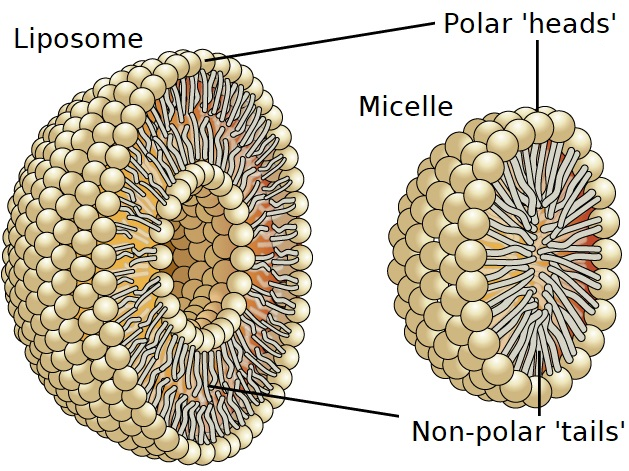
\includegraphics[width=0.53\textwidth,height=\textheight]{figures/ch3/OSC_Microbio_07_03_micelle_edit.png}

}

\caption{\label{fig-micelle}Liposomes and micelles are made up of a
lipid membrane, which acts as a substitute for the cell membrane
\emph{in vitro}. The polar, hydrophilic `heads' and non-polar,
hydrophobic `tails' of the component phospholipids are indicated.
Adapted from \autocite{Micelle}.}

\end{figure}

A nanovesicle is a nanoscopic spherical bilayer fluid sac. There are
various types of artificial nanovesicles, including liposomes,
ethosomes, transfersomes, niosomes and phytosomes. The type of
nanovesicle depends on its chemical makeup \autocite{Ramadon2022}. For
example, a liposome is made up of phospholipid and cholesterol, and can
consist of one or more concentric amphiphilic bilayers. The liposome can
contain hydrophobic compounds within the bilayer due to hydrophobic
interactions, while hydrophilic compounds are held within the vesicle
core or interior \autocite{Nath2007,Ramadon2022}. A nanovesicle can be
used solely as a format to protect membrane proteins
\autocite{Murugathas2020}, or with the addition of integrated ion
channels, can mimic the operation of a cell \emph{in vivo}, with
intracellular signalling pathways triggered by the membrane proteins
\autocite{Lim2015}. Nanomicelles (or simply micelles) are also
nanoscopic and spherical, but unlike nanovesicles have no inner fluid
sac \autocite{Nath2007,Bose2021}. Micelles self-assemble when
phospholipid is mixed with detergent. The surface of the micelle is made
up of the hydrophilic detergent and phospholipid heads, while the
internal core is made up of the hydrophobic phospholipid tail
\autocite{Nath2007}. Hydrophobic compounds can be contained within the
core of the micelle \autocite{Bose2021}. Figure~\ref{fig-micelle}
illustrates the difference between the liposome and micelle structures.

\begin{figure}

{\centering 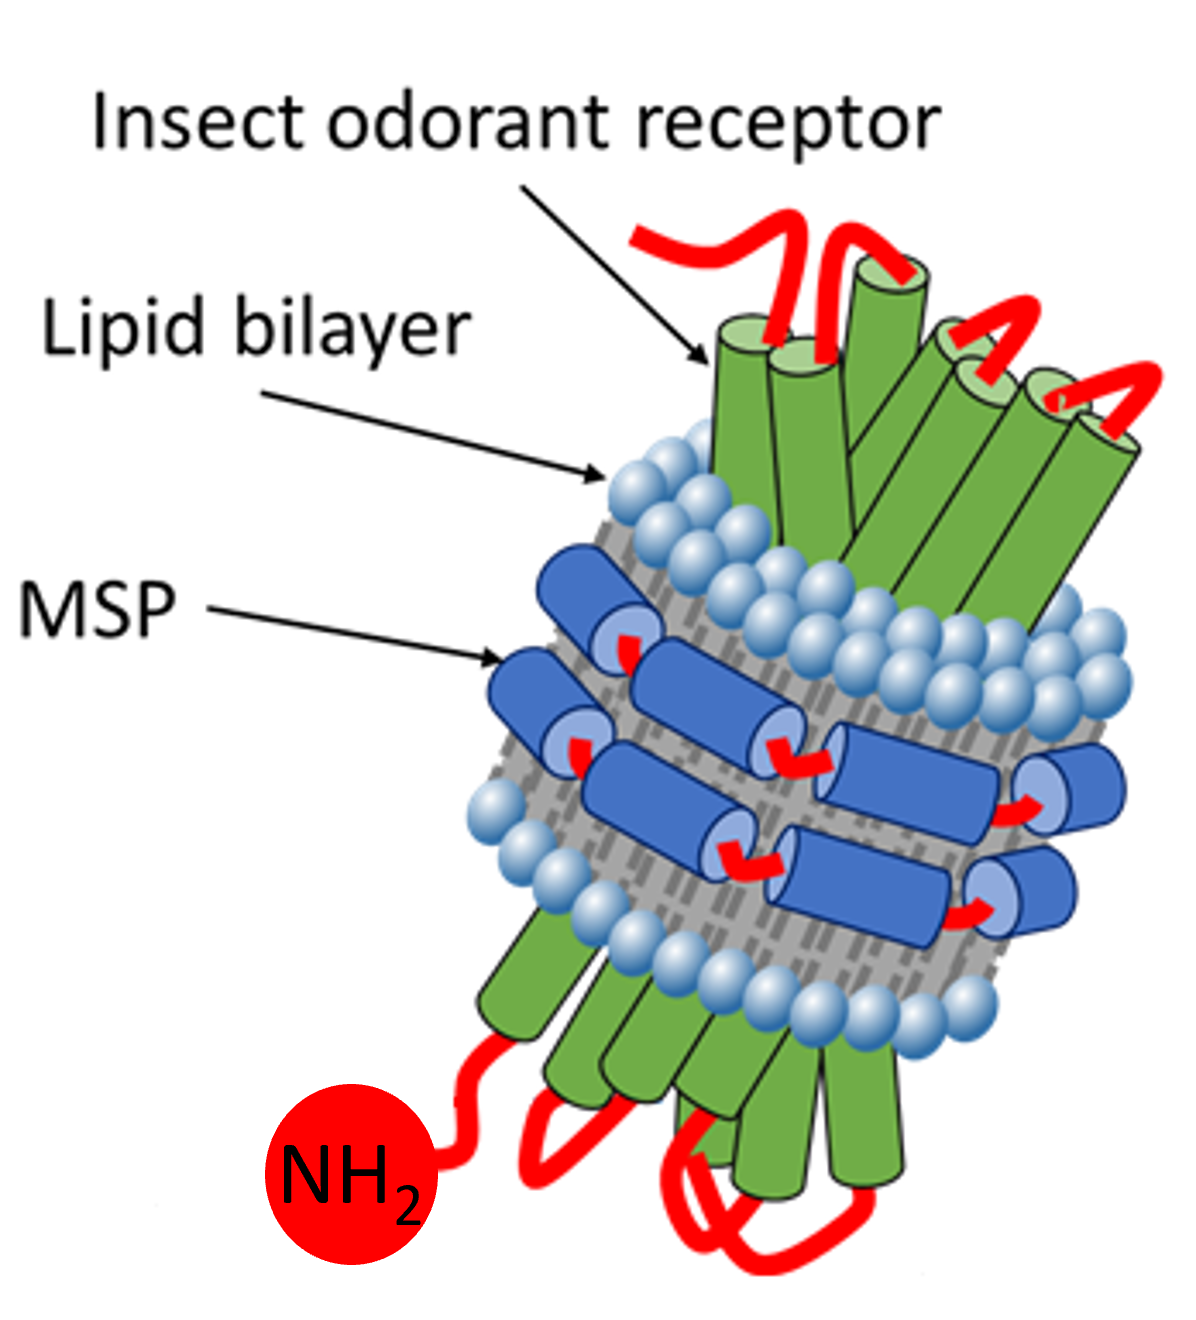
\includegraphics[width=0.4\textwidth,height=\textheight]{figures/ch3/iOR_nanodisc.png}

}

\caption{\label{fig-msp-iOR-nanodisc}A nanodisc containing an insect
odorant receptor transmembrane protein. The amine group shown is the
odorant receptor N-terminus. Reproduced with permission from
\autocite{Murugathas2019a}.}

\end{figure}

Nanodiscs have emerged as a model membrane candidate which has many
advantages over the more traditional nanovesicle and micelle formats.
The nanodisc is a disc-shaped lipid bilayer encompassed by an membrane
scaffold protein (MSP) \autocite{Nath2007,Bayburt2010,Yang2018}. The
amphiphilic membrane scaffold protein protects the exposed, strongly
hydrophobic side chains of the nanodisc in an aqueous environment
\autocite{Fruh2011,Yang2018}. Unlike liposomes and micelles, there is
little variation between the size of individual nanodiscs due to
constraints placed on the bilayer by the encompassing scaffold protein
used, meaning greater consistency within and between membrane batches
\autocite{Nath2007,Fruh2011}. Nanodiscs have also been found to be
significantly less prone to non-specific binding (see
Section~\ref{sec-non-specific-binding}) than micelles
\autocite{Fruh2011}. Another advantage of nanodiscs is that the membrane
scaffold protein can be attached to biosensor surfaces at specific
affinity tags, for example, the scaffold protein hexahistidine tag
(his-tag) \autocite{Bayburt2010,Fruh2011}. Depending on the type of MSP
used, a nanodisc measures between 10-20 nm across and can hold either a
single or several odorant receptors \autocite{Nath2007,Bayburt2010}. The
protein coating of the nanodisc makes it particularly stable. The
stability of nanodiscs means they can be used to produce particularly
reliable and long-lived biosensor devices
\autocite{Goldsmith2011,Yang2018,Moon2020,Cheema2021}.

\hypertarget{sec-sensor-types}{%
\subsection{Sensor Functionalisation}\label{sec-sensor-types}}

For a bioelectronic nose to operate, sufficient coupling must exist
between the bioreceptor element and the sensor transducer. Odorant
receptors can be directly attached by physical adsorption; however, this
approach is difficult to control, and can result in weak coupling
between the odorant receptors and the transducer
\autocite{Kwon2015,Dung2018,Bohbot2020}. Alternatively, a bifunctional
linker element may mediate the attachment between functional groups of
the bioreceptor and the carbon-ring surface of the transducer in a
biochemical process referred to as functionalisation
\autocite{Star2003a}. In this thesis, the amino functional group is of
particular interest, but there are many other nucleophilic functional
groups available for binding, including carboxyls, hydroxyls,
thiols/sulfhydryls, phenols, imidazoles and so on
\autocite{Fruh2011,Dung2018}. The linker chemical interacts with the
transducer either through stronger covalent bonding or weaker
non-covalent bonding. The relative advantages and disadvantages of each
type of receptor immobilisation can be found in
Table~\ref{tbl-functionalisation-types}, while a more thorough
comparison of covalent and non-covalent linker functionalisation can be
found in \textbf{?@sec-noncovalent-functionalisation}.

\hypertarget{tbl-functionalisation-types}{}
\begin{longtable}[t]{>{\raggedright\arraybackslash}p{5.4cm}>{\raggedright\arraybackslash}p{1.45cm}>{\raggedright\arraybackslash}p{1.3cm}>{\raggedright\arraybackslash}p{1.45cm}>{\raggedright\arraybackslash}p{1.3cm}>{\raggedright\arraybackslash}p{1.3cm}}
\caption{\label{tbl-functionalisation-types}A comparison of the advantages and disadvantages of different approaches
for immobilising odorant receptors onto carbon nanotube or graphene
transducers. Simplicity \(-\) minimal cost, time and effort required for
functionalisation; Synergy \(-\) receptor attachment which does not
negatively impact transducer operation or receptor activity; Stability
\(-\) successful operation over a long time and under a range of
conditions; Specificity \(-\) receptor attachment in a controlled and
directional manner; Strength \(-\) strong receptor-transducer binding. }\tabularnewline

\toprule
Attachment Type & Simplicity & Synergy & Specificity & Stability & Strength\\
\midrule
Direct Adsorption & High & Medium & Low & Low & Low\\
Linker, covalently tethered & Medium & Low & High & High & High\\
Linker, non-covalently tethered & Medium & High & Medium & Medium & Medium\\
\bottomrule
\end{longtable}

Table~\ref{tbl-or-biosensors} summarises all published odorant-receptor
functionalised carbon nanotube and graphene field-effect
transistor-based sensors to date. The majority of published works on
this topic come from the Tai Hyun Park group at Seoul National
University. The Park group has mainly focused on CNT FETs functionalised
with human odorant receptors, but has used a range of different covalent
and non-covalent transducer immobilisation techniques when producing the
sensors. Dog and mouse odorant receptors have also been used, by the
Park group and by Goldsmith \emph{et al.} respectively. As far as the
author knows, the Plank group at Te Herenga Waka \(-\) Victoria
University of Wellington is the only group to have produced carbon
nanotube and graphene field-effect transistors functionalised with
insect odorant receptors. The behaviour of insect odorant receptors is
significantly different to that of vertebrate odorant receptors, and
their behaviour in sensor applications is currently not well understood.
The distinction between vertebrate and insect odorant receptors is
discussed in more depth in Section~\ref{sec-insect-OR-biosensors}.

Three functionalisation linkers were used by both the Park group and a
secondary research group: non-covalently attached glutaraldehyde
(GA)-conjugated 1,5-diaminonaphthalene (DAN)
\autocite{Kwon2015,Goodwin2021}, non-covalently attached
1-pyrenebutanoic acid N-hydroxysuccinimide ester (PBASE)
\autocite{Murugathas2020,Yoo2022}, and covalently attached
nickel-nitrilotriacetic acid (Ni-NTA) modified diazonium salt
\autocite{Goldsmith2011,Son2017}. The bonding between the linker
molecule and receptor element is typically covalent, regardless of the
type of bonding that exists between linker and transducer.
Interestingly, no single paper compares multiple possible
functionalisation techniques directly, making it difficult to assess the
relative quality of various attachment methods. The limit of detection
(LOD) could be used as a rough measure of quality. The functionalisation
procedure resulting in the lowest limit of detection used was
non-covalent \autocite{Park2012}. However, the quoted LOD is highly
variable across the non-covalently functionalised devices. Furthermore,
non-covalent functionalisation of odorant receptors has never been used
for vapour sensing. The next section further explores the sensing
behaviour of biosensors functionalised with the most commonly-used
protocols.

\newpage
\thispagestyle{empty}
\KOMAoptions{paper=landscape,pagesize}

\hypertarget{tbl-or-biosensors}{}
\begin{longtable}[]{@{}lllllll@{}}
\caption{\label{tbl-or-biosensors}Summary of past fabrication methods
for odorant receptor-functionalised carbon nanotube and graphene
biosensors.}\tabularnewline
\toprule\noalign{}
Attachment & Attachment Method & References & Transducer & OR Type & OR
Format & LOD \\
\midrule\noalign{}
\endfirsthead
\toprule\noalign{}
Attachment & Attachment Method & References & Transducer & OR Type & OR
Format & LOD \\
\midrule\noalign{}
\endhead
\bottomrule\noalign{}
\endlastfoot
Non-covalent & Vacuum-drying & Kim, 2009. \cite{Kim2009a} & CNTFET &
Human & Cell membrane & 100 fM \\
& DMT-MM & Yoon, 2009. \cite{Yoon2009} & CNTFET & Human & Cell membrane
& 10 fM \\
& PDL & Jin, 2012. \cite{Jin2012} & CNTFET & Human & Nanovesicles & 1
fM \\
& & Park, 2012. \cite{Park2012a} & CNTFET & Dog & Nanovesicles & 1 fM \\
& & Lim, 2014. \cite{Lim2014} & CNTFET & Human & Nanovesicles & 10 fM \\
& & Lim, 2015. \cite{Lim2015} & CNTFET & Human & Nanovesicles & 1 fM \\
& & Son, 2015. \cite{Son2015} & CNTFET & Human & Nanovesicles & 10
ng/L \\
& & Ahn, 2015. \cite{Ahn2015} & CNTFET & Human & Nanovesicles & 1 fM \\
& GA-conjugated DAN & Park, 2012. \cite{Park2012} & GFET & Human & Cell
membrane & 0.04 fM \\
& & Lee, 2012. \cite{Lee2012b} & CNTFET & Human & Cell membrane & 1
fM \\
& & Kwon, 2015. \cite{Kwon2015} & GFET & Human & Cell membrane & 0.1
fM \\
& & Goodwin, 2021. \cite{Goodwin2021} & GFET & Human & Cell membrane &
0.5 pM \\
& PBASE & Murugathas, 2019. \cite{Murugathas2019a} & CNTFET &
\textit{Insect} & Nanodiscs & 1 fM \\
& & Murugathas, 2020. \cite{Murugathas2020} & GFET & \textit{Insect} &
Nanovesicles, Nanodiscs & 1 fM \\
& & Ahn, 2020. \cite{Ahn2020} & GFET & Human & Nanovesicles & 100 fM \\
& & Yoo, 2022. \cite{Yoo2022} & CNTFET & Human & Micelles & 1 fM \\
Covalent & Diazonium salt/Ni-NTA & Goldsmith, 2011. \cite{Goldsmith2011}
& CNTFET & Mouse & Micelles, Nanodiscs & \textasciitilde7 ppb \\
& & Son, 2017. \cite{Son2017} & CNTFET & Human & Micelles & 10 fM \\
& Half-v5 mouse Ab & Lee, 2018. \cite{Lee2018} & CNTFET & Human &
Nanodiscs & 1 fM \\
\end{longtable}

\newpage
\KOMAoptions{paper=portrait,pagesize}

\hypertarget{sec-biosensor-methods}{%
\subsection{Sensing Behaviour}\label{sec-biosensor-methods}}

\begin{figure}

\begin{minipage}[t]{0.03\linewidth}

{\centering 

\raisebox{-\height}{


\includegraphics{figures/(a).png}

}

}

\end{minipage}%
%
\begin{minipage}[t]{0.01\linewidth}

{\centering 

~

}

\end{minipage}%
%
\begin{minipage}[t]{0.45\linewidth}

{\centering 

\raisebox{-\height}{

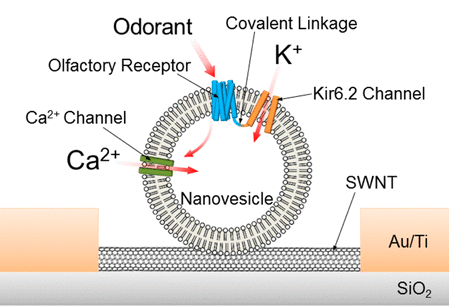
\includegraphics{figures/ch3/ion-channel-nanovesicle-lim2015.png}

}

}

\end{minipage}%
%
\begin{minipage}[t]{0.01\linewidth}

{\centering 

~

}

\end{minipage}%
%
\begin{minipage}[t]{0.03\linewidth}

{\centering 

\raisebox{-\height}{

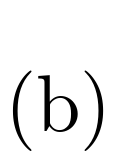
\includegraphics{figures/(b).png}

}

}

\end{minipage}%
%
\begin{minipage}[t]{0.01\linewidth}

{\centering 

~

}

\end{minipage}%
%
\begin{minipage}[t]{0.45\linewidth}

{\centering 

\raisebox{-\height}{

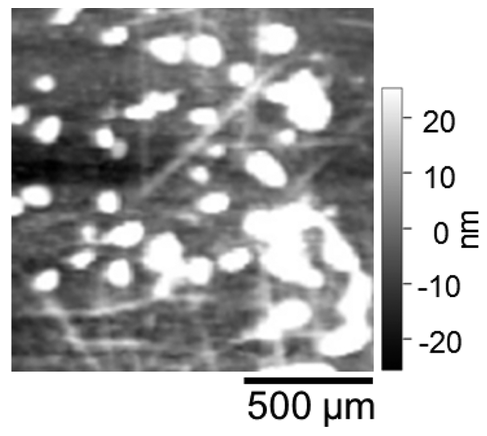
\includegraphics{figures/ch3/afm-nanovesicle-lim2015.png}

}

}

\end{minipage}%
%
\begin{minipage}[t]{0.01\linewidth}

{\centering 

~

}

\end{minipage}%
\newline
\begin{minipage}[t]{0.03\linewidth}

{\centering 

\raisebox{-\height}{


\includegraphics{figures/(c).png}

}

}

\end{minipage}%
%
\begin{minipage}[t]{0.01\linewidth}

{\centering 

~

}

\end{minipage}%
%
\begin{minipage}[t]{0.45\linewidth}

{\centering 

\raisebox{-\height}{

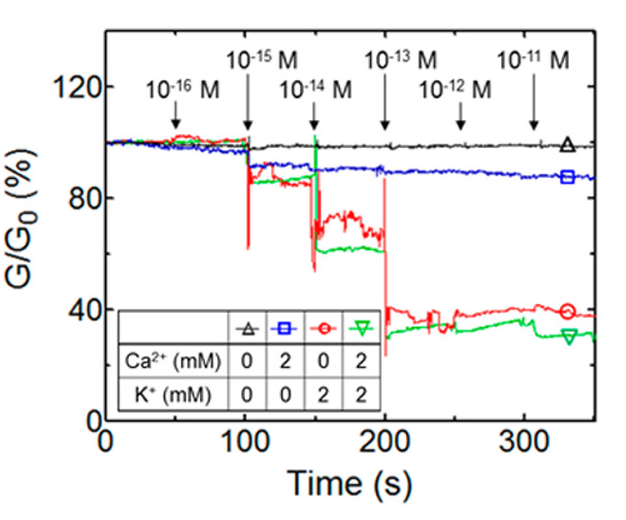
\includegraphics{figures/ch3/nanovesicle-amyl-butyrate-1-lim2015.png}

}

}

\end{minipage}%
%
\begin{minipage}[t]{0.01\linewidth}

{\centering 

~

}

\end{minipage}%
%
\begin{minipage}[t]{0.03\linewidth}

{\centering 

\raisebox{-\height}{

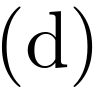
\includegraphics{figures/(d).png}

}

}

\end{minipage}%
%
\begin{minipage}[t]{0.01\linewidth}

{\centering 

~

}

\end{minipage}%
%
\begin{minipage}[t]{0.45\linewidth}

{\centering 

\raisebox{-\height}{

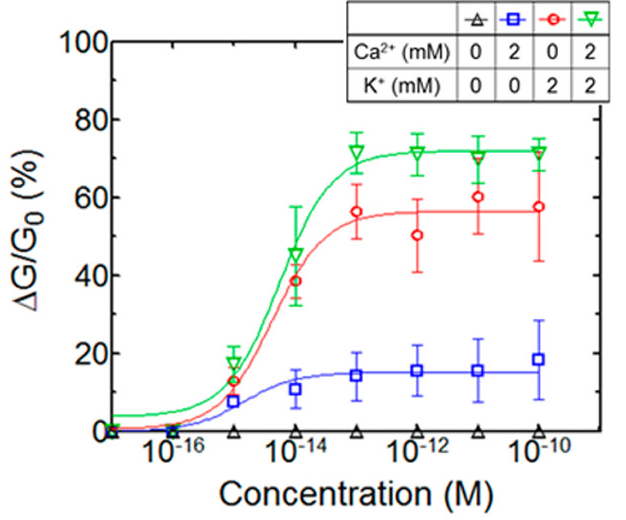
\includegraphics{figures/ch3/nanovesicle-amyl-butyrate-2-lim2015.png}

}

}

\end{minipage}%
%
\begin{minipage}[t]{0.01\linewidth}

{\centering 

~

}

\end{minipage}%

\caption{\label{fig-lim-ion-channel}Schematics detailing the
nanovesicle-based carbon nanotube field-effect biosensor of Lim \emph{et
al.} (a) shows a schematic of the different elements and signalling
pathways present in the sensor, (b) shows an atomic force microscope
image of the functionalised device, (c) shows real-time conductance
changes resulting from amyl butyrate additions to the electrolyte gate
against relevant controls, and (d) shows the dose-dependent response
pattern to amyl butyrate. Reproduced with permission from
\autocite{Lim2015}.}

\end{figure}

Nanovesicle-based odorant receptor biosensors can be used to couple a
vertebrate odorant receptor with an ion channel, where the presence of
analyte leads to a flow of ions into an olfactory cell
\autocite{Lim2015,Dung2018}. Lim \emph{et al.} functionalised a CNT FET
with nanovesicles featuring a human odorant receptor hOR2AG1 covalently
coupled with a potassium ion channel, alongside an endogenous calcium
ion channel, as shown in Figure~\ref{fig-lim-ion-channel} (a). These
nanovesicles were attached to the random carbon nanotube network through
a charge-charge interaction with poly-D-lysine, demonstrated with the
atomic force microscope image shown in Figure~\ref{fig-lim-ion-channel}
(b). Binding of amyl butyrate to hOR2AG1 causes the OR to change
conformation, opening the coupled potassium ion channel and gating the
transistor channel. The real-time signal responses associated with amyl
butyrate binding in the electrolyte environment are shown in
Figure~\ref{fig-lim-ion-channel} (c). Intracellular signalling by the
odorant receptors means that target binding also opens the calcium ion
channel, so a response can be seen when only calcium ions are present.
Without potassium or calcium ions present, ion inflow cannot occur, so
no conductance change is observed. Figure~\ref{fig-lim-ion-channel} (d)
shows the dose dependent response to amyl butyrate in various
electrolytes \autocite{Lim2015}.

\begin{figure}

\begin{minipage}[t]{0.03\linewidth}

{\centering 

\raisebox{-\height}{


\includegraphics{figures/(a).png}

}

}

\end{minipage}%
%
\begin{minipage}[t]{0.04\linewidth}

{\centering 

~

}

\end{minipage}%
%
\begin{minipage}[t]{0.90\linewidth}

{\centering 

\raisebox{-\height}{

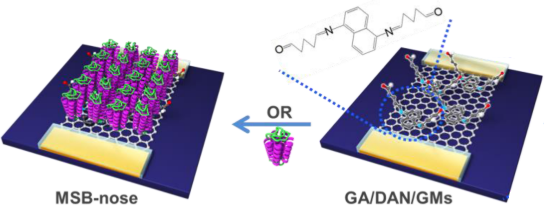
\includegraphics{figures/ch3/kwon2015-OR-graphene.png}

}

}

\end{minipage}%
%
\begin{minipage}[t]{0.04\linewidth}

{\centering 

~

}

\end{minipage}%
\newline
\begin{minipage}[t]{0.03\linewidth}

{\centering 

\raisebox{-\height}{

\includegraphics{figures/(b).png}

}

}

\end{minipage}%
%
\begin{minipage}[t]{0.01\linewidth}

{\centering 

~

}

\end{minipage}%
%
\begin{minipage}[t]{0.45\linewidth}

{\centering 

\raisebox{-\height}{

\includegraphics{figures/ch3/kwon2015_transfer.png}

}

}

\end{minipage}%
%
\begin{minipage}[t]{0.01\linewidth}

{\centering 

~

}

\end{minipage}%
%
\begin{minipage}[t]{0.03\linewidth}

{\centering 

\raisebox{-\height}{

\includegraphics{figures/(c).png}

}

}

\end{minipage}%
%
\begin{minipage}[t]{0.01\linewidth}

{\centering 

~

}

\end{minipage}%
%
\begin{minipage}[t]{0.45\linewidth}

{\centering 

\raisebox{-\height}{

\includegraphics{figures/ch3/kwon2015-amyl-butyrate.png}

}

}

\end{minipage}%
%
\begin{minipage}[t]{0.01\linewidth}

{\centering 

~

}

\end{minipage}%
\newline
\begin{minipage}[t]{0.03\linewidth}

{\centering 

\raisebox{-\height}{

\includegraphics{figures/(d).png}

}

}

\end{minipage}%
%
\begin{minipage}[t]{0.01\linewidth}

{\centering 

~

}

\end{minipage}%
%
\begin{minipage}[t]{0.45\linewidth}

{\centering 

\raisebox{-\height}{

\includegraphics{figures/ch3/kwon2015-helional.png}

}

}

\end{minipage}%
%
\begin{minipage}[t]{0.01\linewidth}

{\centering 

~

}

\end{minipage}%
%
\begin{minipage}[t]{0.03\linewidth}

{\centering 

\raisebox{-\height}{

\includegraphics{figures/(e).png}

}

}

\end{minipage}%
%
\begin{minipage}[t]{0.01\linewidth}

{\centering 

~

}

\end{minipage}%
%
\begin{minipage}[t]{0.45\linewidth}

{\centering 

\raisebox{-\height}{

\includegraphics{figures/ch3/kwon2015-dose.png}

}

}

\end{minipage}%
%
\begin{minipage}[t]{0.01\linewidth}

{\centering 

~

}

\end{minipage}%

\caption{\label{fig-kwon-multiplexed}Schematics showing the odorant
receptor-functionalised graphene field-effect biosensor of Kwon \emph{et
al.} (a) shows the functionalisation of odorant receptors onto graphene
using non-covalently attached GA-modified DAN linker; (b) compares
transfer characteristics of the device with graphene only (GM), graphene
with DAN linker (GM/DAN), and after modification with one of two
different ORs (hOR2AG1, hOR3A1); (c) shows the real-time responses of
the liquid-gated hOR2AG1-modified transistor (sub-SB2) to various
concentrations of amyl butyrate (AB) analyte; (d) shows the real-time
responses of the hOR3A1-modified transistor (sub-SB3) to various
concentrations of helional (HE) analyte; and (e) shows the
dose-dependent response curve corresponding to the sub-SB2 and sub-SB3
sensors. Reproduced with permission from \autocite{Kwon2015}.}

\end{figure}

Odorant receptors can also be expressed in the native cell membrane and
attached directly to the biosensor channel. Here, the changes in odorant
receptor conformation that result from analyte binding cause affects the
distance between charges on the odorant receptor and the transducer
channel, gating the channel \autocite{Kwon2015,Dung2018}. Kwon \emph{et
al.} functionalised graphene field-effect transistors with human odorant
receptors hOR2AG1 and hOR3A1 using non-covalently attached
1,5-diaminonaphthalene (DAN) modified with glutaraldehyde (GA) as a
linker, as shown in Figure~\ref{fig-kwon-multiplexed} (a). The odorant
receptors attach to the GA-modified DAN via a Schiff-base reaction
\autocite{Subasi2022}. OR attachment was demonstrated by SEM imaging as
well as a significant change in device resistance, shown in
Figure~\ref{fig-kwon-multiplexed} (b). Both hOR2AG1 and hOR3A1 showed
real-time responses to their corresponding target analyte at
sub-femtomolar concentrations, as shown in
Figure~\ref{fig-kwon-multiplexed} (c) and
Figure~\ref{fig-kwon-multiplexed} (d) respectively. No responses were
seen from linker-modified graphene to the same analyte additions. The
dose-dependent response curve of both these odorant receptor sensors is
shown in Figure~\ref{fig-kwon-multiplexed} (e). As in
Figure~\ref{fig-lim-ion-channel} (d), a Langmuir-type dose response
behaviour was seen, where a logarithmic increase in signal response is
observed for sub-femtomolar or femtomolar concentration analyte
additions, which gives way to saturation behaviour with picomolar
additions.

\begin{figure}

\begin{minipage}[t]{0.03\linewidth}

{\centering 

\raisebox{-\height}{

\includegraphics{figures/(a).png}

}

}

\end{minipage}%
%
\begin{minipage}[t]{0.01\linewidth}

{\centering 

~

}

\end{minipage}%
%
\begin{minipage}[t]{0.45\linewidth}

{\centering 

\raisebox{-\height}{

\includegraphics{figures/ch3/yoo2022-micelle-cnt.png}

}

}

\end{minipage}%
%
\begin{minipage}[t]{0.01\linewidth}

{\centering 

~

}

\end{minipage}%
%
\begin{minipage}[t]{0.03\linewidth}

{\centering 

\raisebox{-\height}{

\includegraphics{figures/(b).png}

}

}

\end{minipage}%
%
\begin{minipage}[t]{0.01\linewidth}

{\centering 

~

}

\end{minipage}%
%
\begin{minipage}[t]{0.45\linewidth}

{\centering 

\raisebox{-\height}{

\includegraphics{figures/ch3/yoo2022-AFM.png}

}

}

\end{minipage}%
%
\begin{minipage}[t]{0.01\linewidth}

{\centering 

~

}

\end{minipage}%
\newline
\begin{minipage}[t]{0.03\linewidth}

{\centering 

\raisebox{-\height}{

\includegraphics{figures/(c).png}

}

}

\end{minipage}%
%
\begin{minipage}[t]{0.01\linewidth}

{\centering 

~

}

\end{minipage}%
%
\begin{minipage}[t]{0.45\linewidth}

{\centering 

\raisebox{-\height}{

\includegraphics{figures/ch3/yoo2022-TX.png}

}

}

\end{minipage}%
%
\begin{minipage}[t]{0.01\linewidth}

{\centering 

~

}

\end{minipage}%
%
\begin{minipage}[t]{0.03\linewidth}

{\centering 

\raisebox{-\height}{

\includegraphics{figures/(d).png}

}

}

\end{minipage}%
%
\begin{minipage}[t]{0.01\linewidth}

{\centering 

~

}

\end{minipage}%
%
\begin{minipage}[t]{0.45\linewidth}

{\centering 

\raisebox{-\height}{

\includegraphics{figures/ch3/yoo2022-DMMP.png}

}

}

\end{minipage}%
%
\begin{minipage}[t]{0.01\linewidth}

{\centering 

~

}

\end{minipage}%
\newline
\begin{minipage}[t]{0.03\linewidth}

{\centering 

\raisebox{-\height}{

\includegraphics{figures/(e).png}

}

}

\end{minipage}%
%
\begin{minipage}[t]{0.01\linewidth}

{\centering 

~

}

\end{minipage}%
%
\begin{minipage}[t]{0.45\linewidth}

{\centering 

\raisebox{-\height}{

\includegraphics{figures/ch3/yoo2022-DMMP-2.png}

}

}

\end{minipage}%
%
\begin{minipage}[t]{0.01\linewidth}

{\centering 

~

}

\end{minipage}%
%
\begin{minipage}[t]{0.03\linewidth}

{\centering 

\raisebox{-\height}{

\includegraphics{figures/(f).png}

}

}

\end{minipage}%
%
\begin{minipage}[t]{0.01\linewidth}

{\centering 

~

}

\end{minipage}%
%
\begin{minipage}[t]{0.45\linewidth}

{\centering 

\raisebox{-\height}{

\includegraphics{figures/ch3/yoo2022-DMMP-3.png}

}

}

\end{minipage}%
%
\begin{minipage}[t]{0.01\linewidth}

{\centering 

~

}

\end{minipage}%

\caption{\label{fig-yoo-micelle}Schematics of the micelle-based carbon
nanotube field-effect transistor of Yoo \emph{et al.} (a) shows the
functionalisation of detergent micelles onto the carbon nanotube network
channel; (b) shows the same height profile across an atomic force
microscope image of the carbon nanotube network before and after
functionalisation with micelles using PBASE; (c) shows the liquid-gated
transfer characteristic of a device channel before and after
functionalisation with PBASE and micelles; (d) shows real-time responses
of the functionalised, liquid-gated channel to additions of dimethyl
methylphosphonate (DMMP) analyte; (e) shows the dose-dependent response
curve to DMMP; and (f) shows a control series demonstrating the
selective behaviour of the sensor, where EB is ethyl butyrate and AB is
amyl butyrate. Reproduced with permission from \autocite{Yoo2022}.}

\end{figure}

Biosensors have also been produced where odorant receptors are held in a
detergent micelle format instead of the native cell membrane. The
mechanism behind sensing is the same as for odorant receptors in the
cell membrane, where a conformational change in the odorant receptors
leads to channel gating \autocite{Dung2018,Yoo2022}. Yoo \emph{et al.}
functionalised random-network CNT FETs with detergent micelles which
contained human odorant receptor hOR2T7. PBASE was used as the linker
molecule, which attaches to the odorant receptor via its amine group and
non-covalently tethers it to the transducer, illustrated in
Figure~\ref{fig-yoo-micelle} (a). Successful immobilisation was
demonstrated by a raised atomic force microscope height profile after
receptor attachment (Figure~\ref{fig-yoo-micelle} (b)) and an on-current
drop in the liquid-gated transfer characteristics of the device
(Figure~\ref{fig-yoo-micelle} (c)). The sensor showed sharp real-time
responses to the addition of DMMP concentrations, as seen in
Figure~\ref{fig-yoo-micelle} (d). The dose dependence curve for DMMP
responses is shown in in Figure~\ref{fig-yoo-micelle} (e), again showing
a Langmuir-type response curve to successive DMMP additions. Various
analytes with a similar scent to DMMP were added at high concentrations
to the liquid-gate, shown in Figure~\ref{fig-yoo-micelle} (f). No
response was seen to any these additions, demonstrating the selectivity
of the sensor.

In the first study of this kind, Goldsmith \emph{et al.} demonstrated
that a single-CNT device functionalised with mOR174-9 odorant receptors
in either a micelle or nanodisc format could be used as a vapour-phase
biosensor. Micelle immobilisation was confirmed using atomic force
microscopy, as shown in Figure~\ref{fig-eugenol-responses} (a). The mOR
CNT FETs were exposed to nitrogen flow at 50\% relative humidity. The
conductance across the channel was measured while a specific
concentration of the positive ligand eugenol was added to the constant
flow for 100 s, then removed from the flow for 100 s. This cycle was
repeated five times. Figure~\ref{fig-eugenol-responses} (b) shows that a
\(\sim\) 9\% increase in current was observed during each cycle of
exposure to eugenol. The device still responded to eugenol cycles after
69 days of storage in 25\% (v/v) ethanol at 4°C. This persistent
activity may result from the long-lived nanodisc format used
\autocite{Goldsmith2011}. As far as the author knows, there is no
existing study which investigates whether this behaviour can be
replicated for insect odorant receptor devices. It is not clear that the
vertebrate odorant receptors used here can simply be substituted for
iORs for vapour-phase sensing. The difference between receptors is
discussed further in the subsequent section.

\begin{figure}

\begin{minipage}[t]{0.03\linewidth}

{\centering 

\raisebox{-\height}{

\includegraphics{figures/(a).png}

}

}

\end{minipage}%
%
\begin{minipage}[t]{0.01\linewidth}

{\centering 

~

}

\end{minipage}%
%
\begin{minipage}[t]{0.40\linewidth}

{\centering 

\raisebox{-\height}{

\includegraphics{figures/ch3/afm-nanodisc-goldsmith.png}

}

}

\end{minipage}%
%
\begin{minipage}[t]{0.01\linewidth}

{\centering 

~

}

\end{minipage}%
%
\begin{minipage}[t]{0.03\linewidth}

{\centering 

\raisebox{-\height}{

\includegraphics{figures/(b).png}

}

}

\end{minipage}%
%
\begin{minipage}[t]{0.01\linewidth}

{\centering 

~

}

\end{minipage}%
%
\begin{minipage}[t]{0.50\linewidth}

{\centering 

\raisebox{-\height}{

\includegraphics{figures/ch3/eugenol-goldsmith.png}

}

}

\end{minipage}%
%
\begin{minipage}[t]{0.01\linewidth}

{\centering 

~

}

\end{minipage}%

\caption{\label{fig-eugenol-responses}The functionalisation of mOR174-9
nanodiscs onto single-CNT field effect transistor vapour sensing use is
demonstrated with an atomic force microscope image in (a), while (b)
shows real-time responses of the sensor to 2 ppm eugenol vapour. The
response to eugenol on day 69 (red triangles) indicates that the device
retains the ability to respond to eugenol 10 weeks after
functionalisation. Reproduced with permission from
\autocite{Goldsmith2011}.}

\end{figure}

\hypertarget{sec-insect-OR-biosensors}{%
\section{Insect Odorant Receptor Field-Effect Transistor
Biosensors}\label{sec-insect-OR-biosensors}}

\hypertarget{insect-odorant-receptors}{%
\subsection{Insect Odorant Receptors}\label{insect-odorant-receptors}}

Insect odorant (or olfactory) receptors (iORs) are a diverse range of
odorant-sensitive seven-transmembrane proteins located in the dendrite
cells of insect sensory hairs, known as sensilla
\autocite{Clyne1999,Carraher2015,Brito2016,Wicher2021}. When volatile
compounds enter the sensilla, they are carried by odorant binding
proteins (OBPs) through an aqueous environment to the dendrite cells
\autocite{Carraher2015,Brito2016,Wicher2021}. These cells possess a
insect-specific set of `tuning' iORs alongside a generic co-receptor
known as `ORCO' (Odorant Receptor Co-Receptor)
\autocite{Carraher2015,Butterwick2018,Khadka2019,Wicher2021}. The ORCO
co-receptor is insensitive to target compounds (aside from synthetic
compounds like VUAA1). Instead, it couples with the tuning iOR to form a
non-selective, permeable ion channel
\autocite{Butterwick2018,Wicher2021}. When a compound binds to a tuning
iOR, the ion channel opens to allow cations to travel across the cell
membrane, activating intracellular signalling
\autocite{Smart2008,Wicher2008,Sato2008,Carraher2015,Brito2016,Butterwick2018,Wicher2021}.
The combination of resulting OR signals is sent to the insect brain for
interpretation as an odor. The tuning iORs respond to (or are inhibited
by) a huge variety of odors
\autocite{Hallem2004,Carraher2015,Wicher2021}. A database describing the
various odorant receptors of \emph{Drosophilia melanogaster} and their
corresponding target analytes can be consulted online
\autocite{Munch2016}.

\begin{figure}

{\centering \includegraphics[width=0.55\textwidth,height=\textheight]{figures/ch3/OR_diagram.png}

}

\caption{\label{fig-iOR-membrane}The tuning OR and odorant receptor
coreceptor (ORCO) on the native cell membrane, with C-terminus and
N-terminus indicated. The red arrow indicates the location of ion
transport across the membrane. Adapted from
\autocite{Brito2016,Wicher2021}.}

\end{figure}

Vertebrate odorant receptor proteins are terminated with an amine group
outside the cell membrane, known as the N-terminus, and terminated with
a carboxyl group inside the cell membrane, known as the C-terminus.
Initially, iORs were thought to be similar in structure to vertebrate
GPCRs \autocite{Clyne1999}, but is now known that iORs have a completely
different topology and mechanism, despite also being a
seven-transmembrane protein. The terminus configuration is inverted: the
C-terminus of the iOR is extracellular, and the N-terminus is
intracellular
\autocite{Smart2008,Glatz2011,Carraher2015,Brito2016,Wicher2021}.
Furthermore, there is no sequence similarity between iORs and GPCRs.
Evolutionarily, insect odorant receptors are thought to be closely
related to insect gustatory receptors (GRs), while they bear no relation
to GPCRs \autocite{Glatz2011,Carraher2015,Wicher2021}. However, despite
iORs not being GPCRs, some interaction between the iOR complex and the
G-protein of the olfactory cell plays a role in odor detection \emph{in
vivo} \autocite{Wicher2008,Wicher2021}. The \emph{in vivo} configuration
of the odorant receptor on the cell membrane, showing the terminus
configuration and location of ORCO ion channel, is illustrated in
Figure~\ref{fig-iOR-membrane}.

\hypertarget{sensor-functionalisation}{%
\subsection{Sensor Functionalisation}\label{sensor-functionalisation}}

\begin{figure}

\begin{minipage}[t]{0.03\linewidth}

{\centering 

\raisebox{-\height}{

\includegraphics{figures/(a).png}

}

}

\end{minipage}%
%
\begin{minipage}[t]{0.01\linewidth}

{\centering 

~

}

\end{minipage}%
%
\begin{minipage}[t]{0.45\linewidth}

{\centering 

\raisebox{-\height}{

\includegraphics{figures/ch3/pristine_graphene_murugathas.png}

}

}

\end{minipage}%
%
\begin{minipage}[t]{0.01\linewidth}

{\centering 

~

}

\end{minipage}%
%
\begin{minipage}[t]{0.03\linewidth}

{\centering 

\raisebox{-\height}{

\includegraphics{figures/(b).png}

}

}

\end{minipage}%
%
\begin{minipage}[t]{0.01\linewidth}

{\centering 

~

}

\end{minipage}%
%
\begin{minipage}[t]{0.45\linewidth}

{\centering 

\raisebox{-\height}{

\includegraphics{figures/ch3/OR22a_graphene_murugathas.png}

}

}

\end{minipage}%
%
\begin{minipage}[t]{0.01\linewidth}

{\centering 

~

}

\end{minipage}%
\newline
\begin{minipage}[t]{0.03\linewidth}

{\centering 

\raisebox{-\height}{

\includegraphics{figures/(c).png}

}

}

\end{minipage}%
%
\begin{minipage}[t]{0.01\linewidth}

{\centering 

~

}

\end{minipage}%
%
\begin{minipage}[t]{0.45\linewidth}

{\centering 

\raisebox{-\height}{

\includegraphics{figures/ch3/pristine_CNT_murugathas.png}

}

}

\end{minipage}%
%
\begin{minipage}[t]{0.01\linewidth}

{\centering 

~

}

\end{minipage}%
%
\begin{minipage}[t]{0.03\linewidth}

{\centering 

\raisebox{-\height}{

\includegraphics{figures/(d).png}

}

}

\end{minipage}%
%
\begin{minipage}[t]{0.01\linewidth}

{\centering 

~

}

\end{minipage}%
%
\begin{minipage}[t]{0.45\linewidth}

{\centering 

\raisebox{-\height}{

\includegraphics{figures/ch3/OR22a_CNT_murugathas.png}

}

}

\end{minipage}%
%
\begin{minipage}[t]{0.01\linewidth}

{\centering 

~

}

\end{minipage}%

\caption{\label{fig-functionalisation-AFM-literature}Atomic force
microscope images of (a) a pristine graphene monolayer, (b) a OR22a
nanodisc-functionalised graphene monolayer, (c) a pristine carbon
nanotube network, and (d) an OR22a nanodisc-functionalised carbon
nanotube network. Reproduced with permission from
\autocite{Murugathas2019a,Murugathas2020}.}

\end{figure}

Murugathas \emph{et al.} attached a variety of insect odorant receptors
to carbon nanotubes and graphene field-effect transistors using a
nanodisc format. Atomic force microscope images of a graphene monolayer
before and after immobilisation of OR22a nanodiscs with PBASE linker are
shown in Figure~\ref{fig-functionalisation-AFM-literature} (a) and (b)
respectively, while atomic force microscope images of a randomly
deposited carbon nanotube network before and after OR22a nanodisc
immobilisation with PBASE are shown in
Figure~\ref{fig-functionalisation-AFM-literature} (c) and (d)
respectively. Features are seen across the surface of the
post-functionalisation image which are tens of nanometers in height. On
the nanotube network, these features are seen directly next to nanotube
bundles, indicating selective attachment to the nanotubes over the
SiO\(_2\) substrate. As nanodiscs are only 10-20 nm in height, it
appears that these features are large agglomerates of nanodiscs
\autocite{Nath2007,Bayburt2010,Murugathas2019a,Murugathas2020}. As seen
previously for a carbon nanotube network FET in
Section~\ref{sec-odorant-receptors-biosensors}, functionalisation occurs
by non-covalent attachment of PBASE to the channel, and covalent
attachment of the PBASE linker to the odorant receptor amine group. The
nanodisc membrane also possesses amine residues \autocite{Bayburt2010},
so in some cases immobilisation may be directly between the PBASE linker
and nanodisc membrane.

\begin{figure}

\begin{minipage}[t]{0.03\linewidth}

{\centering 

\raisebox{-\height}{

\includegraphics{figures/(a).png}

}

}

\end{minipage}%
%
\begin{minipage}[t]{0.01\linewidth}

{\centering 

~

}

\end{minipage}%
%
\begin{minipage}[t]{0.45\linewidth}

{\centering 

\raisebox{-\height}{

\includegraphics{figures/ch3/OR22a_ND_GFET.png}

}

}

\end{minipage}%
%
\begin{minipage}[t]{0.01\linewidth}

{\centering 

~

}

\end{minipage}%
%
\begin{minipage}[t]{0.03\linewidth}

{\centering 

\raisebox{-\height}{

\includegraphics{figures/(b).png}

}

}

\end{minipage}%
%
\begin{minipage}[t]{0.01\linewidth}

{\centering 

~

}

\end{minipage}%
%
\begin{minipage}[t]{0.45\linewidth}

{\centering 

\raisebox{-\height}{

\includegraphics{figures/ch3/OR22a_ND_CNTFET.png}

}

}

\end{minipage}%
%
\begin{minipage}[t]{0.01\linewidth}

{\centering 

~

}

\end{minipage}%
\newline
\begin{minipage}[t]{0.03\linewidth}

{\centering 

\raisebox{-\height}{

\includegraphics{figures/(c).png}

}

}

\end{minipage}%
%
\begin{minipage}[t]{0.01\linewidth}

{\centering 

~

}

\end{minipage}%
%
\begin{minipage}[t]{0.45\linewidth}

{\centering 

\raisebox{-\height}{

\includegraphics{figures/ch3/Empty_ND_GFET.png}

}

}

\end{minipage}%
%
\begin{minipage}[t]{0.01\linewidth}

{\centering 

~

}

\end{minipage}%
%
\begin{minipage}[t]{0.03\linewidth}

{\centering 

\raisebox{-\height}{

\includegraphics{figures/(d).png}

}

}

\end{minipage}%
%
\begin{minipage}[t]{0.01\linewidth}

{\centering 

~

}

\end{minipage}%
%
\begin{minipage}[t]{0.45\linewidth}

{\centering 

\raisebox{-\height}{

\includegraphics{figures/ch3/Empty_ND_CNTFET.png}

}

}

\end{minipage}%
%
\begin{minipage}[t]{0.01\linewidth}

{\centering 

~

}

\end{minipage}%

\caption{\label{fig-functionalisation-literature}Transfer characteristic
curves before and after functionalisation of (a) an OR22a
nanodisc-functionalised graphene FET, (b) an OR22a
nanodisc-functionalised CNT network FET, (c) an empty
nanodisc-functionalised graphene FET and (d) an empty
nanodisc-functionalised CNT network FET. Reproduced with permission from
\autocite{Murugathas2019a,Murugathas2020}.}

\end{figure}

Functionalisation of a FET device channel with iORs significantly alters
the transfer characteristics of that channel. Murugathas \emph{et al.}
found that successful functionalisation of a CNT FET device with iORs
would typically increase the device on-current, increase its on-off
ratio and cause a significant negative shift in threshold voltage, as
shown in Figure~\ref{fig-functionalisation-literature} (a)
\autocite{Murugathas2019a}. Meanwhile, successful functionalisation of a
graphene device with iORs would typically dramatically decrease the
device on-current and cause a negative shift in Dirac voltage, as seen
in Figure~\ref{fig-functionalisation-literature} (b)
\autocite{Murugathas2020}. These changes are not simply the result of
linker attachment to the channel surface \autocite{Murugathas2019a}. It
is thought that the negative shift of both threshold and Dirac voltages
are caused by the N-terminus amine groups on the odorant receptors or
amine groups on the nanodisc membrane scaffold proteins donating
electrons to the device channel, which has a similar effect to doping
the channel with impurities
\autocite{Bradley2004,Murugathas2019a,Murugathas2020}. Note that very
similar changes occur when functionalising with empty nanodiscs which
contain no odorant receptors, shown in
Figure~\ref{fig-functionalisation-literature} (c) and
Figure~\ref{fig-functionalisation-literature} (d). Unless the odorant
receptors attach preferentially to the network over nanodiscs, it
appears the gating effect is predominantly due to the large-scale
attachment of nanodisc membranes.

\hypertarget{sensing-behaviour-1}{%
\subsection{Sensing Behaviour}\label{sensing-behaviour-1}}

\begin{figure}

\begin{minipage}[t]{0.03\linewidth}

{\centering 

\raisebox{-\height}{

\includegraphics{figures/(a).png}

}

}

\end{minipage}%
%
\begin{minipage}[t]{0.01\linewidth}

{\centering 

~

}

\end{minipage}%
%
\begin{minipage}[t]{0.45\linewidth}

{\centering 

\raisebox{-\height}{

\includegraphics{figures/ch3/OR22a_realtime_normalised_CNTFET_1.png}

}

}

\end{minipage}%
%
\begin{minipage}[t]{0.01\linewidth}

{\centering 

~

}

\end{minipage}%
%
\begin{minipage}[t]{0.03\linewidth}

{\centering 

\raisebox{-\height}{

\includegraphics{figures/(b).png}

}

}

\end{minipage}%
%
\begin{minipage}[t]{0.01\linewidth}

{\centering 

~

}

\end{minipage}%
%
\begin{minipage}[t]{0.45\linewidth}

{\centering 

\raisebox{-\height}{

\includegraphics{figures/ch3/OR22a_realtime_normalised_GFET_1.png}

}

}

\end{minipage}%
%
\begin{minipage}[t]{0.01\linewidth}

{\centering 

~

}

\end{minipage}%
\newline
\begin{minipage}[t]{0.03\linewidth}

{\centering 

\raisebox{-\height}{

\includegraphics{figures/(c).png}

}

}

\end{minipage}%
%
\begin{minipage}[t]{0.01\linewidth}

{\centering 

~

}

\end{minipage}%
%
\begin{minipage}[t]{0.45\linewidth}

{\centering 

\raisebox{-\height}{

\includegraphics{figures/ch3/OR22a_realtime_normalised_CNTFET_2.png}

}

}

\end{minipage}%
%
\begin{minipage}[t]{0.01\linewidth}

{\centering 

~

}

\end{minipage}%
%
\begin{minipage}[t]{0.03\linewidth}

{\centering 

\raisebox{-\height}{

\includegraphics{figures/(d).png}

}

}

\end{minipage}%
%
\begin{minipage}[t]{0.01\linewidth}

{\centering 

~

}

\end{minipage}%
%
\begin{minipage}[t]{0.45\linewidth}

{\centering 

\raisebox{-\height}{

\includegraphics{figures/ch3/OR22a_realtime_normalised_GFET_2.png}

}

}

\end{minipage}%
%
\begin{minipage}[t]{0.01\linewidth}

{\centering 

~

}

\end{minipage}%

\caption{\label{fig-iOR-sensing-literature}Real-time responses to
concentrations of methyl hexanoate in \(1 \times\) phosphate buffer
saline (PBS) with 1\% v/v DMSO by (a) an OR22a nanodisc-functionalised
CNT network FET and (b) an OR22a nanodisc-functionalised graphene FET,
alongside the normalised signal response curves corresponding to (c) CNT
network FETs and (d) graphene FETs. The response curves show the
cumulative responses of OR22a-functionalised devices to both the
positive ligand methyl hexanoate (green) and negative ligand
\emph{trans}-2-hexan-1-al (black). They also show the cumulative
response of a empty nanodisc functionalised device to methyl hexanoate
(purple). Reproduced with permission from
\autocite{Murugathas2019a,Murugathas2020}.}

\end{figure}

Figure~\ref{fig-iOR-sensing-literature} (a) and (b) show the respective
responses of the OR22a-functionalised CNT FET and graphene FET to
various concentrations of methyl hexanoate in real-time. This result
demonstrates that iOR-FETs are sensitive down to the femtomolar scale in
an aqueous environment. Figure~\ref{fig-iOR-sensing-literature} (c) and
(d) compares the dose dependent responses to methyl hexanoate from
multiple OR22a-functionalised devices to that of relevant controls. It
was verified that the OR22a-functionalised devices would not respond to
\emph{trans}-2-hexan-1-al, the negative ligand for OR22a; it was also
verified that empty nanodiscs would not respond non-selectively to the
positive ligand \autocite{Murugathas2019a,Murugathas2020}. It is notable
that unlike iORs \emph{in vivo}, ORCO does not appear to be required for
the bioelectronic nose to function
\autocite{Murugathas2019a,Murugathas2020,Khadka2019,Cheema2021}.
Furthermore, G-protein signaling pathways are not required
\autocite{Sato2014}. It has been proposed that the signal response
results from the positive ligand binding to the iOR protein, causing a
change in conformation, the same mechanism underpinning the behaviour of
many of the vertebrate odorant receptor sensors seen in
Section~\ref{sec-odorant-receptors-biosensors}. Cheema \emph{et al.}
used neutron reflectometry to demonstrate that OR22a nanodiscs undergo a
1 nm height change after ethyl hexanoate exposure, likely resulting from
a structural change \autocite{Cheema2021}.

This change most likely affects the channel in one of two ways. The
first involves transfer of charge from the iOR to the channel, reducing
I\(_{d}\) and causing a negative threshold voltage (or Dirac point)
shift. Another could be a more indirect electrostatic gating effect from
movement of charge within the Debye screening length of the channel. The
Debye length of \(1 \times\) PBS buffer is typically much shorter than
the height of a single nanodisc \autocite{Murugathas2019a}. However, if
structural changes in the iOR were primarily occurring at its base, it
is still possible that the electrostatic gating could be the primary
sensing mechanism. From further development and examination of iOR-based
biosensors, new insights into the mechanisms underlying the nanodisc
signal transduction may emerge \autocite{Glatz2011}. As discussed here,
the literature has primarily focused on the operation of iOR carbon
nanotube and graphene FET biosensors in an aqueous environment
\autocite{Murugathas2019a,Murugathas2020}. It is as yet unknown whether
insect odorant receptors can operate in a vapour-phase environment, but
this possibility is explored in this thesis.

\hypertarget{sec-non-specific-binding}{%
\section{Non-Specific Binding}\label{sec-non-specific-binding}}

Non-specific binding (NSB) refers to any attachment within the sensing
environment not related to the specific analyte of interest
\autocite{Lichtenberg2019,Shkodra2021}. Non-specific binding is
particularly significant for protein-functionalised devices. Proteins
may be spontaneously adsorbed onto carbon nanotube or graphene surfaces
during functionalisation in a manner which is not linker-mediated
\autocite{Bradley2004,Star2003a,Chen2004}. Non-covalently bound proteins
may detach and reattach to available surfaces in a non-specific manner
when exposed to a high ionic strength electrolyte post-functionalisation
\autocite{Dung2018}. Non-specific binding may also result from
protein-protein interactions, misoriented attachment of proteins,
attachment to a sticky substrate \autocite{Chen2004,Lichtenberg2019}. It
can also result from electrostatic binding to any charged surface
present, such as the gold electrodes \autocite{Garcia-Aljaro2010} or
Ag/AgCl reference electrode
\autocite{Chen2004,Minot2007,Lichtenberg2019}. Liquid-gated graphene and
carbon nanotube devices are highly sensitive to the approach of charge
within the Debye length of the device channel, and so non-specific
adsorption can lead to spurious signals when sensing
\autocite{Star2003a,Chen2004,Lichtenberg2019,Shkodra2021}. A variety of
measures can be taken to prevent NSB from occurring. Once bioreceptors
have been attached to the channel, remaining exposed carbon nanotubes
can be passivated with chemical coatings such as Tween-20
\autocite{Chen2004}, PEG
\autocite{Star2003a,Lee2012b,Gao2016,Filipiak2018}, and ethanolamine
\autocite{Maehashi2007,Das2011}.

\hypertarget{summary-1}{%
\section{Summary}\label{summary-1}}

Odorant receptors can be used to fabricate highly sensitive and
selective biosensors using carbon nanotube and graphene field-effect
transistors as the transducer element. Both vertebrate and insect
odorant receptors are seven-transmembrane proteins, but each has a
different sequence and have inverted terminus positions relative to the
cell membrane wall \emph{in vivo}. Insect odorant receptor detection
\emph{in vivo} differs significantly from vertebrate OR detection, with
an ORCO-mediated ion channel involved. ORs can be held in the native
cell membrane for sensor applications, but artificial lipid bilayer
formats such as micelles, nanovesicles or nanodiscs are generally
preferred due to their enhanced stability. Mammalian odorant receptors
have been thoroughly explored in carbon nanotube and graphene
field-effect transistor sensing applications, with both non-covalent and
covalent functionalisation mechanisms used to create sensors which
detect analyte at sub-femtomolar concentrations. The mechanisms behind
sensing rely on transistor gating either due to ion flow into a
nanovesicle format, or a conformational change in the odorant receptor.
Covalently-attached mammalian odorant receptors have also been used for
vapour-phase detection with a single carbon nanotube field-effect
transistor device at concentrations down to \(\sim\) 7 ppb by Goldsmith
\emph{et al.}.

Femtomolar detection of analyte has also been achieved with an insect
odorant receptor functionalised device. However, the exact mechanism
behind detection is unclear, as the presence of ORCO is not required for
successful sensor behaviour. It is possible that the mechanism results
from a change in conformation of the odorant receptor, similar to the
mammalian odorant receptor. Due to the possible difference in mechanism
between mammalian odorant receptor detection and insect odorant receptor
detection, it is not clear that vapour-phase detection can be achieved
using insect odorant receptors in the same format as used by Goldsmith
\emph{et al.} The subsequent chapters explore this possibility in
further detail. \textbf{?@sec-noncovalent-functionalisation} looks
further at various non-covalent functionalisation approaches for the
creation of a insect odorant receptor-based field-effect transistor
biosensor, while \textbf{?@sec-biosensing-iORs} tests sensor behaviour
in both aqueous and vapour-phase environments.

\cleardoublepage
\phantomsection
\addcontentsline{toc}{part}{Appendices}
\appendix

\hypertarget{vapour-system-hardware}{%
\chapter{Vapour System Hardware}\label{vapour-system-hardware}}

\hypertarget{tbl-vapour-sensor-components}{}
\begin{longtable}[]{@{}
  >{\raggedright\arraybackslash}p{(\columnwidth - 4\tabcolsep) * \real{0.5930}}
  >{\raggedright\arraybackslash}p{(\columnwidth - 4\tabcolsep) * \real{0.2209}}
  >{\raggedright\arraybackslash}p{(\columnwidth - 4\tabcolsep) * \real{0.1860}}@{}}
\caption{\label{tbl-vapour-sensor-components}Major components used in
construction of the vapour delivery system described in this
thesis.}\tabularnewline
\toprule\noalign{}
\begin{minipage}[b]{\linewidth}\raggedright
Description
\end{minipage} & \begin{minipage}[b]{\linewidth}\raggedright
Part No.
\end{minipage} & \begin{minipage}[b]{\linewidth}\raggedright
Manufacturer
\end{minipage} \\
\midrule\noalign{}
\endfirsthead
\toprule\noalign{}
\begin{minipage}[b]{\linewidth}\raggedright
Description
\end{minipage} & \begin{minipage}[b]{\linewidth}\raggedright
Part No.
\end{minipage} & \begin{minipage}[b]{\linewidth}\raggedright
Manufacturer
\end{minipage} \\
\midrule\noalign{}
\endhead
\bottomrule\noalign{}
\endlastfoot
Mass flow controller, 20 sccm full scale & GE50A-013201SBV020 & MKS
Instruments \\
Mass flow controller, 200 sccm full scale & GE50A-013202SBV020 & MKS
Instruments \\
Mass flow controller, 500 sccm full scale & FC-2901V & Tylan \\
Analogue flowmeter, 240 sccm max. flow & 116261-30 & Dwyer \\
Micro diaphragm pump & P200-B3C5V-35000 & Xavitech \\
Analogue flow controller, for micro diaphragm pump & X3000450 &
Xavitech \\
10 mL Schott bottle & 218010802 & Duran \\
PTFE connection cap system & Z742273 & Duran \\
Baseline VOC-TRAQ flow cell, purple & 043-950 & Ametek Mocon \\
Baseline VOC-TRAQ flow cell, red & 043-951 & Ametek Mocon \\
Humidity and temperature sensor & T9602-5-A & Telaire \\
\end{longtable}

\hypertarget{python-code-for-data-analysis}{%
\chapter{Python Code for Data
Analysis}\label{python-code-for-data-analysis}}

\hypertarget{code-repository}{%
\section{Code Repository}\label{code-repository}}

The code used for general analysis of field-effect transistor devices in
this thesis was written with Python 3.8.8. Contributors to the code used
include Erica Cassie, Erica Happe, Marissa Dierkes and Leo Browning. The
code is located on GitHub and the research group OneDrive, and is
available on request.

\hypertarget{sec-histogram-analysis}{%
\section{Atomic Force Microscope Histogram
Analysis}\label{sec-histogram-analysis}}

The purpose of this code is to analyse atomic force microscope (AFM)
images of carbon nanotube networks in .xyz format taken using an atomic
force microscope and processed in Gwyddion (see
\textbf{?@sec-afm-characterisation}). It was originally designed by
Erica Happe in Matlab, and adapted by Marissa Dierkes and myself for use
in Python. The code imports the .xyz data and sorts it into bins 0.15 nm
in size for processing. To perform skew-normal distribution fits, both
\emph{scipy.optimize.curve\_fit} and \emph{scipy.stats.skewnorm} modules
are used in this code.

\hypertarget{sec-raman-analysis}{%
\section{Raman Spectroscopy Analysis}\label{sec-raman-analysis}}

The purpose of this code is to analyse a series of Raman spectra taken
at different points on a single film (see
\textbf{?@sec-raman-characterisation}). Data is imported in a series of
tab-delimited text files, with the low wavenumber spectrum (100
cm\(^{-1} - 650\) cm\(^{-1}\)) and high wavenumber spectrum (1300
cm\(^{-1} - 1650\) cm\(^{-1}\)) imported in separate datafiles for each
scan location.

\hypertarget{sec-field-effect-transistor-analysis}{%
\section{Field-Effect Transistor
Analysis}\label{sec-field-effect-transistor-analysis}}

The purpose of this code is to analyse electrical measurements taken of
field-effect transistor (FET) devices. Electrical measurements were
either taken from the Keysight 4156C Semiconductor Parameter Analyser,
National Instruments NI-PXIe or Keysight B1500A Semiconductor Device
Analyser as discussed in \textbf{?@sec-electrical-characterisation}; the
code is able to analyse data in .csv format taken from all three
measurement setups. The main Python file in the code base consists of
three related but independent modules: the first analyses and plots
sensing data from the FET devices, the second analyses and plots
transfer characteristics from channels across a device, and the third
compares individual channel characteristics before and after a
modification or after each individual modification in a series of
modifications. The code base also features a separate config file and
style sheet which govern the behaviour of the main code. The code base
was designed collaboratively by myself and Erica Cassie over GitHub
using the Sourcetree Git GUI.

\hypertarget{references}{%
\chapter*{References}\label{references}}
\addcontentsline{toc}{chapter}{References}

\markboth{References}{References}

\printbibliography[heading=none]


\backmatter

\end{document}
